%%%%%%%%%%%%%%%%%%%%%%%%%%%%%%%%%%%%%%%%%%%%%%%%%%%%
%%%     Language Science Press Master File       %%%
%%%         follow the instructions below        %%%
%%%%%%%%%%%%%%%%%%%%%%%%%%%%%%%%%%%%%%%%%%%%%%%%%%%%

% Everything following a % is ignored
% Some lines start with %. Remove the % to include them
% You can skip to line 41

\documentclass[output=book,
  colorlinks,citecolor=brown
%  ,draft
%,draftmode,
%  booklanguage=german,
		  ]{langscibook}
%%%%%%%%%%%%%%%%%%%%%%%%%%%%%%%%%%%%%%%%%%%%%%%%%%%%
%%%          additional packages                 %%%
%%%%%%%%%%%%%%%%%%%%%%%%%%%%%%%%%%%%%%%%%%%%%%%%%%%%
\author{Brett Reynolds} %use this field for editors as well
\title{言語の風景：Language Landscapes}
\subtitle{英語教師のための英語のしくみガイド【日本語版】}
% \ISBNdigital{}
% \ISBNhardcover{}
% \BookDOI{}
\typesetter{Brett Reynolds}
% \proofreader{}
% \lsCoverTitleSizes{51.5pt}{17pt}
\renewcommand{\lsSeries}{tbls}
%\newcommand{\lsSeriesTitle}{Textbooks in Language Sciences}
%\newcommand{\lsSeriesColor}{lsYellow}
\renewcommand{\lsSeriesNumber}{16}
\BackBody{言語は暗記するためのリストではなく、探求すべき風景です。

優れたフィールド・ナチュラリストは、単に生き物に名前を付けるだけでなく、それらがどのように振る舞い、どこに群生し、なぜ変化するのかを観察します。本書では、英語を同じように読み解くことを求めています。つまり、ルールブックがどうあるべきかと言うことではなく、話者が実際に何をしているかに注目するのです。理論的枠組みは\textit{The Cambridge Grammar of the English Language}（ケンブリッジ英文法）に基づいており、理解しやすいようにシンプルにされていますが、決してレベルを下げているわけではありません。

各章は、音声や単語から句、節、そして談話へと進み、英語の明確な例が他の言語のワンシーンとともに提示されています。それぞれの章で同じプロセスを実践します：パターンを観察し、証拠と照らし合わせて検証し、どこでそれが破綻するかに気づき、その破綻が何を物語っているのかを問いかけます。最後まで読み終える頃には、自らの主張を裏付けることができる実用的な文法知識が身についていることでしょう。それは、教科書を評価したり、学習者の文がなぜ少し不自然なのかを説明したり、疑問を投げかけられたときに自分の説明を弁護したりするために使える知識です。

あなたが教員養成の過程にあっても、すでに教室で教えていても、得られるものは同じです。根拠のないルールに頼るのをやめ、あなた自身で言語システムを理解できるようになるのです。}
\usepackage{langsci-optional}
\usepackage{langsci-gb4e}
\usepackage{langsci-lgr}

% Load xeCJK for Japanese text (needed for マクドナルド etc)
\usepackage{xeCJK}
% Try common CJK serif fonts to match book's serif style
\IfFontExistsTF{Noto Serif CJK JP}{
  \setCJKmainfont{Noto Serif CJK JP}
  \setCJKsansfont{Noto Sans CJK JP}
  \setCJKmonofont{Noto Sans Mono CJK JP}
}{
  \IfFontExistsTF{Hiragino Mincho ProN}{
    \setCJKmainfont{Hiragino Mincho ProN}
    \setCJKsansfont{Hiragino Sans GB}
    \setCJKmonofont{Hiragino Sans GB}
  }{
    % Fallback - still prefer serif-style for main
    \setCJKmainfont{Arial Unicode MS}
    \setCJKsansfont{Arial Unicode MS}
    \setCJKmonofont{Arial Unicode MS}
  }
}
\usepackage{fontspec}
% Setting up Hindi font
\newfontfamily\hindifont{Noto Serif Devanagari}  % Replace [HindiFont] with your Hindi font

\usepackage{mdframed}
\usepackage{tcolorbox}
\tcbuselibrary{breakable}
\usepackage{tipa}
% contour and soul removed (no longer needed after underline cleanup)
\usepackage{ulem}  % retained for \xout{} in Ch 15 (ellipsis strikethrough)
\usepackage{langsci-tbls}
% Override tblsfilled: upstream uses frame-based fill that doesn't render
% reliably; use colback instead, and add breakable for page-spanning boxes
\RenewTColorBox{tblsfilled}{m O{black!12}}
  {
    enhanced,
    breakable,
    title = {#1},
    colback = #2,
    colframe = #2,
    boxrule = 0pt,
    boxsep = 0pt,
    toptitle = 5mm,
    top = 5mm,
    bottom = 5mm,
    left = 5mm,
    right = 5mm,
    sharp corners = all,
    coltitle = black,
    fonttitle = \normalfont\sffamily\bfseries\large,
  }
\usepackage{enumitem}
\usepackage{multicol}
\usepackage{forest}
\usepackage{graphicx}
\usepackage{wrapfig}
\usetikzlibrary{bending}
\usepackage{subcaption}
\usepackage{changepage}

% Fix header height warnings
\usepackage{geometry}
\geometry{head=27.2pt}

%\usepackage{fontspec}

%\setmainfont{Times New Roman} % Your main document font
%\newfontfamily\japanesefont{IPAMincho} % Japanese font
%\newfontfamily\hindifont[Script=Devanagari]{Lohit Devanagari} % Hindi font


\usepackage{listings}
\lstset{basicstyle=\ttfamily,tabsize=2,breaklines=true}

\usepackage{tikz}
\usetikzlibrary{tikzmark, positioning}

\usepackage{longtable}

\usepackage{dialogue}

\usepackage{paracol}

% mdframed already loaded above (line 28)

\usepackage{pifont}

\newfontfamily\ethiopic[Script=Ethiopic]{Abyssinica SIL}
\newfontfamily\persian[Script=Arabic]{Amiri}

% ==========================================================
%                  INDEX SETUP (REVISED)
% ==========================================================
% This setup uses a simpler definition to avoid conflicts.
% PLEASE REPLACE ALL OTHER INDEXING CODE WITH THIS BLOCK.

% 1. Load the package for indexing
\usepackage{imakeidx}

% 2. Create the three separate indexes + dummy output index
\makeindex[name=output, title=Output Index, columns=2]
\makeindex[name=sbj, title=Subject Index, columns=2, intoc]
\makeindex[name=lan, title=Language Index, columns=2, intoc]
\makeindex[name=aut, title=Author Index, columns=2, intoc]

% 3. Define simple, robust custom commands
% Using \renewcommand avoids conflicts with the langscibook class.
\renewcommand{\is}[1]{\index[sbj]{#1}}
\renewcommand{\il}[1]{\index[lan]{#1}}
\renewcommand{\ia}[1]{\index[aut]{#1}}
% ==========================================================

% csquotes for \enquote{} (smart quotation marks)
\usepackage{csquotes}

% Semantic typography macros
\newcommand{\mention}[1]{\textit{#1}}        % metalinguistic mention (word as object)
\newcommand{\mentionhead}[1]{⟨#1⟩}           % mention in headings (angle brackets)
\providecommand{\term}[1]{\textsc{#1}}       % technical term (small caps)

% Japanese-specific formatting
\usepackage{indentfirst}
\setlength{\parindent}{1em}

% 1. Change quotes to Japanese corner brackets
\DeclareQuoteStyle{japanese}{「}{」}{『}{』}
\setquotestyle{japanese}

% 2. Localize Chapter, Figure, Table, and TOC labels
\renewcommand{\contentsname}{目次}
\renewcommand{\figurename}{図}
\renewcommand{\tablename}{表}
\renewcommand{\bibname}{参考文献}
\renewcommand{\appendixname}{付録}
% KOMA-Script specific formatting for "Chapter X" -> "第 X 章"
\renewcommand{\chapterformat}{第\thechapter 章\autodot\enskip}
\renewcommand{\figureformat}{\figurename~\thefigure\autodot}
\renewcommand{\tableformat}{\tablename~\thetable\autodot}

\input{localhyphenation.tex}
\addbibresource{localbibliography.bib}
%%%%%%%%%%%%%%%%%%%%%%%%%%%%%%%%%%%%%%%%%%%%%%%%%%%%
%%%             Frontmatter                      %%%
%%%%%%%%%%%%%%%%%%%%%%%%%%%%%%%%%%%%%%%%%%%%%%%%%%%%
\begin{document}
\input{localcommands.tex}
\maketitle
\frontmatter
\currentpdfbookmark{Contents}{name} % adds a PDF bookmark
{\sloppy\tableofcontents}
%% remove the % in the following lines if your book has these elements
\addchap{\lsPrefaceTitle} \label{ch:preface}

This book is not a traditional grammar guide or a collection of lesson plans, but a foundation for understanding language and a catalyst for informed teaching. It doesn't merely complement existing knowledge -- it lays the groundwork for novices to understand the landscape of language, while offering seasoned educators new vantage points from which to view familiar territory.

Each chapter equips you with tools for a different facet of English, moving from concepts to use. We begin by building a clear and solid understanding of familiar labels and categories and by asking what counts as “standard” and “grammatical”. We then map categories (noun, verb, phrase, clause) onto functions (head, modifier, subject, dependent), and revisit lexical categories—especially adverbs and prepositions—to show how a leaner system accounts for the data (including stubborn items like \textit{on}). From there we introduce syntax trees as a professional lens for teachers rather than a student exercise. Subsequent chapters take up the sound system—suprasegmentals and connected-speech processes—followed by vocabulary (frequency, definition, deliberate practice, idiomaticity) and the writing system (phonics and spelling patterns). We then survey key constructions (questions, negation, relatives) to expose shared structures, shift to fluency and flow across skills and their trade-offs with accuracy, and end with discourse organization (coherence, information packaging) and the dynamics of conversation (turn-taking, pragmatics, cultural norms).

This order is intentional: it lays conceptual ground first (what counts as a category, a standard, a judgment), stabilizes the category–function distinction before representation (trees), fills in the interfaces that shape form and processing (sound, lexicon, orthography), and only then generalizes across patterns (constructions) before widening to performance and interaction (fluency, discourse, conversation). In short, we move from foundations to form, from form to patterns, and from patterns to use.

The chapters are more or less modular. If your priority is classroom practice, begin with fluency and discourse, then consult constructions as needed. If you are preparing learners for pronunciation-intensive work, start with the sound system and writing system, then loop back to categories and functions. For grammar-focused courses, take the default path through categories, functions, lexical classes, and trees before dipping into constructions. Cross-references can be used to find light prerequisites; otherwise, feel free to reorder to fit your cohort, time, and aims.


Throughout the book, you'll find that it often prioritizes areas that are typically underrepresented in TESL training. I'll point out common pitfalls and misunderstandings, not to criticize, but to help you avoid the ruts that many language courses get stuck in.

As you explore this linguistic landscape, remember that language is an ever-changing ecosystem. My goal is not always to provide definitive answers, but to equip you with the fundamental knowledge and critical thinking skills to navigate the terrain of English as you encounter it in your teaching journey.

This book maps the terrain; it's up to you to explore it.

\paragraph*{A note about the grammatical framework}

The framework provided here follows that of \textit{The Cambridge grammar of the English language} (\textit{CGEL} \cite{Huddleston2002}) very closely, but has been simplified for accessibility. For instance, I use a two-level noun and noun phrase analysis instead of \textit{CGEL}'s three-level approach, employ a smaller set of functions, and avoid the issue of function fusion. This book focuses on providing the essential elements and ideas that teachers need to embark on their English-teaching journey, rather than attempting to cover all constructions dealt with in \textit{CGEL}. For a more in-depth treatment, consider \textit{A student's introduction to English grammar} \citep{huddleston2022} or \textit{CGEL} itself.

\paragraph*{A note about Canadian English}

While most of the book applies to any English-language teaching situation, the phonology section presents vowels as spoken in southern Ontario, Canada. Many of these will align with General American English, but I include features such as Canadian raising (e.g., \href{https://en.wiktionary.org/wiki/File:En-ca-raising-house.ogg}{/hʌʊs/},\footnote{Click to go to audio recordings on \textit{English Wiktionary}.} as opposed to the British or General American \href{https://en.wiktionary.org/wiki/File:en-us-house-noun.ogg}{/haʊs/}), or indeed any other pronunciation. This choice reflects my own dialect and provides a specific reference point for phonological discussions.
\include{chapters/acknowledgments}
%  \include{chapters/abbreviations}
\mainmatter

%%%%%%%%%%%%%%%%%%%%%%%%%%%%%%%%%%%%%%%%%%%%%%%%%%%%
%%%             Chapters                         %%%
%%%%%%%%%%%%%%%%%%%%%%%%%%%%%%%%%%%%%%%%%%%%%%%%%%%%
\chapter{英語文法を考えるための基本概念・用語・考え方}\label{ch:1}

\begin{tblsframedsymbol}{学習目標}{bulb}
  \begin{itemize}[noitemsep, leftmargin=*]
      \item 言語学の定義において、必要十分条件がなぜうまく働かないのかを理解する
      \item 文法用語の日常的な意味と専門的な意味を区別する
      \item 反例を探すことを含む批判的思考の方略を使えるようになる
      \item 英語の基本的な語彙範疇、すなわち名詞・動詞・形容詞・決定詞を見分け始める
      \item 語が文脈によって異なる範疇に属しうることを理解する
      \item 語彙範疇が、固定的な規則ではなくプロトタイプに基づく概念であることを理解する
      \item 境界事例があっても、語彙範疇を見分けるための体系的な基準を適用する
      \item 一見単純に見える文法概念の背後にある複雑さを理解する
  \end{itemize}
  \end{tblsframedsymbol}

\section{はじめに}\label{sec:intro1}

英文法を教えると聞いて気が重くなるとしても、それはあなただけではありません。英語教師を目指す人の多くは、文法に苦手意識をもっています。副詞と形容詞の違いに自信が持てなかったり、自分が教えようとしている言語の仕組みを、本当はそこまで分かっていないのではないかと不安になったりするのです。けれども、ここにはひとつ秘密があります。文法を理解するというのは、硬い規則を丸暗記することではありません。もちろん覚えるべきことはありますが、それだけではあまり役に立ちません。言語を新しい見方でとらえる必要があるのです。その見方があってこそ、英語の仕組みが見えてきますし、やがては生徒にもそれを伝えられるようになります。

この章のねらいは、その新しい見方に無理なく入っていくことです。いきなり \term{接語（clitic）} や \term{直示（deixis）} や \term{能格（ergative）} といった耳慣れない用語を浴びせたり、複雑な規則をずらりと並べたりはしません。そうではなく、まずは言語について私たちが当然だと思っている前提を疑い、分かっているつもりの事柄を私たちがどう定義しているのかを見直すところから始めます。

最初はごく基本的な考え方から入り、そこから少しずつ、より具体的な文法の話へ進みます。その途中で、言語を教えようとする人に欠かせない批判的思考の習慣も身につけていきます。反例を探すこと、違う見方を試すこと、日常語としての意味と専門用語としての意味を切り分けることを学びます。

英語を使うことではなく、英語そのものについて多くを知ることに、そもそも価値があるのか。そう感じる人も少なくありません。けれども、Teacher Language Awareness（TLA: 教師の言語意識）に関する研究によれば、言語が一つのシステムとしてどう働くかを理解している教師ほど、学習者の誤りを診断しやすく、つまずきを予測しやすく、その場で説明を調整しやすいとされています \autocite{Andrews2007}。Stevick の言い方を借りれば、教師はその言語の道筋や障害物を知らなければなりません。それは自分がその中を行き来するためだけでなく、それが初学者にどう見えるのかを理解するためでもあります（\citeyear{Stevick1980}: 251, cited in \citealt{Andrews2007}: 7）。誤解しないでください。この本は、生徒に言語学を教えられるようになるための本ではありません。教師であるあなたが、生徒の困りどころを予測し、それに応え、流暢な話者が無意識にやっていることを言葉にするために知っておくべき内容を扱う本です。

ただし、何かが知識と呼べるためには、それが真でなければなりません。ところが、言語についての \enquote{知識} として広まっているものの多くは、その条件を満たしていません。\enquote{名詞は人・場所・物を表す}\enquote{動詞は動作を表す語である}。これらは知識というより、言語についての思い込みです。\textcite{Bartels2009} は、言語に関する学術的知識が、そのまま教室実践に移るわけではないと注意を促しています。私の考えでは、その一因は、それがそもそも十分に正しい知識ではないからです。本当に役立つ言語知識は、教師がそれを教室で必要とされる説明や判断に結びつけたときにはじめて力を持ちます。そして本書には、その結びつきを助ける練習問題をたくさん入れてあります。

今の時点で文法知識に自信がなくても、心配はいりません。この章を終えるころには、言語について考えるための基本的な道具立てがそろい、もっと落ち着いて文法に向き合えるようになっているはずです。そこで最初は、一見すると単純なのに、考え始めると案外むずかしい問いから始めましょう。そもそも何がスープをスープたらしめているのでしょうか。

いかにもばかばかしく、どうでもよく、簡単すぎる問いに見えるかもしれません。けれども、いざ答えようとすると話は別です。お茶とスープ、ソースとスープ、おかゆとスープ、シチューとスープ、ジュースとスープは、どこが違うのでしょうか。しかも、ガスパチョやサルモレホやキュウリのスープのように、冷たいスープまであります。\footnote{出典: BBC Scotland (\url{https://youtu.be/Y1HVTNxwt7w}).}

これはスープに限った話ではありません。たいていのものは、例と反例を見始めると、ぴたりと定義するのがとても難しいと分かります。問題は、私たちが必要十分条件を抜き出して物事を定義しようとしがちなことにあります。

\subsection{必要十分条件}\label{sec:conditions}

\is{definition!necessary and sufficient conditions|(}\is{necessary and sufficient conditions|(}哲学的および科学的な分野の双方において、\term{必要十分条件}（necessary and sufficient conditions）という概念が見られます。必要条件とは、承認されるために存在しなければならない条件であり、十分条件とは、存在すれば承認が保証される条件のことです。言い換えれば、ある単語が名詞として分類されるための必要十分条件が条件Aであると言うとき、それは\enquote{その単語は特徴Aを持っていなければ名詞にはなれず（必要条件）}、\enquote{特徴Aが存在すればその単語は間違いなく名詞である（十分条件）}ということを意味します。

これについての明確で分かりやすい例は、数学における偶数の概念です。整数を2で割った結果が別の整数になる場合、その整数は偶数です。これは整数が偶数であるための必要十分条件です。このように2で割り切れない偶数は存在せず（必要条件）、そのような数は常に偶数です（十分条件）。\footnote{偶数と奇数の違いのように一見決定的に思えることでも、私たちが考えているほど明確ではないかもしれません \autocite{Heubner2018}。}\is{necessary and sufficient conditions|)}\is{definition!necessary and sufficient conditions|)}

このように、哲学的な抽象概念から数学的な確実性に至るまで、必要十分条件はしばしば私たちの概念理解の枠組みとなっています。

\subsection{（言語学的）定義の難しさ}\label{sec:definitions}

\is{definition!linguistic!challenge|(}しかし、言語やその構成要素になると、必要十分条件を用いた定義は機能しなくなる傾向があります。仮に、\is{noun, noun phrase (NP)|(}名詞（noun）を\enquote{人、場所、または物を表す言葉}と定義し、\is{verb, verb phrase (VP)|(}動詞（verb）を\enquote{動作を表す言葉}と定義したとしましょう。\mention{action}（行動・動作）という単語以上に動作を表す言葉が他にあるか、少し考えてみてください。そして、\mention{action} が動詞なのか名詞なのかを考えてみてください（ヒント：辞書\footnote{\url{https://www.ldoceonline.com/}}で確認してみましょう）。

はっきりさせておくと、\mention{action} は通常名詞ですが、動詞でもあります（例：\textit{We need to \emph{action} these tasks before the end of the day.} \enquote{今日中にこれらのタスクを実行する必要がある}）。あるいは、より一般的な名詞としての \mention{action} と、比較的珍しい動詞としての \mention{action} の2つが存在すると言った方が良いかもしれません。

しかし、\mention{action} だけではありません。\mention{violation}（違反）の定義\footnote{\url{https://www.ldoceonline.com/dictionary/violation}}を考えてみてください。これは名詞であり、かつ動作です。同じことが、\mention{blow} から \mention{cue}、\mention{signal} から \mention{sin} に至るまで、多くの名詞に当てはまります。これらは\enquote{the action of...（～の動作）}というフレーズを使って定義されており、\enquote{名詞は人、場所、物であり、動詞は動作を表す言葉である}という非常に一般的な考え方を完全に打ち砕いています。\is{noun, noun phrase (NP)!denotation}名詞も動作を表す言葉になり得るのです。\is{verb, verb phrase (VP)|)}\is{noun, noun phrase (NP)|)}

私たちは言語を理解するために単語を定義しますが、単語を定義するためには言語を理解する必要があるのです。

\begin{tblsframed}{思考の罠}
    \is{thinking trap!confirmation bias|(}テーブルの上に4枚のカードがあります。それぞれのカードは片面に数字が、もう片面に色が印刷されています。見えている面には\enquote{3}\enquote{8}\enquote{青}\enquote{赤}とあります。\enquote{もしカードの片面が偶数なら、もう片面は青である}というルールを確認するためには、どのカードを裏返す必要があるでしょうか？
    \begin{center}
        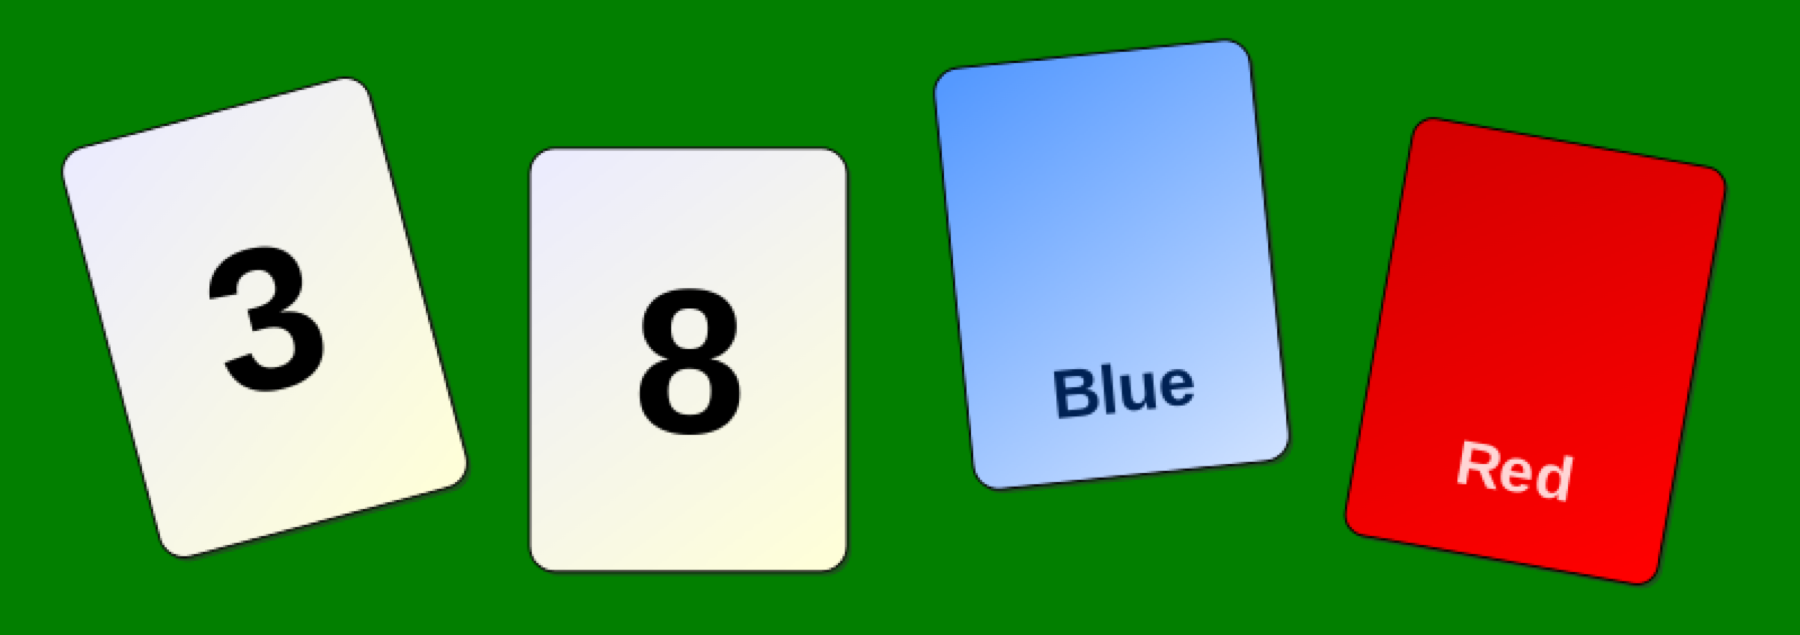
\includegraphics[width=0.5\textwidth]{figures/wason.png}
        \tiny \captionof{figure}{Image by User:Life of Riley and User:Domdomegg, CC BY-SA 4.0 via Wikimedia Commons.}

        \tiny License: \url{https://creativecommons.org/licenses/by-sa/4.0}
    \end{center}
    \indent 多くの人は\enquote{8}と\enquote{青}と答えるでしょう。確かに、\enquote{8}は確認する必要があります。裏側が青でなければ、ルールは破られていることになります。一方で、青いカードを裏返してもルールのテストにはなりません。ルールは偶数について述べているだけで、奇数については何も述べていないからです。これが、ほとんど誰も\enquote{3}のカードを確認しない理由でしょう。つまり、青いカードの裏が偶数であろうと奇数であろうと、ルールには影響しません。鍵を握るのは\enquote{赤}のカードです。これを裏返して偶数が出てきたら、ルールは破られていることになります。

    \is{counter-example}私たちの目標は、ルールを肯定するだけでなく、ルールが機能しない状況、つまり反例（counter-examples）を探すことでもあります。これは言語学的な概念の定義においても同様に重要です。メンバーでないものを含めたり、メンバーであるものを除外したりする定義は、良い定義とは言えません。\enquote{動作を表す言葉}を動詞の定義として評価する場合、肯定的な証拠と否定的な証拠の両方を考慮する必要があります。たとえば、\mention{run} という単語が\enquote{動作を表す言葉}であるか（そうです）、そして動詞であるか（そうです）を確認できます。一方で、\mention{action} や \mention{I went for a run} という文の \mention{run} のように、\enquote{動作を表す言葉}と考えられているのに動詞ではない単語などの否定的な証拠も探す必要があります。また、\mention{exist} や \mention{sense} のような必ずしも\enquote{動作を表す言葉}と認識されない単語も動詞になり得ます。\is{thinking trap!confirmation bias|)}

\end{tblsframed}

\is{noun, noun phrase (NP)!vs verb|(}\is{verb, verb phrase (VP)!vs noun|(}しかし、ここで何かを救済できるかもしれません。物理的な対象を表す言葉で、動詞であるものを思いつきますか？少し考えてみてください。

\bigskip

\is{noun, noun phrase (NP)!denotation}名詞と動詞はどちらも動作を表すことができると言って差し支えありませんが、\is{verb, verb phrase (VP)!denotation}動詞は決して物理的な対象や、人、場所を表すことはありません。そのためには名詞が必要です。このことは、私たちを次のような結論に導きます。
\ea
    \ea \enquote{人、場所、物は名詞によってのみ表される}というのは真ですが、
    \ex \enquote{名詞は人、場所、物のみを表す}というのは偽です。
    \z
\z
これは微妙な違いですが、重要な違いです。名詞はより多様なものを表すことができる一方で、動詞はより限定的であり、名詞と動詞が表すことができるものの集合は重なり合っています。\is{noun, noun phrase (NP)!vs verb|)}\is{verb, verb phrase (VP)!vs noun|)}

これまで、名詞と動詞を定義する際の3つの問題を特定しました。形容詞や他の語彙範疇に関しても同様の点が当てはまりますが、ここで一旦状況を整理しておきましょう。
\begin{enumerate}[noitemsep]
    \item 必要十分条件を用いた単純な定義は、属さないものを含めてしまい（グレービーソースはストックから作られますがスープではありません）、属するものを除外してしまいます（ガスパチョは冷たくして提供されますがスープです）。
    \item 念頭にある例に合うように定義を作るだけではいけません。意識的に\is{counter-example}反例（counter-examples）を考える必要があります。
    \item 自分の考えを正確に表現するために、言い換える必要がある場合があります。
\end{enumerate}\is{definition!linguistic!challenge|)}

語学教師として、私たちは\term{noun}（名詞）や\term{verb}（動詞）といったカテゴリー（範疇）をよく使います。しかし、単語を分類することはツールであり、最終目標ではありません。分類の目的は、世界について、あるいは今回の場合であれば言語について、一般的な記述ができるようにすることです。

これがなぜ重要なのかというと、間違ったカテゴリーは、必要以上に多くの\enquote{規則}と\enquote{例外}を生み出してしまうからです。正しいカテゴリーを持つということは、より少ない言葉でより多くのことを説明できるということであり、これによりあなたとあなたの生徒たちの両方にとって負担が軽減されます。

\bigskip

\begin{tblsframedsymbol}{質問}{test}
\begin{enumerate}[noitemsep, leftmargin=*]
    \item このコースの主な目標は何ですか？
    \item 英語の名詞は人、場所、物の名前であるという考えの何が間違っているのでしょうか？
    \item 次のうち、英語の動詞の必要十分な定義となっている文はどれですか： A) 動詞は動作を表す。 B) 動作は動詞によって表される。 C) どちらでもない。\is{necessary and sufficient conditions}
    \item スープのビデオは、単語のカテゴリーを定義することとどのように関連していますか？
    \item 私たちが避けるべき\enquote{思考の罠}とは何ですか？
\end{enumerate}
\end{tblsframedsymbol}

\begin{tblsfilled}{解答}
\begin{enumerate}[noitemsep, leftmargin=*]
    \item 言語分析の能力を高め、生徒が英語をどのように話すかを決定する際に使えるツールを提供できるようにすることです。
    \item 英語において、名詞は動作や特徴など、これよりもはるかに幅広い概念を表すからです。
    \item C) が正解です。動詞というカテゴリーは、その指示対象に基づいて確実に定義することはできません。
    \item 一般的に、カテゴリーには必要十分な特性がないことを説明しています。
    \item 自分の仮説を裏付ける肯定的な証拠だけを探し、仮説を覆すかもしれない証拠を探し損ねてしまうことです（確証バイアス）。
\end{enumerate}
\end{tblsfilled}

\subsection{\mention{phrase} とは何か}\label{sec:phrases}

\is{phrase!technical vs everyday meaning|(}名詞や動詞の場合と同じで、言語についてのごく基本的な思い込みでも、私たちを簡単につまずかせます。たとえば \mention{phrase} という語を考えてみてください。たぶん意味は分かっていると思っているでしょう。実際、日常でもよく使う語です。日常語としての \mention{phrase} は、\mention{on the table} や \mention{be going to} のように、ひとまとまりになって一つの考えを表す語の並び、といった意味でしょう。これはこれで立派な意味です。もっとも一般的な意味ですし、多くの人がこの語にまず結びつける意味でもあります。

けれども、ここで私が使うのは専門的な意味です。\is{phrase!as a headed structure|(}英語文法でいう \term{句（phrase）} とは、次の二つの性質をもつ特定の構造を指します。
\begin{enumerate}[noitemsep]
    \item その句全体の基本的な性質を決める中核語、すなわち \is{head (function)!in phrase structure}\term{主要部（head）} がある
    \item 主要部の意味を修飾したり補ったりする、任意の語や句、すなわち \is{dependent (Dep)}\term{従属部（dependent）} をもつことがある
\end{enumerate}\is{phrase!as a headed structure|)}
これは、単に \enquote{一緒に使われる語のまとまり} という日常的な理解とはかなり違います。たとえば \mention{coffee and tea} は日常感覚では十分に一つのフレーズに見えるかもしれませんが、専門的には単一の句ではありません。これは \mention{coffee} と \mention{tea} という二つの名詞句を \mention{and} で結んだ coordination であり（coordination については Section~\ref{sec:coordination} で詳しく見ます）、この表現全体を支配する単一の主要部がないからです。

日常的な意味では \enquote{phrase} と言えそうでも、専門的な意味では句ではない例として、次のようなものがあります。

\setlength{\columnsep}{0pt}
\begin{multicols}{2}
\ea
    \ea \label{ex:missing_dependents} can't help but
    \ex let alone
    \ex \label{ex:missing_dep_context} {\ob}want to{\cb} try again
    \ex {\ob}pick up{\cb} the pencil
    \ex good or bad\label{ex:missing_head}
    \ex  salt and pepper
\z
\z
\end{multicols}
(\ref{ex:missing_dependents}a, b) の例は、必要な従属部が欠けています。たとえば \mention{this isn't working, let alone} だけでは言い切れません。（\ref{ex:missing_dep_context}c, d）では、角括弧で囲った部分は、もとの文脈の中なら完全な句になりえますが、ここでは人工的に切り出されています。

一方、(\ref{ex:missing_head}e, f) の coordination の例は、また別の問題を示しています。ここで見ているような主要部をもつ構造とは違い、coordination は同格の要素を横に並べる構造で、全体を代表する一つの主要部をもちません。\mention{salt and pepper} では、一方の名詞がもう一方を支配しているわけではなく、両者が対等に並んでいます。この点で、coordination は、主要部を必要とする専門的意味での句とは根本的に異なります。

今の段階では、句とは何かを深く考え込みすぎる必要はありません。ただ、これから私が \mention{phrase} という語を、見た目にはなじみがあるけれど、実は少し違う意味で使うのだということだけ、まずは意識しておいてください。\is{phrase!technical vs everyday meaning|)}

この、\mention{phrase} の日常的な意味と専門的な意味のズレは、特に珍しいことではありません。学術の世界では、日常語を取り込んで、少し限定した専門的意味で使うことがよくあります。だからといって日常的な意味が間違いで、専門的な意味だけが正しい、というわけではありません。語には複数の意味があるのが普通です。ただし英語教師にとっては、\mention{phrase} のような言語学用語には、日常語の意味に似ていても少し違う専門的意味がある、と知っておくことが大切です。

この専門的な意味での句の定義は、これ以降の章でずっと重要になります。名詞句や動詞句やそのほかの句について話すとき、私たちが指すのは、従属部があるかどうかにかかわらず、こうした主要部をもつ構造であって、単なる語の並びではありません。はっきり言えば、そのため (\ref{ex:one-word-phrases}) の斜体のように、一語だけの句も認められます。

\ea \label{ex:one-word-phrases}
    \ea \emph{Stop}!
    \ex Would you like \emph{pepper} with that?
\z\z
\mention{phrase} の意味を少しはっきりさせたので、次は英語に見られる具体的な句の種類、まずは名詞句と、その主要部である名詞を見ていきましょう。

\section{名詞と名詞句}\label{sec:nouns}

\is{noun, noun phrase (NP)!definition challenge|(}\is{noun, noun phrase (NP)!properties of|(}完璧な \term{名詞（noun）} の定義はありません。\footnote{本書は英語についての本です。したがって、特に断らない限り、ここでいう名詞・動詞・時制などは英語のものを指します。言語一般について話すときは、その都度そう明示します。} それは \mention{soup} の完璧な定義がないのと同じです。ただし、\mention{can}、\mention{almost}、\mention{typically} といった慎重な言い方を受け入れるなら、かなり近いところまでは行けます。

ここでは、まだ説明していない語を使うことがあります。もどかしく感じるかもしれませんが、それは避けられません。統語論はシステムであり、その要素は互いとの関係の中でしか定義できないからです。意味はこの先すぐ見えてきますし、用語については Glossary にまとめてあります。

\begin{itemize}[noitemsep]
    \item 名詞は、ほとんど何でも表せます。
    \item 人・場所・物を表す語は名詞です \\（ただし \enquote{名詞とは人・場所・物を表す語である} ではありません）。
    \item 数えられる語は名詞です \\（ただし \enquote{すべての名詞が数えられる} わけではありません）。
    \item 複数形である語のほとんどは名詞です（ただし \enquote{すべての名詞が複数形になれる} わけではありません）。
    \item 名詞はしばしば \mention{the} や \mention{a} の後に現れます（ただし \enquote{\mention{the} や \mention{a} の後に来る語は名詞である} ではありません）。
    \item 名詞句（NP）の主要部は名詞です。
    \item 名詞句はふつう、修飾語として形容詞句を含むことができます \\（ほかのタイプの句では、ふつうそうなりません）。
    \item 名詞句はふつう、修飾語として副詞句を含めることができません \\（ほかのタイプの句では、ふつうできます）。
    \item \is{noun, noun phrase (NP)!functions as subject/object}名詞句は、主語や目的語をはじめ、さまざまな機能を果たせます（ただし \enquote{主語や目的語は名詞句である} という意味ではありません）。\footnote{このあと例を示しますし、主語と目的語についても後で詳しく説明します。}
    \item \is{noun, noun phrase (NP)!possessive}名詞句はふつう所有格にできます。\footnote{\textit{The Cambridge grammar of the English language} では、関係が必ずしも所有ではないため、\term{所有格（possessive）} ではなく \term{属格（genitive）} という用語を使っています。ただし \term{possessive} のほうがずっと一般的なので、本書ではこちらを使います。ただし \mention{your pet's vet} が、ペットに \enquote{所有されている} 獣医の意味ではないことだけは忘れないでください。}
\end{itemize}\is{noun, noun phrase (NP)!properties of|)}\is{noun, noun phrase (NP)!definition challenge|)}

大事なのは、こうした特徴の一つ一つが、英語学習者には奇妙に見えたり、なじみがなかったりしうることです。たとえば、学習者のほかの言語には複数形の名詞がないかもしれません。つまり、この定義の要素は、そのまま英語学習者にとって学ぶ価値のある英語の事実になっています。また、これらの記述の多くは可換ではない、という点も重要です（掛け算は可換でも割り算は可換ではありません。$X \times Y = Y \times X$ ですが、$X \div Y \neq Y \div X$ です）。要するに、言い方の違いがそのまま内容の違いになることがあるのです。

残念ながら、人はしばしば \enquote{名詞はたいてい \mention{the} や \mention{a} の後に現れる} と \enquote{\mention{the} や \mention{a} の後に現れる語はたいてい名詞である} の違いに気づきません。あるいは、いったん気づいても後で取り落としてしまいます。実際には、\mention{the} の直後に名詞が来るのは100万語あたり約34,500回ですが、名詞以外が来るのは約48,400回です。\footnote{Corpus of Contemporary American English \citep{COCA} に基づく著者の計算。} つまり、\mention{the} の次の語が名詞であることはたしかに多いのですが、それを頼りにすると、当たる回数より外す回数のほうが多くなってしまいます。

\subsection{いくつかの例}\label{sec:examples}
以下では、今挙げた特徴を例によってもう少し具体的にしていきます。それぞれの例を見たあとで、その性質の一つ以上を \enquote{もたない} 名詞を考えてみてください。言い換えれば、反例を探してみてください。\is{counter-example}


\subsubsection*{名詞が表すもの（指示対象）}
\is{noun, noun phrase (NP)!denotation}名詞が動作を表すことができることはすでに見ました。また、特徴（例：\mention{beauty}、\mention{happiness}、\mention{size}、\mention{aptitude}）、状態（例：\mention{absence}）、関係（例：\mention{togetherness}、\mention{superiority}）など、多岐にわたります。

\subsubsection*{可算性}

\is{countability (count vs non-count noun)|(}可算名詞（count nouns）の例をいくつか挙げます：\mention{apple}、\mention{book}、\mention{chair}、\mention{pen}、\mention{tree}、\mention{giraffe}、\mention{telescope}、\mention{flute}、\mention{cathedral}、\mention{quasar}、\mention{enzyme}。そして、こちらは不可算名詞（non-count nouns）の例です：\mention{water}、\mention{information}、\mention{rice}、\mention{music}、\mention{furniture}、\mention{advice}、\mention{syrup}、\mention{flour}、\mention{machinery}、\mention{courage}、\mention{syntax}、\mention{kinship}。

\subsubsection*{複数形の名詞}
\is{noun, noun phrase (NP)!plural form}次の複数形名詞の例を考えてみてください：\mention{we}、\mention{women}、\mention{children}、\mention{students}、\mention{things}、\mention{eyes}、\mention{police}、\mention{fish}、\mention{words}、\mention{thanks}、\mention{feet}、\mention{problems}。

\subsubsection*{\mention{the} または \mention{a} の後に続く名詞}
これらの例は、\mention{the} と \mention{a} に主要部名詞が加わった非常に単純な名詞句です：\mention{the world}、\mention{a lot}、\mention{the way}、\mention{the end}、\mention{the people}、\mention{a man}、\mention{the day}、\mention{a couple}、\mention{a year}。

\subsubsection*{形容詞句の修飾語と主要部名詞を持つ名詞句}
\is{modification, modifier!in NP}次に、形容詞句の修飾語と主要部名詞を持つこれらの名詞句を調べます。形容詞句は斜体で、主要部名詞はスモールキャピタルで示されています：\textit{a \emph{long} \textsc{time}}、\textit{a \emph{little} \textsc{bit}}、\textit{\emph{other} \textsc{people}}、\textit{the \emph{twelfth} \textsc{one}}、\textit{the \emph{supreme} \textsc{court}}、\textit{a \emph{very good} \textsc{morning}}、\textit{the \emph{only} \textsc{way} I know}、\textit{an \emph{old} \textsc{man}}、\textit{\emph{social} \textsc{media}}。

\subsubsection*{主語として機能する名詞句}
\is{subject (Subj)}次の各文で、斜体になっている名詞句が主語です：\textit{\emph{you} win}; \textit{\emph{time} is on my side}; \textit{\emph{a little bit} goes a long way}; \textit{\emph{other people} can help}; \textit{\emph{the supreme court} released its decision}; \textit{often, \emph{the twelfth one} is perfect}; \textit{\emph{a very good morning} is a rare pleasure}; \textit{on Monday, \emph{the shop} will be closed}; \textit{what do \emph{human rights} mean}。


\subsubsection*{所有格の名詞句}
\is{noun, noun phrase (NP)!possessive}次の名詞句は所有格です：\mention{my}、\mention{mine}、\mention{its}、\mention{whose}、\mention{Brett's}、\mention{time's}、\mention{other people's}、\mention{the supreme court's}、\mention{the lady who lives here's}。

\subsubsection*{名詞の\enquote{良い}例}
たとえば \mention{school} のような単語は、上記のすべての特性を持っています。それはプロトタイプ的な名詞であり、\enquote{良い}例です。以下は、一般的な名詞の良い例ですが、必ずしも上記のすべての特性をそれぞれ備えているわけではありません：\mention{person}、\mention{way}、\mention{day}、\mention{life}、\mention{man}、\mention{school}、\mention{student}、\mention{thing}、\mention{house}、\mention{family}、\mention{work}、\mention{part}、\mention{night}、\mention{country}、\mention{government}、\mention{place}、\mention{money}、\mention{water}、\mention{room}。どの名詞にどの特性が欠けているでしょうか？

\subsubsection*{名詞の\enquote{あまり良くない}例}
たとえば \mention{umbrage}（立腹）のような単語は、上記の特性のいくつかを欠いています。たとえば、複数形がなく、\mention{umbrage} を主要部とする所有格のNPも見つかりません。物理的な対象、人、場所を表しません。数えられないため、\mention{an} の後には続きません。他にも奇妙な点があります。何か思いつきますか？

他のあまり良くない例には、\mention{contemplation}、\mention{crockery}、\mention{furniture}、\mention{sake}（\mention{for heaven's sake} における）、\mention{shrift}、\mention{what}、\mention{behalf} が含まれます。これらにはそれぞれどのような特性が欠けているでしょうか？1つまたは複数の特性が欠けている名詞を考える練習をしてください。単語が名詞であるかどうかわからない場合は、良い辞書を使って確認してください。\footnote{私は \textit{Simple English Wiktionary}\footnote{\url{https://simple.wiktionary.org/wiki/Main_Page}} をお勧めします。私はそこの編集者であり、そこでのカテゴリーシステムを保証します。そこで探している単語が見つからない場合は、\textit{Longman Dictionary of Contemporary English}\footnote{\url{https://www.ldoceonline.com/}} を試してください。}\is{countability (count vs non-count noun)|)}


\begin{tblsframedsymbol}{質問}{test}
各グループの文から、真であり、かつ関連性のあるものを1つ選んでください。\footnote{\rotatebox{180}{\parbox[t]{0.9\linewidth}{1. a; 2. a; 3. c; 4. b; 5. a; 6. c
    }}
}
    \begin{enumerate}[noitemsep, leftmargin=*]
        \item\begin{enumerate}[noitemsep]
            \item 名詞は、物、行動、特徴などほとんど何でも表す。
            \item 名詞とは、人、場所、物のみを表す単語である。
        \end{enumerate}
        \item\begin{enumerate}[noitemsep]
            \item 数えられる単語はすべて名詞である。
            \item 名詞を数えることができる。
            \item すべての名詞は数えられる。
        \end{enumerate}
        \item\begin{enumerate}[noitemsep]
            \item 複数形の名詞は常に \mention{-s} で終わる。
            \item どんな名詞でも複数形になり得る。
            \item 複数形である単語のほとんどは名詞である。
        \end{enumerate}
        \item\begin{enumerate}[noitemsep]
            \item 名詞とは、\mention{the} または \mention{a} の後に続く任意の単語である。
            \item 名詞は典型的に \mention{the} または \mention{a} の後に続くことができる。
            \item 典型的に \mention{the} または \mention{a} の後に続く単語はすべて名詞である。
        \end{enumerate}
        \item\begin{enumerate}[noitemsep]
            \item 名詞句は典型的に、修飾語として形容詞句を含むことができる。
            \item 名詞句は典型的に、修飾語として副詞句を含むことができる。
            \item 形容詞句を修飾語として持つ句はすべて名詞句である。
        \end{enumerate}
        \item\begin{enumerate}[noitemsep]
            \item 名詞自体が、主語や目的語を含むさまざまな機能を果たすことができる。
            \item 名詞句は主語または目的語としてのみ機能する。
            \item 名詞句は、主語や目的語を含むさまざまな機能を果たすことができる。
        \end{enumerate}
    \end{enumerate}
\end{tblsframedsymbol}



\begin{tblsframedsymbol}{名詞を見つけましょう}{pencil}
    In reality, from the top of the ladder, standing erect on the last rung, you could just touch the Moon if you held your arms up. We had taken the measurements carefully (we didn't yet suspect that she was moving away from us); the only thing you had to be very careful about was where you put your hands. I always chose a scale that seemed fast (we climbed up in groups of five or six at a time), then I would cling first with one hand, then with both, and immediately I would feel ladder and boat drifting away from below me, and the motion of the Moon would tear me from the Earth's attraction. Yes, the Moon was so strong that she pulled you up; you realized this the moment you passed from one to the other: you had to swing up abruptly, with a kind of somersault, grabbing the scales, throwing your legs over your head, until your feet were on the Moon's surface.\footnote{\rotatebox{180}{\parbox[t]{0.9\linewidth}{
        \mention{reality}, \mention{top}, \mention{ladder}, \mention{rung}, \mention{you}, \mention{Moon}, \mention{you}, \mention{your}, \mention{arms}. \mention{We}, \mention{measurements}, \mention{we}, \mention{she}, \mention{us}; \mention{thing}, \mention{you}, \mention{you}, \mention{your}, \mention{hands}. \mention{I}, \mention{scale}, \mention{we}, \mention{groups}, \mention{time}, \mention{I}, \mention{ladder}, \mention{boat}, \mention{me}, \mention{motion}, \mention{Moon}, \mention{me}, \mention{Earth's}, \mention{attraction}. \mention{Moon}, \mention{she}, \mention{you}; \mention{you}, \mention{moment}, \mention{you}, \mention{other}; \mention{you}, \mention{kind}, \mention{somersault}, \mention{scales}, \mention{your}, \mention{legs}, \mention{your}, \mention{head}, \mention{your}, \mention{feet}, \mention{Moon's}, \mention{surface}.
    }}}\\\phantom{~}\hfill~-- イタロ・\citeauthor{calvino2018}、\enquote{月の距離}

\end{tblsframedsymbol}

\subsection{可算性}\label{sec:count}

\is{countability (count vs non-count noun)|(}\is{number|(}可算性という考え方自体はとても単純です。名詞を $x$ として \enquote{two $x$} と言えるなら、$x$ は可算名詞です。たとえば \mention{two pencils} は問題ないので、\mention{pencil} は可算名詞です。しかし *\mention{There are two furnitures} とは言えません（* は非文法的であることを示します）。したがって \mention{furniture} は不可算名詞です。\mention{jeans} のような語は一見すると可算名詞のように見えるかもしれませんが、実際に数えているのはジーンズそのものではなく \emph{pair} です。もう一つ意外な不可算名詞として \mention{police} があります。* \mention{two police were standing on the corner} とは言わず、\mention{two} (\mention{police}) \mention{officers} と言います。このとき可算なのは \mention{officer} です。\mention{meat} もふつうは不可算ですが、\enquote{肉の種類} という意味なら可算になります。このように、\enquote{種類} の意味で不可算名詞を可算名詞として使うのは、かなり普通のことです。

可算性そのものは分かりやすくても、難しいのは、どの名詞なら \enquote{two $x$} と言えて、どの名詞では言えないのかを見抜くことです。何が数えられて何が数えられないかは、あまりにも自明に思えるかもしれません。そのため、生徒に説明するのも簡単だと感じてしまうかもしれません。ひょっとすると、これが分からない学習者は要領が悪いだけでは、と心のどこかで思ってしまうかもしれません。でも、そう感じるのは、あなたがすでに知っているからです。実際には、専門家でさえ可算性をかなり取り違えることがあります。たとえば \textit{Longman Dictionary of Contemporary English} を見てみましょう。

\is{thinking trap}私はこの優れた辞書をよく引きます。項目がとても有益だからです。ところが \mention{uncountable}\footnote{\url{https://www.ldoceonline.com/dictionary/uncountable/}} を見ると、次のような定義に出会います。

\begin{quote}
    An uncountable noun has no plural form and refers to something which can't be counted or regarded as either singular or plural, for example `money' or `happiness'.\\
    （不可算名詞には複数形がなく、数えることができないもの、または単数としても複数としても見なすことができないものを指す。例：\enquote{money}や\enquote{happiness}。）
\end{quote}
残念ながら、Longman も、さきほど見たのと同じ思考の落とし穴にはまっています。定義に合う例はいくつか挙げたのに、反例を見ていないのです。では、こちらで反例を探してみましょう。複数形をもちながら、数えることはできない名詞、つまり \enquote{two $x$} と言えない複数形名詞を思いつけるでしょうか。Section~\ref{sec:examples} ですでに少なくとも一つ見ています。\is{counter-example} 少し考えてから脚注を見てください。\footnote{\rotatebox{180}{\parbox[t]{0.9\linewidth}{
        \is{plural!plural-only noun}すでに \mention{police} を見ました。\mention{Pants} も別の例です。*\mention{two pants} ではなく \mention{two pairs of pants} と言います。他にも \mention{groceries}、\mention{remains}、\mention{clothes}、\mention{scissors}、\mention{genitals} などがあります。
    }}
} おかしいのは、この辞書が個々の語にはそれなりに正しくラベルを付けていることです。たとえば \mention{glasses}\footnote{\url{https://www.ldoceonline.com/dictionary/glasses/}} の項目には、ちゃんと \term{不可算（uncountable）} と書かれています。編集者たちは \mention{glasses} が複数形で、しかも不可算名詞であることを知っているわけです。にもかかわらず、自分たちの定義と自分たちの実際の運用が食い違っていることに気づいていません。


\begin{tblsframed}{なぜ大事なのか}
    次の例を考えてみましょう。

    \ea
        \ea[]{I had (a) tea.}\label{ex:tea}
        \ex[]{I had a cookie.}\label{ex:cookiea}
        \ex[*]{I had cookie.}\label{ex:cookie}
        \z\label{ex:blank}
    \z
    \is{countability (count vs non-count noun)!and determiner}\is{determiner (Det)!and countability}(\ref{ex:tea}) は \mention{a} があってもなくても問題ありませんが、(\ref{ex:cookiea}) では \mention{a} が必要で、(\ref{ex:cookie}) は非文法的です。この違いは何で説明できるでしょうか。答えは、単数の可算名詞には \term{限定詞（determiner）} が必要だということです（この用語は後の章で詳しく説明します）。\mention{a} と \mention{the} は限定詞として働きますし、\mention{one}、\mention{his}、\mention{Brett's}、\mention{every} なども同じです。つまり、可算か不可算か、単数か複数かという見方をもっていれば、なぜ (\ref{ex:tea}) は両方とも許され、(\ref{ex:cookie}) は許されないのかを説明できます。これが、私が \enquote{私たちはシステムを相手にしている} と言うときの意味です。システムの一部が分かると、それを使って、いかにも別の話に見える領域の謎も解けるようになります。
\end{tblsframed}

このように、Longman 辞書の \mention{uncountable} の定義は、その辞書自体が全体としてはとてもよい辞書であり、しかも \mention{glasses} をはじめ多くの個別項目がその定義と食い違っているにもかかわらず、やはり間違っています。どうやら、この判断は思っていたほど簡単ではありません。とはいえ、たとえ定義づくりが少し難しいと分かったとしても、何が数えられて何が数えられないかは、何らかの性質を見れば自明に決まるはずだ、と感じるかもしれません。もし本当にそうなら、単数名詞はつねに単数、複数名詞はつねに複数として訳されるはずです（少なくとも、その言語に複数形があるならば）。\is{countability (count vs non-count noun)!cross-linguistic variation|(} ところが、可算性の領域では、ある言語で数えられるものが、別の言語では数えられないことがあるのです。

もしあなたが多言語話者であれば\is{cross-linguistic influence|(}、すでにおそらくこれに遭遇したことがあるでしょう。次のフランス語を考えてみてください：

\ea[]{\gll J' ai coupé mes cheveux.\\
     私 持つ 切る 私の-\textsc{pl} 髪-\textsc{pl}.\\
    \glt `私は髪を切った。'}\label{ex:cheveaux}
\z
\is{number!cross-linguistic variation}\refp{ex:cheveaux} において、フランス語\il{French}の単語 \mention{cheveux} は複数形の可算名詞です（フランス語でも髪の毛を数えることは稀ですが）、一方英語では通常、単数の不可算名詞です。フランス語が示しているように、髪の毛を数え上げる必要はありません。単に \mention{I cut my hairs} と言ってそのままにしておくこともできます。英語は髪を塊として扱い、フランス語は髪を個別のアイテムとして扱います。どちらがより論理的ということはありません。\is{cross-linguistic influence|)}\is{countability (count vs non-count noun)!cross-linguistic variation|)}

何が数えられるかなど、ふだん当然だと思っていることを、客観的事実だと考えるのは簡単です。けれども、この種の区別の多くは、実際には客観的事実というより、ある言語や方言の話者共同体の中で共有されている判断です。外部の人には、しばしばまったく予測できません。ややこしいのは、\mention{countable}（数えられる）という語が二つの役割を同時に担っていることです。一つは名詞の文法的な性質（数詞を取る、複数形になる）を表す役割、もう一つはその名詞が指すものの概念的な性質（個別のものとして捉えるか、まとまりとして捉えるか）を表す役割です。たいていはこの二つが重なりますが、\mention{furniture} や \mention{news} のようにずれると混乱が起こります。この種の \enquote{二重の役割} には、この先も何度か出会うはずです。

それにもかかわらず、多くの語学教材は、可算性が単なる内省から明らかであるかのように扱っています。全くそんなことはありません！子供向けの教科書である \citet{allen2008} からの以下の説明を考えてみてください。英語を話すなら全く単純ですが、そうでないならほとんど全く役に立ちません。

\begin{quote}
    You can see from the list that some nouns can be counted and others can not. For example, if you want to tell your friend about the fruit on the tree, you could tell them your tree has plenty of plums on it. The noun `plum' is countable so you have to make it plural by adding an `-s-' (sic). Or you could tell them your tree has plenty of fruit on it. In this case, the noun `fruit' is uncountable, so you can not count an `-s'. \citet[1]{allen2008}\\
    （リストから、数えられる名詞とそうでない名詞があることがわかりますね。たとえば、木に生えている果物について友達に話したい場合、あなたの木にはたくさんの\enquote{plums}が生えていると言うことができます。名詞\enquote{plum}は数えられるので、\enquote{-s-}（原文ママ）を加えて複数形にしなければなりません。あるいは、あなたの木にはたくさんの\enquote{fruit}が生えていると言うこともできます。この場合、名詞\enquote{fruit}は数えられないので、\enquote{-s}を数えることはできません。）
\end{quote}

この本は、プラムが数えられるから可算であり、可算だから数えられると仮定しています。これ以上簡単なことがあるでしょうか？では \mention{rice} や \mention{seed} はどうでしょうか？\enquote{2粒の米}を意味する場合に \mention{two seeds} とは言えるのに *\mention{two rices} とは言えないことを、英語学習者が推測する方法はありません。\mention{Two rices} は\enquote{2種類の米}を意味するだけで、\enquote{2粒}を意味することはできません。\is{countability (count vs non-count noun)|)}\is{number|)}

\begin{tblsframedsymbol}{練習問題}{pencil}
    各項目について、名詞が単数か複数か、そしてそれが名詞の数えられる意味か数えられない意味かを判断してください。\\
    例：\mention{The two fish escaped.} （可算、複数）

    \begin{enumerate}[noitemsep, leftmargin=*]
        \item \mention{The data were accurate.}
        \item \mention{The data was accurate.}
        \item \mention{The Canadian media are generally reliable.}
        \item \mention{The Canadian media is generally reliable.}
        \item \mention{The sheep are grazing.}
        \item \mention{Little difference could be seen.}
        \item \mention{A run will be calming.}
        \item \mention{a little sugar}
        \item \mention{made of rock}
        \item \mention{The remains are buried here.}
        \item \mention{More suction, please.}
        \item \mention{Pizza is tasty.}
        \item \mention{Eating lamb is less common here.}
        \item \mention{two or three times}
        \item \mention{The children are studying.}
        \item \mention{A little knowledge can be dangerous.}
        \item \mention{the police}
        \item \mention{some new jeans}
        \item \mention{two coffees}
        \item \mention{new employment statistics}
        \item \mention{a little time}
    \end{enumerate}
\end{tblsframedsymbol}

\section{動詞と動詞句}\label{sec:verbs}

\is{verb, verb phrase (VP)|(}では、英語の動詞については何が言えるでしょうか。まずは、いかにも動詞らしい典型例を並べてみます。
\ea
    \emph{jump}, \emph{walk}, \emph{ask}, \emph{turn}, \emph{work}, \emph{move}, \emph{play}, \emph{pull}, \emph{reach}, \emph{laugh} \label{ex:verblist}
\z
\is{verb, verb phrase (VP)!vs noun|(}\is{noun, noun phrase (NP)!vs verb|(}これらは動作を表す語でしょうか。たしかにそうです。けれども、これが名詞のリストにもなりうることに気づいたでしょうか。
\ea\label{ex:verb-list-as-nouns}
    \ea She missed the \emph{jump}.
    \ex I went for a \emph{walk}.
    \ex That's a pretty big \emph{ask}.
    \ex Give it a \emph{turn} and see.
    \ex I went to \emph{work}.
\z
\z
上の斜体語は、それぞれ名詞です。（疑わしいなら、さきほど見た性質に照らしてみてください。）ところが、次の文では同じ綴りの語が動詞になっています。

\ea\label{ex:verb-list-as-verbs}
    \ea She \emph{jumped} the gap.
    \ex I \emph{walk} the dog each morning.
    \ex He's \emph{asking} for a \$10,000 raise.
    \ex It's hard to \emph{turn} the knob.
    \ex I \emph{work} in Toronto.
\z
\z
では、名詞と動詞の違いはどう見分ければよいのでしょうか。文脈に置かれるまで分からないこともあります。形のうえでは同じでも、機能はまったく違います。\refp{ex:verblist} のリストは完全に曖昧です。\is{verb, verb phrase (VP)!vs noun|)}\is{noun, noun phrase (NP)!vs verb|)} それでも、動詞には一般に次のような性質があります（例はこのあと示します）。

\begin{itemize}[noitemsep]
    \item \is{verb, verb phrase (VP)!denotation}動詞は典型的に動作や状態を表し、物理的な対象は表しません。
    \item \is{verb, verb phrase (VP)!forms (-\textit{s}, -\textit{ing}, past)|(}過去形をもつ語は動詞です（ただし、すべての動詞に過去形があるわけではありません）。
    \item ほぼすべての動詞には \mention{-s} 形があります（例外もあります）。
    \item ほぼすべての動詞には \mention{-ing} 形があります（例外もあります）。
    \item ほぼすべての動詞は不定詞マーカー \mention{to} の後に来ることができます。\is{verb, verb phrase (VP)!forms (-\textit{s}, -\textit{ing}, past)|)}
    \item 動詞は形容詞句では修飾されません。
    \item \is{verb, verb phrase (VP)!modified by adverb phrase}動詞はふつう副詞句で修飾できます。
    \item 動詞句の主要部は必ず動詞です。
    \item \is{verb, verb phrase (VP)!head}\is{clause!headed by verb phrase}節の主要部は必ず動詞句です。
    \item \is{agreement!subject--verb}動詞はしばしば、その節で主語として機能する句と一致関係を結びます。
\end{itemize}

いくつか例を見てみましょう。

\subsubsection*{動詞が表すもの}
\is{verb, verb phrase (VP)!denotation}これらは専門的な分類ではなく、あくまで日常的な分類であり、他のタイプをリストに追加することもできます。

\ea Verbs（動詞）:\\
    actions（動作）: come, go, wave, run, swim, play, hit\\
    mental activities（精神活動）: consider, wonder, decide, recall\\
    states（状態）: be, seem, own, need, taste, matter, appear, exist\\
    mental states（精神状態）: believe, know, agree, mind, like\\
    accomplishments（達成）: win, sleep, become, remain, relax, stop, fail
\z

\subsubsection*{過去形}\label{sec:past-forms}
\is{verb, verb phrase (VP)!forms (-\textit{s}, -\textit{ing}, past)}動詞はほぼ常に過去形を持ちますが、名詞は決して持ちません。（過去形を持たない動詞を思いつきますか？\footnote{\rotatebox{180}{\parbox[t]{0.9\linewidth}{
        \is{defective verb}私の知る限り、\mention{Must}、\mention{beware}、\mention{ought} だけが過去形を持たない動詞です。1つ以上の形が欠けている動詞は\term{defective}（不完全）であると言われます。
    }}})\\

\ea\label{ex:past-tense-forms-verbs-vs-nouns}
    \ea Verbs（動詞）:\\
    \begin{tabular}{@{} l l l l l l l}
    want & $\rightarrow$ & wanted && play & $\rightarrow$ & played \\
    go & $\rightarrow$ & went && come & $\rightarrow$ & came \\
    run & $\rightarrow$ & ran && make & $\rightarrow$ & made \\
    is & $\rightarrow$ & was && are & $\rightarrow$ & were \\
    \end{tabular}
    \ex Nouns（名詞）:\\
    \begin{tabular}{@{} l l l l l l l}
    magazine & $\rightarrow$ & n/a && jeans & $\rightarrow$ & n/a \\
    idea & $\rightarrow$ & n/a && government & $\rightarrow$ & n/a \\
    \end{tabular}
\z
\z
\is{word family}\refp{ex:verblist} にあるような、歴史、綴り、発音を共有する名詞と動詞がたくさんあります。それらは同じ\hyperref[sec:family-lemma-shape-token]{語族（word family）}に属していますが、私と兄弟が同じレイノルズ家に属していながらも別々の人間であるのと同じように、別の単語です。



\subsubsection*{その他の動詞の形}
\is{verb, verb phrase (VP)!forms (-\textit{s}, -\textit{ing}, past)}ほとんどすべての動詞は、原形に加えて \mention{-s} 形と \mention{-ing} 形も持っています。

\ea
run $\rightarrow$ runs $\rightarrow$ running\\
go $\rightarrow$ goes $\rightarrow$ going\\
try $\rightarrow$ tries $\rightarrow$ trying\\
make $\rightarrow$ makes $\rightarrow$ making\\
do $\rightarrow$ does $\rightarrow$ doing\\
have $\rightarrow$ has $\rightarrow$ having\\
contemplate $\rightarrow$ contemplates $\rightarrow$ contemplating\\
recondition $\rightarrow$ reconditions $\rightarrow$ reconditioning
\z

これらの形を欠いている動詞を思いつきますか？\footnote{\rotatebox{180}{\parbox[t]{0.9\linewidth}{
        \is{defective verb}\mention{Can}、\mention{may}、\mention{will}、\mention{shall}、\mention{must}、\mention{ought} は、これらの形を欠いている最も一般的な動詞です。
    }}
}

\subsubsection*{動詞句における修飾語}
\is{modification, modifier!in VP}\is{adjective, adjective phrase (AdjP)!as modifier in NP}動詞句は典型的に副詞句を修飾語として許容しますが、形容詞句は許容しません。以下は副詞句によって修飾された動詞句の例です： \mention{run quickly}、\mention{think deeply}、\mention{try consistently}、\mention{always be good}、\mention{easily do it}、\mention{happily help}。比較のために、形容詞句によって修飾された対応する名詞句を挙げます： \mention{a quick run}、\mention{deep thoughts}、\mention{consistent effort}、\mention{an easy goal}、\mention{the happy helper}。

\subsubsection*{動詞は動詞句の主要部になる}
\is{head (function)}それぞれの例は動詞句です。括弧は、大きな動詞句の中にある小さな動詞句を囲んでいます：\textit{\emph{try}}、\textit{never \emph{go} to school}、\textit{\emph{had} a new idea}、\textit{usually \emph{playing} tennis with a friend}、\textit{\emph{have} }(\textit{\emph{finished} dinner})、\textit{\emph{may} }(\textit{\emph{be} }(\emph{leaving} soon))

\subsubsection*{節の主要部としての動詞句}
\label{sec:VPs_head_clauses}
\is{verb, verb phrase (VP)!head}\is{clause!headed by verb phrase}それぞれの例は節です。動詞句は斜体になっています。\textit{Dogs \emph{never go to school}.}  \textit{She is \emph{usually playing tennis with a friend}.} \textit{Who \emph{had a new idea}?} \textit{The folks at table 5 \emph{have finished dinner}.} \textit{I \emph{may be leaving soon}.} \textit{\emph{Try.}}

\subsubsection*{主語との一致}\label{sec:agreement}
\is{agreement!subject--verb|(}\is{agreement!and third person singular|(}\is{subject (Subj)!agreement with verb|(}現在形の動詞の場合、主語が三人称単数であれば、動詞は典型的に \mention{-s} 形で現れることで主語と\enquote{一致（agree）}します。三人称の名詞句とは、一人称（\mention{I}、\mention{me}、\mention{myself}、\mention{we}、\mention{ours} など）でも二人称（\mention{you}、\mention{yours}、\mention{yourself}）でもないもののことです。

\ea
    \ea She studies English.\\（\emph{She} は三人称単数であり、現在形動詞 \emph{studies} の末尾の \emph{-s} が呼応を示しています。）
    \ex She studied English.\\（\emph{She} は三人称単数ですが、動詞は過去形です。）
    \ex They study English.\\（\emph{They} は単数ではありません。）
    \z
\z\is{subject (Subj)!agreement with verb|)}\is{agreement!and third person singular|)}\is{agreement!subject--verb|)}\is{verb, verb phrase (VP)|)}

\subsection{助動詞}\label{sec:aux}

\is{auxiliary verb|(}\is{auxiliary verb!NICER properties|(}表~\ref{tab:NICER} に示すように、\term{auxiliary verbs}（助動詞）と呼ばれる動詞の小さな下位範疇があります。これらは\term{NICER}特性 \citep{sag2019} を持っています。

\begin{table}
    \begin{tabularx}{0.80\textwidth}{@{} >{\centering\arraybackslash\hsize=.03\hsize}X >{\hsize=.21\hsize}X >{\hsize=.38\hsize}X >{\hsize=.38\hsize}X @{}}
    \lsptoprule
    \multicolumn{2}{>{\hsize=.24\hsize}X}{Feature（特徴）} & Examples（例） & Counter-examples（反例） \\
    \midrule
    N & egation（否定）:& Lee \emph{will} not eat. & *Lee eats not. \\
    I & nversion（倒置）:& Lee \emph{has} eaten. \(\rightarrow\) \newline \emph{Has} Lee eaten? & *Eats Lee? \\
    C & ontraction（短縮）:& didn't, shouldn't & *eatn't, *keptn't \\
    E & llipsis（省略）:& Kim \emph{was} eating, and \newline Lee \emph{was} ..., too. & *Kim kept eating, and \newline Lee kept ..., too. \\
    R & ebuttal（反論）:& I did tóo/só read it. \newline Did not! & *I tried tóo/só to read it. *Tried not! \\
    \lspbottomrule
\end{tabularx}
\caption{NICER特性}\label{tab:NICER}
\end{table}\is{auxiliary verb!NICER properties|)}
\noindent これらには\is{modal auxiliary verb}\term{法助動詞（modal auxiliary verbs）}が含まれます：
\ea\label{ex:modal-auxiliaries-list}
    \ea will/won't; would/wouldn't
    \ex shall/shan't; should/shouldn't
    \ex may; might/mightn't
    \ex can/can't; could/couldn't
    \ex must/mustn't
\z
\z
\noindent そして他にもいくつかあります：
\begin{itemize}[noitemsep]
    \item \mention{be}、\mention{do}（\hyperref[ch:questions]{疑問文}用）、および \mention{have}（完了形用）
    \item \mention{need}、\mention{dare}、および \mention{ought}（法助動詞として。ただし北米では典型的ではない）
\end{itemize}


ここでも、まだ定義していない用語を使って説明しています。もどかしく感じるかもしれませんが、これは避けられないことです。統語論はシステムであり、その要素は互いの関係においてのみ定義できるからです。他の言葉の意味はすぐに明らかになります。それらに出会ったら、戻ってきてこの資料をもう一度見てみてください。

言語学習者は常にこの種のもどかしさに直面しています。それが人格を形成すると言うのは役に立ちませんが、この種の一時的な曖昧さを受け入れることができる人の方が、最終的にはより成功する傾向があるというのは事実です。\is{auxiliary verb|)}

\section{まとめ}
この章では、いくつかの重要な文法用語や概念を紹介するとともに、英語教師にとって非常に有用だと私が信じている、いくつかの思考習慣や心構えを提案しようと試みました。英語について考えるためのこれらのアプローチには、以下のものが含まれます：
\begin{enumerate}[noitemsep]
    \item 反例を探すこと：この習慣は、単純化されすぎた規則や説明を乗り越える後押しとなり、\enquote{常識}であると同時に間違っていることを生徒に教えるのを避けるのに役立ちます。
    \item 定義を精査すること：私たちが文法概念をどのように定義しているかを調べることで、学習者によりよく説明し、彼らの質問を予測することができます。
    \item 言語記述における非可換性を認識すること：\enquote{AはBを暗示する}が\enquote{BはAを暗示する}を意味しないことを理解することは、説明によくある落とし穴を避けるのに役立ちます。
    \item 自分の言語的直感に挑戦すること：熟練した英語話者として私たちに明白に見えることでも、学習者には不透明かもしれません。この認識は、生徒の苦労に共感するのに役立ちます。
    \item 用語の専門的な意味と日常的な意味を区別すること：このような区別は、おなじみの意味が私たちの理解を混乱させるのを防ぐのに役立ちます。
\end{enumerate}

重要な包括的概念は、言語がシステムであるということです。各部分は互いに依存しており、孤立して完全に理解できるものは何もありません。私たちがアイデアを織り交ぜれば織り交ぜるほど、教師である私たち自身と生徒の両方にとって、タペストリーの全体像がより鮮明に浮かび上がってくるでしょう。



\begin{tblslineshorizontal}{記述式小テスト}

指示：次の各質問に2～3文で答えてください。

\begin{enumerate}[noitemsep]
    \item 動詞を単に\enquote{動作を表す言葉}と定義できないのはなぜですか？例を用いて答えを支持してください。
    \item （たとえば \mention{walk} が）どのようにして名詞にも動詞にもなり得るのかを説明してください。そのカテゴリーを決定するものは何ですか？
    \item ほとんどの語彙動詞が取ることができる形は何ですか？例外にはどのようなものがありますか？
    \item 形容詞句と副詞句が動詞に関連して修飾語としてどのように機能するかの違いを説明してください。
    \item 動詞の\enquote{主語との一致}とはどういう意味ですか？それはいつ起こりますか？
    \item 助動詞と他の動詞を区別するものは何ですか？特性の例を2つ挙げてください。
    \item 名詞と動詞は、表すことができるものの点でどのように異なりますか？なぜこの区別が重要なのですか？
    \item 動詞、動詞句、および節の関係は何ですか？
    \item \enquote{不完全（defective）}な動詞とは何ですか？この章の例ではどの形が欠けていますか？
\end{enumerate}

\end{tblslineshorizontal}

\begin{tblsfilled}{解答}

\begin{enumerate}[noitemsep, leftmargin=*]
    \item 多くの名詞が動作を表す（例：\mention{action}、\mention{run}、\mention{walk}）一方で、一部の動詞は動作を表しません（例：\mention{exist}、\mention{seem}）。意味と文法カテゴリーの関係は、単純な動作/非動作よりも複雑だからです。

    \item \mention{walk} (名詞) と \mention{walk} (動詞) のような単語は、同じ語族に属していますが別の単語です。動詞は動詞の屈折変化をとり、動詞句の主要部となります。名詞は限定詞をとり、数によって屈折変化します。

    \item ほとんどの語彙動詞は、原形、\mention{-s} 形、および \mention{-ing} 形を持っています。実際には他にもいくつかの形がありますが、それらについては後で説明します。

    \item 副詞句は一般的に動詞句（VP）の修飾語として機能します（\mention{run quickly}）が、形容詞句は機能しません。名詞句（NP）では状況が逆転し、（\mention{a quick run}）となりますが、*\mention{a quickly run} とはなりません。

    \item 一致は、現在形の動詞の原形と三人称単数形の間で選択を行います。また、過去形においては \mention{were} と \mention{was} の間で選択を行います。

    \item 助動詞はNICER特性を持っています。これには、直接否定形を作る能力（\mention{will not}）や、主語と助動詞の倒置（\mention{Has Lee eaten?}）に参加する能力が含まれます。通常の動詞にはこれらの特性がありません。

    \item 動詞は主に動作と状態を表すことに制限されていますが、時制を通じて時間も表します。名詞はこのように制限されていません。

    \item 動詞は動詞句の主要部となり、動詞句は節の主要部となります。この階層関係は英語の文構造の基本です。

    \item 不完全な動詞とは、典型的な動詞の形の1つ以上を欠いているもののことです。この章では、過去形を欠いている \mention{must}、\mention{beware}、\mention{ought} や、\mention{-s} 形と \mention{-ing} 形を欠いている \mention{can}、\mention{may}、\mention{will}、\mention{shall}、\mention{must} のような法助動詞の例を挙げています。
\end{enumerate}

\end{tblsfilled}

\begin{tblslineshorizontal}{ディスカッション問題}

\begin{enumerate}[noitemsep]
    \item 英語における名詞と動詞の識別において、形式的特性（屈折、修飾パターン）と意味がどのように相互作用するかを議論してください。この理解は、\enquote{動作を表す言葉}や\enquote{人、場所、または物}といった過度に単純化された定義を避けるのにどのように役立ちますか？テキストから具体的な例を挙げてください。

    \item 可算性や複数形といった一見単純な概念が、言語カテゴリーの複雑でしばしば恣意的な性質をどのように明らかにしているかを説明してください。これらのカテゴリーが客観的な事実ではなく、主観間の判断である理由を説明するために、異なる言語の例を使用してください。

    \item 英語における動詞と助動詞の関係を分析してください。NICER特性は助動詞をどのように区別しますか？また、これは英語教育にどのような影響を与えますか？

    \item 語彙範疇と句範疇（たとえば、名詞と名詞句の間、または動詞、動詞句、節の間）の階層関係を考察してください。これらの専門的な関係を理解することは、教師が文法構造をよりよく分析し説明するのにどのように役立ちますか？
\end{enumerate}

\end{tblslineshorizontal}

\chapter{標準、標準英語、そして何を教えるべきか}\label{sec:standards}\label{ch:standards}

\begin{tblsframedsymbol}{学習目標}{bulb}
  \begin{itemize}[noitemsep, leftmargin=*]
      \item 品質としての \mention{standard} と慣習としての \mention{standard} の違いを区別する
      \item 標準英語（Standard English）を単一の強固なものではなく、関連する変種（varieties）の集まりとして認識する
      \item 標準英語が他の直言（dialects）よりも本質的に優れているわけではないことを理解する
      \item 文法性（grammaticality）と有意味性（meaningfulness）の違いを分析する
      \item 文法性に関する直感がなぜ当てにならないことがあるのかを理解する
      \item 処理の限界が文法性の判断にどのように影響するかを認識する
      \item 形式と意味のペアリング（form--meaning pairing）の分析を適用して、文法的な容認可能性（acceptability）を理解する
      \item 文法規範（grammatical norms）を定義する上での言語共同体（speech communities）の役割を理解する
      \item 文法に対する記述的（descriptive）アプローチと規範的（prescriptive）アプローチを区別する
  \end{itemize}
  \end{tblsframedsymbol}

\section{はじめに}
\hyperref[ch:categories]{次の章}では、語彙範疇の説明に戻りますが、ここでは、英語に関して何が正しく何が間違っているかという認識に関連するいくつかの問題について少し考える時間を割くべきでしょう。この章は、\term{標準（standards）}\is{standard|(}、\term{標準英語（Standard English(es)）}\is{Standard English|(}、\term{文法性（grammaticality）}\is{grammaticality|(}、そして\term{規範性（normativity）}\is{normativity|(}の概念について考えるのに役立つはずです。これらはすべて、英語教師が理解しておくべき重要な概念です。

なぜこれらの概念が重要なのでしょうか？教師として、私たちは英語において何が\enquote{正しい}かという裁定者になることをよく求められます。しかし、これから見ていくように、それは常に見た目ほど単純なことではありません。何が標準でしょうか？何が文法的でしょうか？そしておそらく最も重要なこととして、私たちは実際に何を教えるべきでしょうか？

まず、\enquote{標準}という概念を解きほぐし、それが言語にどのように適用されるかを見ていきます。次に、標準英語、より正確には複数の標準英語の概念と、なぜこの区別が重要なのかを探ります。さらに、文法性\is{grammaticality!questioning of|(}について深く掘り下げ、何が文法的\is{grammatical!vs meaningful|(}または非文法的\is{ungrammaticality}であるか、そしてこれに関する私たちの直感\is{intuition!about grammaticality|(}がなぜ時として誤解を招くことがあるのかを検証します。最後に、言語の規範的な側面と、それが教師としての私たちの決定にどのような影響を与えるかを考察します。

この章が終わる頃には、これらの概念についてよりニュアンスに富んだ理解を得て、英語教育という複雑な風景をナビゲートする準備がより整っているはずです。それでは、私たちが何かが\enquote{標準}であると言うときに何を意味するのかを考えることから始めましょう。

ほとんどの人にとって、\mention{standard} は肯定的な含意\is{standard!positive connotations of}を持っています。\mention{standard} と一緒に使う言葉、たとえば \mention{gold standard} と \mention{quality standard}、あるいは \mention{standard of living} と \mention{standard of care} といったペアを考えてみてください。高い基準を持っていたり、それを超えたりするのは良いことです。私たちは教育の基準、環境の基準、技術の基準\is{technology standard}\is{technology standard|(}を設定しますが、これらはすべて私たちの教育、環境、技術をより良くするためのものです。

要するに、標準とは私たちが目指すものであり、\term{標準英語（Standard English）}（大文字の \mention{S} に注目してください）は目指すべきもののように聞こえるかもしれません。それは\enquote{良い}英語、文法的な\is{grammatical!vs Standard English|(}英語、あるいは文学的な英語と同等だと思うかもしれません。しかし、定義したり目標にしたりするのは、それほど単純でも明確でも簡単なことではありません。

あなたはおそらくVHSが何であるかを知っている年齢でしょう。しかし、ベータマックス（Betamax）が何であるかを知るには若すぎるかもしれません。一時期、これらは競合するビデオテープの規格でした。ほとんどの基準で、ベータマックスの方が高品質な製品でした。画質も音質も優れていました。しかし、それは随分前に消滅したため、あなたは聞いたことすらないかもしれません。そしてVHSがビデオカセットテープとプレーヤーの標準となりました（少なくとも人々がまだVCRを使っていた間は）。

標準は良いという意味ではありませんし、良いからといって標準というわけでもありません。

さまざまな軌間（レールの幅）が存在しますが（図~\ref{fig:rail}）、標準軌\is{standard!rail gauge analogy}は幅1.435メートルです。私が住んでいるミシサガ（Mississauga）の新しいライトレール路線にはこれが使われています。しかし、東隣の都市であるトロントのトロント交通局（TTC）で伝統的に使われているトロント軌間は、幅1.495メートルです。確かにそれぞれのサイズには長所と短所がありますが、標準軌の最大の利点は、それが標準であるということです。最も一般的に使用されているため、新しい鉄道車両や中古の鉄道車両を必要とする場合、標準軌を使用する方がはるかに安く、早く手に入ります。これが、トロントのシステムと直接車両を互換させることができなくなるにもかかわらず、ミシサガがそれを選んだ理由です。この選択は品質や優位性に関するものではなく、コストと可用性に関するものでした。

標準英語\is{Standard English!not inherently superior|(}は英語の\enquote{最高}の形態ではありません。標準英語が他の方言\is{dialect!and Standard English|(}よりも本質的に優れているわけではありません。標準英語は単に、最も広く受け入れられ、最も制度化され、多様なコミュニケーション\is{communication!as function of language}のための最も一般的な共通基盤であるに過ぎません。

言語学において、\mention{standard} という言葉は、質的な指標というよりも、むしろ社会政治的な指標\is{Standard English!as a sociopolitical marker}として機能することがよくあります。それは、歴史的、文化的、そしてしばしば植民地主義的な力によって、ある方言（通常は社会的または経済的に支配的なグループの方言）が他の方言よりも引き上げられた結果なのです。

ですから、私たちが標準英語について語るとき、本当に議論しているのは、体系化され、学校で教えられ、公文書で使用され、正式な場で期待される一連の慣習のことなのです。それは知性、道徳性、あるいは価値の尺度ではありません。単に最も一般的かつ広範に期待され、受け入れられているものに過ぎません。そして、それはほとんどの人々が\enquote{英語を話せるようになりたい}と言うときに心に抱くものです。標準英語における \mention{standard} という言葉は、品質に関するものではなく、むしろ偏在性と制度的な後ろ盾に関するものです。それは英語という言語におけるVHSであり、必ずしもベータマックスではないのです。

\begin{figure}
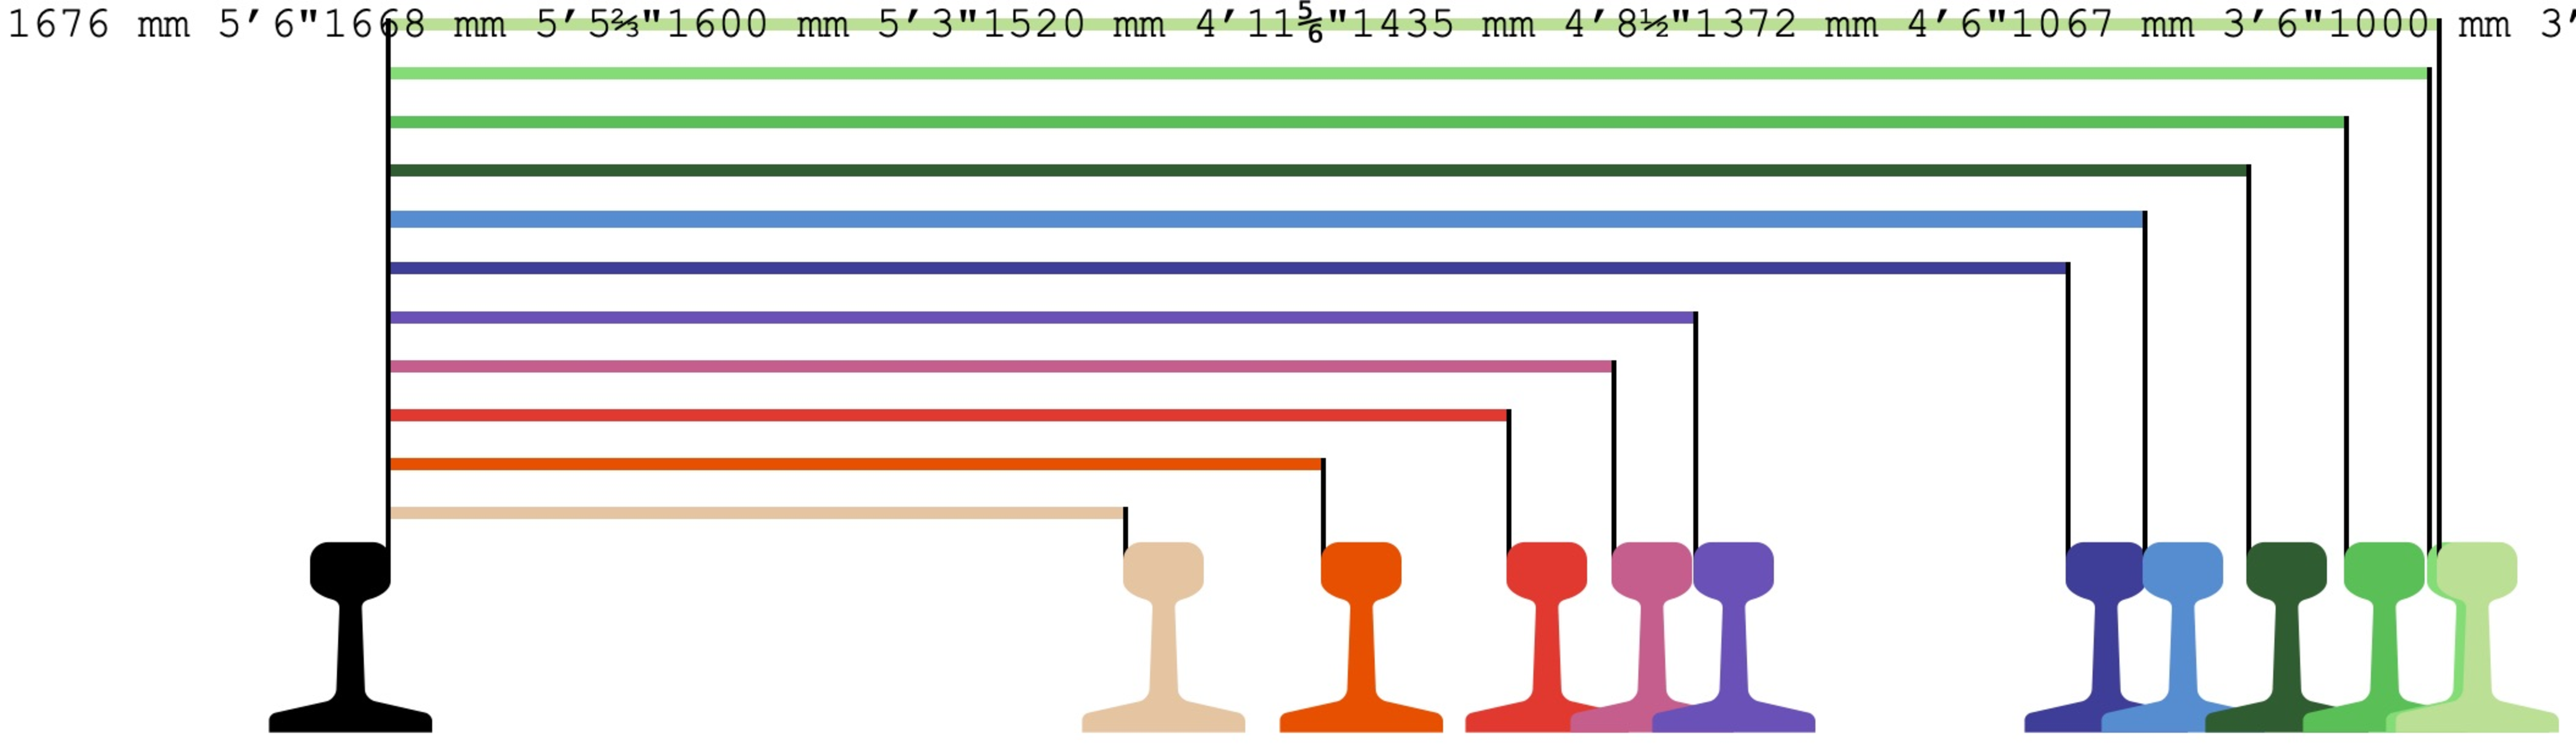
\includegraphics[width=0.7\textwidth]{figures/Track_gauge.pdf}
\caption{軌間}
\label{fig:rail}
\end{figure}

標準は現代世界を支えていますが、しばしば恣意的\is{standard!arbitrary nature of|(}なものです。A4用紙は世界のほとんどの地域で標準であるため、そこではA4がより優れています。USレターサイズは北米の標準であるため、そこではUSレターがより優れています。どちらも本質的に優れているわけではありません。その優位性は、標準であることから来ているのです。

標準英語もこのパターンに従っています。本質的に優れているのではなく、標準であるから優れているのです。他の多くの英語も、もし標準であったならば、標準になり得たのです。

しかし、技術の基準\is{technology standard!vs language standards|(}と言語の基準\is{language standard!vs technology standards|(}には2つの重要な違いがあります。第一に、技術基準は規定されるものです。誰かが計画を立て、それを公表したのです。言語はそのようなものではありません。第二に、技術基準に従わなければ、技術はしばしば機能しません。たとえば、TTCの路面電車は標準軌のレール上では全く走りません。交通手段として使い物にならないのです。同様に、VHSカセットはベータマックスのプレーヤーでは全く再生できません。対照的に、非標準の英語は、標準英語の話者が相手であっても、コミュニケーション\is{communication!and non-standard English}の手段として完全に機能することが多々あります（おそらくほとんどの場合）。私たちが理解できない、あるいは簡単に理解できない方言や変種もありますが、私たちが理解できるものはそれ以上にたくさんあります。コミュニケーションが言語の主な機能であるならば、なぜ私たちは標準英語を持っているのでしょうか？

1つの答えは、言語のもう1つの機能がグループメンバーシップ\is{group membership!and dialect|(}を規定することだということです。言い換えれば、言語は私たちに似ている人、私たちのグループに属している人を特定するのに役立ちます。若者はしばしばスラングを開発し、革新し、使用することで、仲間内のグループ内でアイデンティティや帰属意識を生み出します。たとえば、\enquote{素晴らしい}を意味する形容詞としての \mention{fire} は、一時期、一部の若い話者の間で人気を集めました。そのように使用した人々は、\enquote{私は \mention{fire} のこの新しい意味を知っているグループの一員だ}と宣言しており、さらに\enquote{私はあなたに対してそれを使うから、あなたもそのグループの一員だと思っている}という意味も込めていました。もちろん、大人がそのグループの一部になることはめったになく、大人が \mention{fire} をそのように使うこともめったにありませんでした。

あるいは服装について考えてみてください。カナダのほとんどのカレッジや大学では、ジーンズが標準です。スーツやドレスを着る人もいますが、これらはよりフォーマルではあるものの、依然として標準的な服装の範疇です。教室が暖かければ、上半身裸で現れることも完全に機能的かもしれませんが、それは標準ではありません。人々はそのような服装の選択に対して、驚きや不快感を持って反応するでしょう。スノースーツも非標準ですし、サリー、シェフのユニフォーム、男性のキルトも同様です。キャンパスの人々の中には肯定的に反応する人もいれば否定的に反応する人もいるでしょう。多くの人は表面的な反応を抑えるでしょうが、誰もがこれらの服装が非標準であると認識するはずです。

非標準の英語に関しても同じようなことが言えます。あなたがそれを使えば、人々は気づきます。標準英語は社会的な基準であり、社会的な意味合いを持っています。通常、標準英語を話さない人にとってそれは否定的なものであり、語学教師として、私たちは生徒たちの目標が道具的であると同時に社会的でもあることを認識すべきです。彼らは社会で機能するために英語を学びたいと思っていますが、同時に社会の一部になるために標準英語を学びたいと思っているのです\is{standard!arbitrary nature of|)}\is{technology standard|)}。


\section{標準英語（Standard Englishes）}\label{sec:standard}

ジョージ・エリオットは、彼女の小説『ミドルマーチ』の中で次のような会話を提示しています。

\begin{quote}
    \enquote{All choice of words is slang. It marks a class.}（言葉の選択はすべてスラングだ。それは階級を示している。）

    \enquote{There is correct English: that is not slang.}（正しい英語というものがある。それはスラングではない。）

    \enquote{I beg your pardon: correct English is the slang of prigs who write history and essays. And the strongest slang of all is the slang of poets.}（失礼ですが、正しい英語とは、歴史やエッセイを書く堅物たちのスラングです。そして最も強力なスラングは、詩人たちのスラングです。）
\end{quote}


エリオットは\enquote{正しい英語}と標準英語の違いを知っていました。しかし、多くの人は知りません。残念ながら、私がそれを明確にするために使えるような、標準英語の簡潔な定義\is{Standard English!definition (lack of brief)}はありません（ここでも定義の難しさがあります）。実際、本書の1つの目標は、標準英語の統語論、語彙、および音韻論の限定的な定義を概説することです。しかし、その支配的な地位について、少なくともいくつかコメントすることはできます。

ある程度、英語のどの方言も、あるグループの間では標準ですが、そのほとんどは\enquote{標準英語}とは呼ばれません。もしあなたが標準軌の列車をTTCの地下鉄向けに売ろうとしても、売れることはないでしょう。標準軌はトロントで使用されている標準ではないからです。

もしあなたがファースト・ネーションズ英語\is{dialect!First-Nations English}を話して育ったなら、あなたのコミュニティではファースト・ネーションズ英語がおそらく標準です。あなたのコミュニティに行って標準英語を話す人は誰でも、自らをよそ者として際立たせることになり、良くも悪くもそのように扱われるでしょう。

そして明確にしておきたいのは、標準英語は1つではないということです。カナダ標準英語\is{Standard English!Canadian}、イギリス標準英語\is{Standard English!British}、シンガポール標準英語\is{Standard English!Singapore}などが存在します。大部分において、少なくとも書き言葉にされた場合、これらはほとんど区別がつきませんが、小さな違いはあります。ある変種の独自の特徴は、別の変種の話者にはしばしば目につくものです。それでも、これらはすべて標準英語として、あるいは最近では複数の標準英語として認識されています。

しかし繰り返しますが、これは標準英語が優れているからでも、よりフォーマルだからでも、あるいは最も一般的だからでもありません（特定のコミュニティにおいて最も一般的ではありますが）。\footnote{標準英語が\enquote{何ではないか}についての詳細は、\citet{trudgill99} を参照してください。}\mention{standard} という言葉は、\mention{grammatical} や \mention{correct} の同義語ではありません。真実、論理、美しさ、純粋さ、あるいは明晰さを暗に意味するものでもありません。それは英語がどのように話される\enquote{べき}かということではありません。それは単なる方言の集まり\is{Standard English!as a cluster of dialects}であり（強力なものではありますが）、英語話者の支配的な社会的グループによって施行されている規範に過ぎないのです。世界の多くの地域で、それはイギリスや、先住民が大部分追いやられた旧イギリス植民地（例：カナダ）の教育を受けた英語話者を意味しますが、先住民が追いやられなかった場所（例：バングラデシュ）の話者は含まれません\is{Standard English!not inherently superior|)}\is{dialect!and Standard English|)}。

\begin{tblsframed}{\term{シボレス（shibboleth）}\is{shibboleth|(}とは何か？} \label{sec:shibboleth}
    ヘブライ語聖書の7番目の書である士師記には、方言の門番としての機能\is{shibboleth!gate-keeping function}に関する物語があり、次のような内容です。

    \begin{quote}
        エフタはギレアデのすべての人を集めてエフライムと戦った。ギレアデの人々はエフライムを打ち破った。エフライムが、\enquote{あなたがたギレアデは、エフライムとマナセの間にあるエフライムの逃亡者だ}と言ったからである。
        ギレアデはエフライムへ行くヨルダン川の渡し場を攻め取った。エフライムの逃亡者が、\enquote{渡らせてくれ}と言うと、ギレアデの人々は、\enquote{おまえはエフライム人か}と問い、彼が\enquote{違う}と答えると、
        彼らは、\enquote{それでは \mention{Shibboleth}（シボレス）と言ってみろ}と言った。彼がそのとおりに正しく発音できず、\enquote{Sibboleth}と言うと、彼らは彼を捕らえ、ヨルダン川の渡し場で彼を殺した。その時、エフライムは四万二千人倒れた。 --士師記 12:4-6 (新改訳聖書をもとに調整)
    \end{quote}

    \indent この物語から、英語の \mention{shibboleth}\is{shibboleth!origin of term} という言葉が生まれました。これは特定のグループの人々を区別する話し方であり、しばしばアイデンティティの確認や帰属のテストとして使用されます。\mention{shibboleth} という用語は現在、\enquote{インサイダー}と\enquote{アウトサイダー}を分けるあらゆる種類の言語的または文化的指標を意味します。現代の用法において、シボレスは生と死の問題ではないかもしれませんが、それでも私たちが他者をどのように認識し、どのように接するかに大きな影響を与える可能性があります。

\end{tblsframed}

\section{文法性への問い} \label{sec:questioning-grammaticality}

私が初めて英語教師として雇われたとき、それは私の資格のせいではありませんでした。私には何の資格もありませんでした。また、経験のせいでもありませんでした。先ほど言ったように、それが私の最初の教職だったからです。それでも、私が日本に到着したとき、2週間以内に雇われました。これはおそらく私が標準英語の\enquote{ネイティブスピーカー}であったからだと推測しています。白人であることもおそらく役立ったのでしょう。

標準英語を話して育った人間として、私は明らかにこの言語の有能な使い手でしたが、明示的な文法知識はほとんど持っていませんでした。カナダのほとんどの学校は、英文法について本質的に何も教えません。それは私が学生だった頃もそうでしたし、現在でもそうです。私はフレンチ・イマージョンの初期の波の中にいたため幸運でした。少なくとも（フランス語の）文法について何かを知っていたからです。しかし、生徒たちの質問に答えようとしたとき、それはほんのわずかな助けにしかなりませんでした。

\enquote{なぜここでは現在進行形を使い、あちらでは現在形を使うのですか？}、\enquote{いつ \mention{the} が必要ですか？}、\enquote{なぜ \mention{who \emph{does} she know} とは聞くのに、通常 \mention{who \emph{does} know her} とは聞かないのですか？}これらのすべての質問に対して、私は\enquote{そう言う方が自然に聞こえるから}以上のことはほとんど言えませんでした。私は何が文法的で何が非文法的かについて強い直感\is{intuition!about grammaticality}を持っていましたが、それらの直感を体系的かつ一般化可能な方法で生徒たちに伝える術を持っていませんでした。そもそも、何かが文法的であるとはどういう意味なのかについて考えたことすらありませんでした。

この時点で、あなた（そうです、あなたです）は、かつての私よりもずっと多くの英語文法の明示的な知識をすでに持っています。実際、あなたはおそらく平均的な大学教授よりも英文法に関する明示的な知識を持っています。もし生徒が \mention{I had coffee and a piece of toast for breakfast} の中の限定詞について尋ねてきたら、\mention{coffee} は不可算名詞なので限定詞を必要としないが、単数の可算名詞である \mention{piece} は限定詞なしでは使えないと教えることができるでしょう（セクション~\ref{sec:count} を参照）。あなたは英文法について何かを知っています。ですから、私が始めた頃よりもずっと先を行っているのです。

しかし、あなたもまた、何かが文法的であるとはどういう意味なのかについて考えたことがないかもしれません。これがここで探求したいことです。（より完全な扱いは第\ref{ch:grammaticality}章で行います。）

\begin{tblsframed}{\term{単義性の誤謬（The fallacy of monosemy）}\is{fallacy of monosemy|(}} \label{sec:fallacy-of-monosemy}\is{monosemy}
    しかし、本題に入る前に、単義性の誤謬について一言述べておきます。もしある単語が単義的であれば、それは単一の（\mention{mono--}）意味（\textit{\emph{sem}antics}）を持っています。これは、子供が\enquote{\mention{can I go to the toilet}}と尋ねたときに、教師が意地悪く\enquote{\mention{I don't know, \emph{can} you?}}と答えるときに働いている考え方です。教師は \mention{can} が\enquote{能力}というたった1つの意味しか持たないかのように振る舞っていますが、実際には \mention{can} は複数の意味を持っています。第1章で、専門的な意味と日常的な意味について触れました。誰かが\enquote{専門的にはその単語は $x$ を意味する}と言うとき、単にその単語の専門的な意味合いが存在すると言っているだけかもしれませんが、多くの場合は単義性の誤謬に陥っているのです。
\end{tblsframed}\label{sec:monosemy}

\mention{grammatical} という言葉にたった1つの真の意味があると見せかける必要はありませんが、だからといって何でも意味するわけではありません。\mention{grammatical} の意味をどのように確立するのでしょうか？図~\ref{fig:comic} のコミックが説明しているように、言葉が何を意味するかは、私たちがそれを使うときに何を意味するかに依存しています。

ですから、あなたにとって \mention{grammatical} と \mention{ungrammatical} が何を意味するのか少し時間をかけて考えてみてください。あなたがこれらの言葉を使ったときのことを思い出してください。あなたは何を指していましたか？もし思い浮かばなければ、それぞれの例を作ってみてください。いずれにせよ、他の例にも一般化できるかもしれない共通点を考えてみてください。特に境界事例が思い浮かんだ場合は重要です。

\begin{figure}
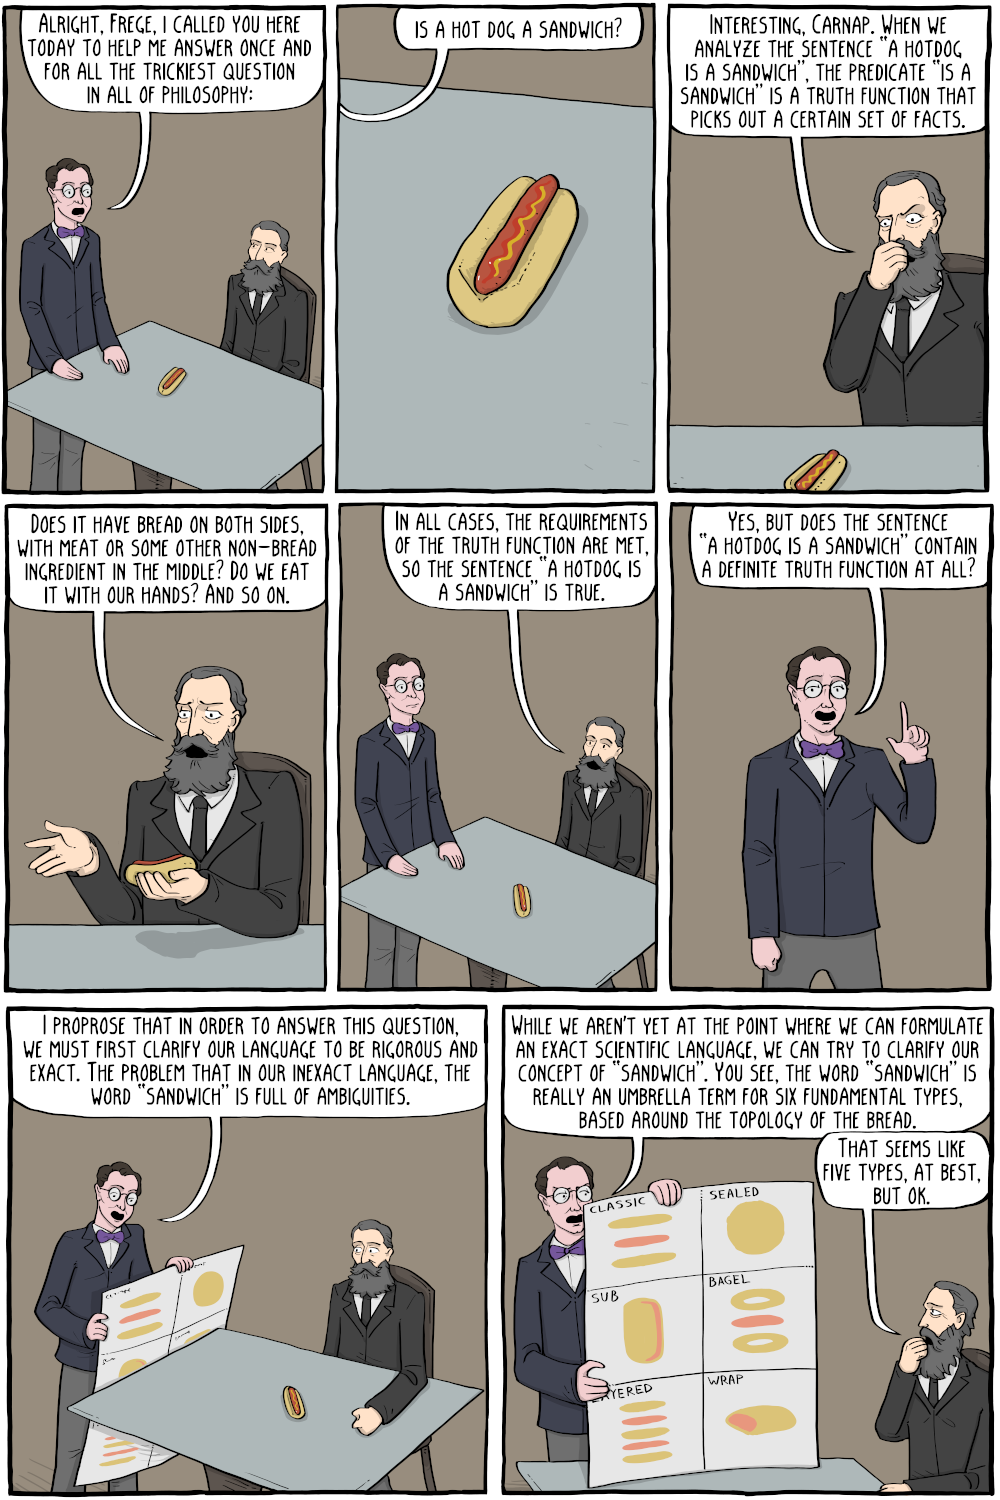
\includegraphics[width=0.95\textwidth]{figures/hotdogSandwich1.png}
\end{figure}

\begin{figure}
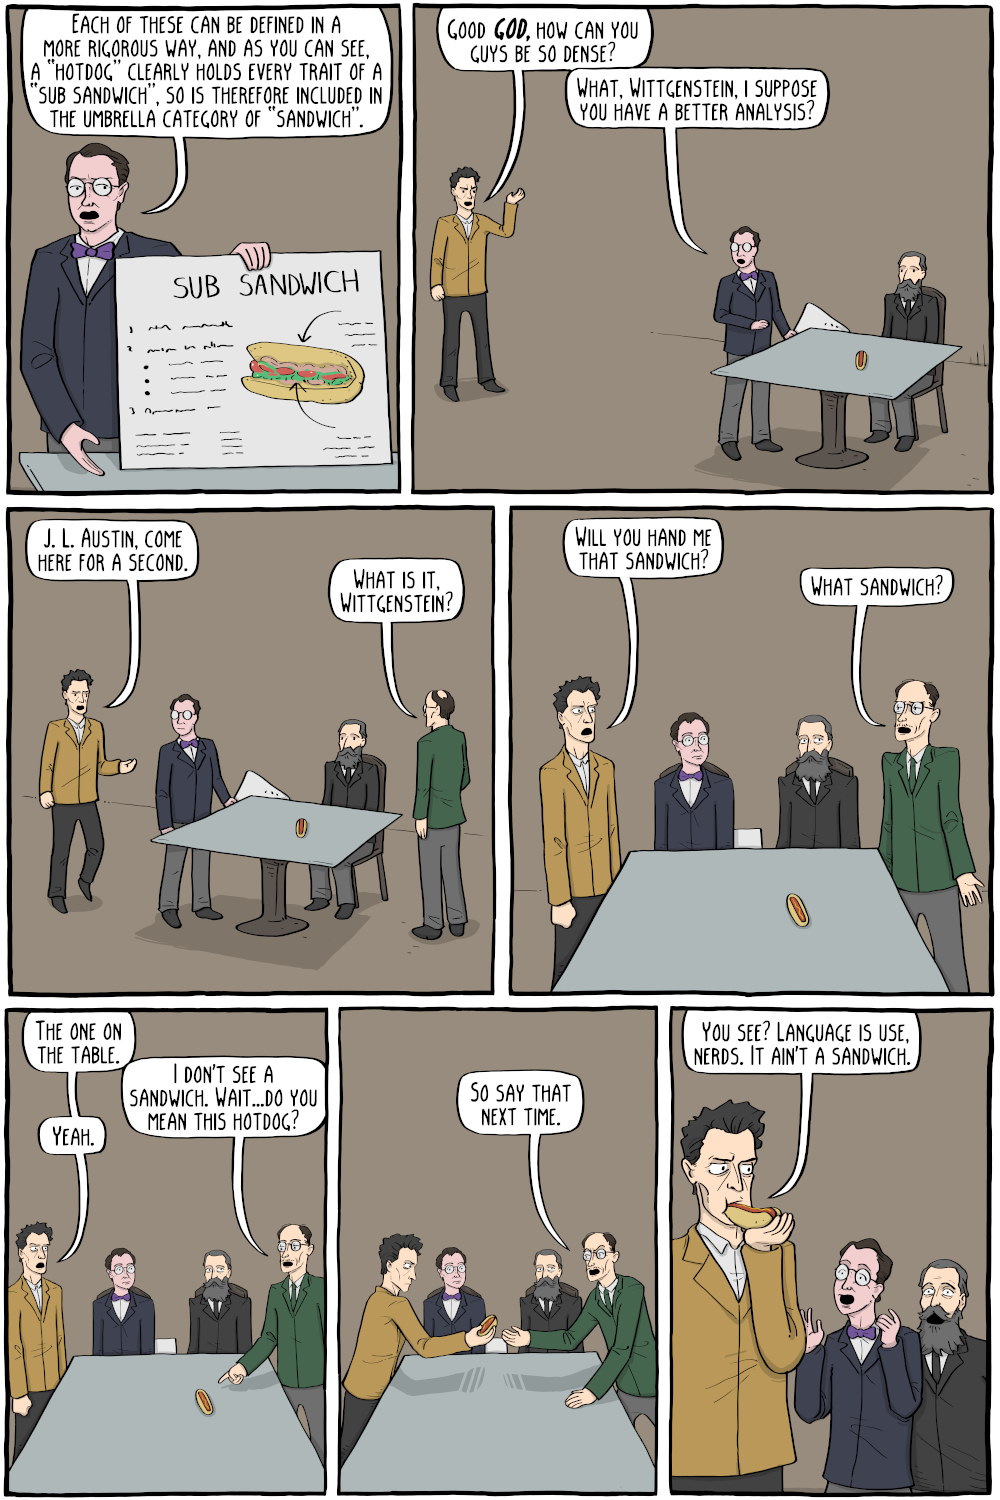
\includegraphics[width=0.90\textwidth]{figures/hotdogSandwich2.png}
\caption{Is a Hotdog a Sandwich? A Definitive Study, from \textit{Existential Comics} by Corey Mohler.}
Source: \url{https://existentialcomics.com/}
\label{fig:comic}
\end{figure}

\textit{The concise Oxford dictionary of linguistics} \citep{Matthews2003} では、\mention{grammatical} を次のように定義しています。


\begin{enumerate}[noitemsep]
    \item 文法に関すること [\dots]。
    \item 特に、ある言語の規則に従っている文などについて。例：英語において \mention{I like tea} は文法的であるが、\mention{I tea like} は非文法的である。したがって、文法性\is{grammaticality!definition}は、特定の文法によって文に割り当てられる特性、あるいはその文法を仮定的に\enquote{知っている}話者によって容認可能であると判断される文の特性のいずれかである。
\end{enumerate}

言語とは単なる使用であるというウィトゲンシュタインの概念に行き着くのでしょうか？私たちが話すことはすべて文法的であるということでしょうか？私たちの発話が私たちの文法を定義するのでしょうか？まあ、そうですが、それはあなたやあなたの生徒の役には立たないので、いくつかの例を考えてみたいと思います。

簡単なものから始めましょう。


\ea[]{Me key there happy mine the.}
\label{ex:key}
\z
(\ref{ex:key}) が紛れもなく非文法的\is{ungrammaticality!example of|(}であることに同意していただけると思います。しかし、なぜでしょうか？いや、本当に、なぜでしょうか？もしあなたがこれが非文法的だと感じるなら、その直感を裏付けるために何を指摘できますか？もし誰かがこれが実際には文法的だと主張したら、私たちはどのような反論ができるでしょうか？

さて、\mention{key} から始めて、それが単数の可算名詞であるため限定詞が必要であり、それがないように見えると言えるかもしれません（セクション~\ref{sec:count} を参照）。\mention{my} のようなNPは限定詞として機能できますが、少なくとも標準英語において \mention{me} はそのようには機能しません。おそらくこれは \mention{me} が\enquote{私の}を意味する別の方言の \mention{me} かもしれませんが。あなたは \mention{key} を見て、それが名詞なのか動詞なのかを自問するかもしれません。もしそれが名詞なら、動詞はありません。そしてもしこれが節であるべきなら、主要部としてVPが必要です（セクション~\ref{sec:verbs} を参照）。そこで、\mention{key} が動詞だと仮定しましょう。そうなると \mention{me} が主語になりますが、ここでは \mention{me} ではなく \mention{I} が期待されます。そして \mention{key} が動詞なら、あなたは何かをキーで傷つける（key something）ことを期待します。残念ながら、\mention{there} と \mention{happy} はキーで傷つけられる\enquote{何か}ではありません。\mention{please key mine} と言うことはできますが、それが機能するためには \mention{mine} が \mention{key} から離れすぎているように思えます。そして \mention{the} は、通常決して現れない位置である文末に残されています。

私は続けることができますが、おそらくもっと単純なことです。もしかすると (\ref{ex:key}) は意味をなさないから非文法的なのかもしれません。文法的な言語は常に意味をなすものなのでしょうか？意味をなすものは文法的だと言えるでしょうか？（これらは同じ主張ではありません。）批判的思考を持つ者として、私たちは自分のアイデアを反証しようとする必要があります。意味をなさない文法的な発話を作成し、非文法的な発話と比較することでこれを行うことができます。幸いなことに、言語学において非常に影響力のあるノーム・チョムスキーが、(\ref{ex:greenIdeas}) の有名な（少なくとも言語学においては）例でそれをすでに行ってくれています。

\ea
    \ea[]{Colorless green ideas sleep furiously.}
    \label{ex:greenIdeas1}
    \ex[*]{Furiously ideas sleep green colorless.}
    \label{ex:greenIdeas2}
    \z
    \label{ex:greenIdeas}
\z

\begin{figure}
    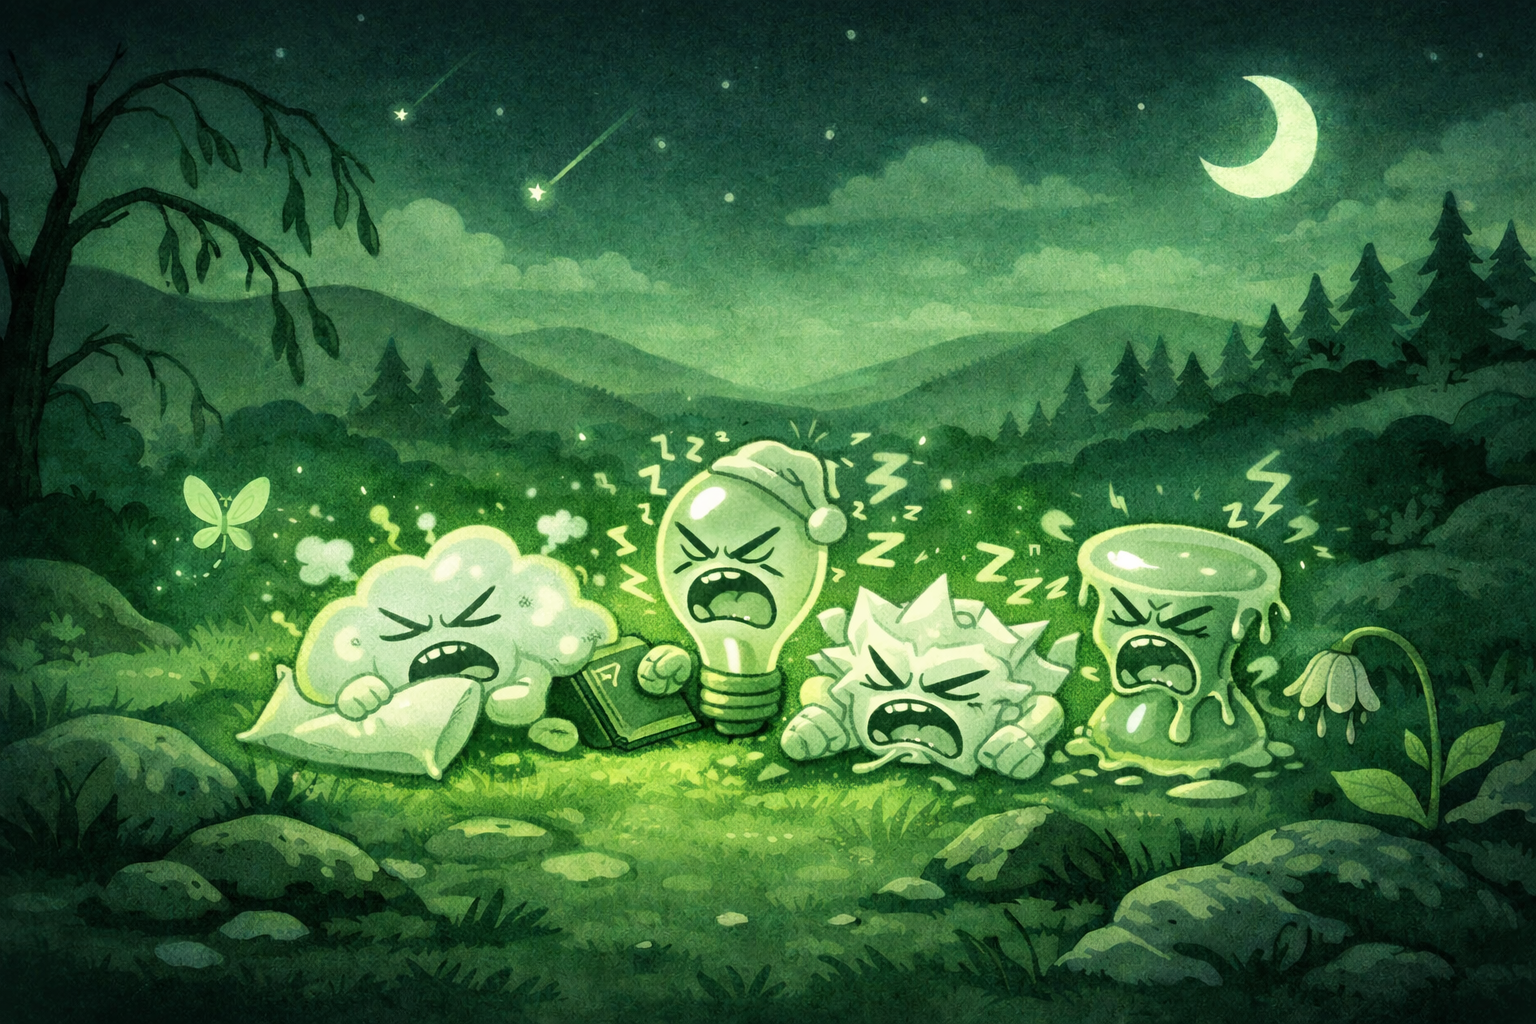
\includegraphics[width=3in]{figures/green-ideas.png}
    \caption{Colorless green ideas sleep furiously.}
    \label{fig:greenIdeas}
\end{figure}

\textcite[16]{Chomsky2002-ko} は、(\ref{ex:greenIdeas1}) は文法的であり、(\ref{ex:greenIdeas2}) は非文法的であると主張しています。これは私の直感と一致します（あなたの直感とも一致すると思います）。文法的であるために意味をなす必要はないようです。


しかしチョムスキーはまた、これらの文やその部分が英語のコーパスに出現することはなく、\enquote{英語のいかなる統計モデルにおいても、英語から同等に『かけ離れて』いる}と主張しています。彼は、頻度は関係ないと言いたいのです。ここにおいて、彼は間違っていると思います。フェルナンド・ペレイラ（Fernando \textcite{Pereira2000}）は、(\ref{ex:greenIdeas1}) が実際には (\ref{ex:greenIdeas2}) よりも統計的にずっと起こりやすいことを示しました。そして ChatGPT のような大規模言語モデルの成功は、言語が統計的規則性\is{grammaticality!and statistics}の上に構築されていることを真に示しています \citep{Kallini2024}。

次に、その逆である、有意味な言語はすべて文法的であるということを検討します。それを行う前に、非文法的であるが明確な意味を持つものを何か考えてみてください。

さて、(\ref{ex:JeanPaul}) を考えてみてください。

\ea[]{Jean Paul, very very good.}
\label{ex:JeanPaul}
\z
この例は私の友人であるジェフ・プラムがNPRのインタビューで聞いたものです。話者はトルコ人でした。その文脈における彼女の意味は明らかに、教皇ヨハネ・パウロが非常に、非常に良い教皇または人物であったということでした。しかし、これが英語で文法的であるためには、主語と主要部を持つ節が必要です。その主要部はVPであるべきで、つまり動詞が必要になります。おそらく \mention{be} でしょうが、\mention{seem} や \mention{become} のような叙述補語を認可する他の動詞も可能でしょう。

つまり、何かが文法的であっても意味をなさない\is{grammatical!vs meaningful}ことがあり、意味をなすけれども文法的ではない\is{meaning!and grammaticality|(}ことがあるようです。したがって、意味は文法性のための必要条件でも十分条件でもありません。\is{necessary and sufficient conditions}

それでは、別の考えです。おそらく私たちは文法書の規則\is{grammaticality!and rule books}にただ従えばいいのではないでしょうか。

\ea
    \ea[]{He was a beautiful young man, a beautiful beautiful boy.}\label{ex:beautifulboy}
    \ex[*]{The boy was beautiful beautiful.}\label{ex:beautifulboy2}
    \z
\z
星印（*）でわかるように、私は (\ref{ex:beautifulboy}) は文法的だと思いますが、(\ref{ex:beautifulboy2}) はそうではないと思います。あなたも同意してくれると思います。これを説明する規則は \textit{CGEL} (p. 561) にあり、私の知る限り \textcite{Watt1968} によって最初に注目されました。しかし、それは広く知られておらず、あなたもこれまでに遭遇したことはないと思います。また、(\ref{ex:beautifulboy}) と (\ref{ex:beautifulboy2}) の文法性が、Watt が論文を書いたときから \textit{CGEL} が出版されるまでの間に変わったわけでもないと仮定します。これらのことを考慮すると、文法書の規則が何が文法的かを規定するという考えは脇に置いておくことができるでしょう。多くの規則は文法書に言及されていません。実際、言語学者がそのための文法書を一切書くことなく存在している言語がたくさんあります。本が書かれていないからといって、それらの言語では何でもありだと言いたくはないはずです。

さて、(\ref{ex:whmovement}) を考えてみてください。

\ea[*]{What movies do you have friends who acted in?}
\label{ex:whmovement}
\z
おそらくこれは非常に奇妙な文で、文法的であると同時に非文法的であるように感じる、まるで目の錯覚のような文だということに同意するでしょう。その理由は、\term{島の制約（island constraints）}\is{island constraint}と呼ばれるものによる結果だと考えられています。これは、これに関して議論はありますが、多くの言語学者がすべての言語に適用されるかもしれないと考えている一種の規則または制限です。これは私たちの脳の処理の制約\is{processing limitations!and grammaticality|(}による結果である可能性もありますし、情報がどのように構造化されるかに関する何かである可能性もあります。幸いなことに、もしこれが真実であれば、あなたはこれを生徒に説明する必要は決してないでしょう。なぜなら、誰も素朴にこのような文を使おうとはしないからです。

つまり、私たちの処理能力が、何が文法的で何がそうでないかを判断するのに役立っているようです。これを念頭に置いて、(\ref{ex:suitcase}) が図~\ref{fig:suitcases} のどちらの画像を説明しているか考えてみてください。

\ea[]{After the trip, my suitcase sat unpacked on the floor for days.}
\label{ex:suitcase}
\z

\begin{figure}
    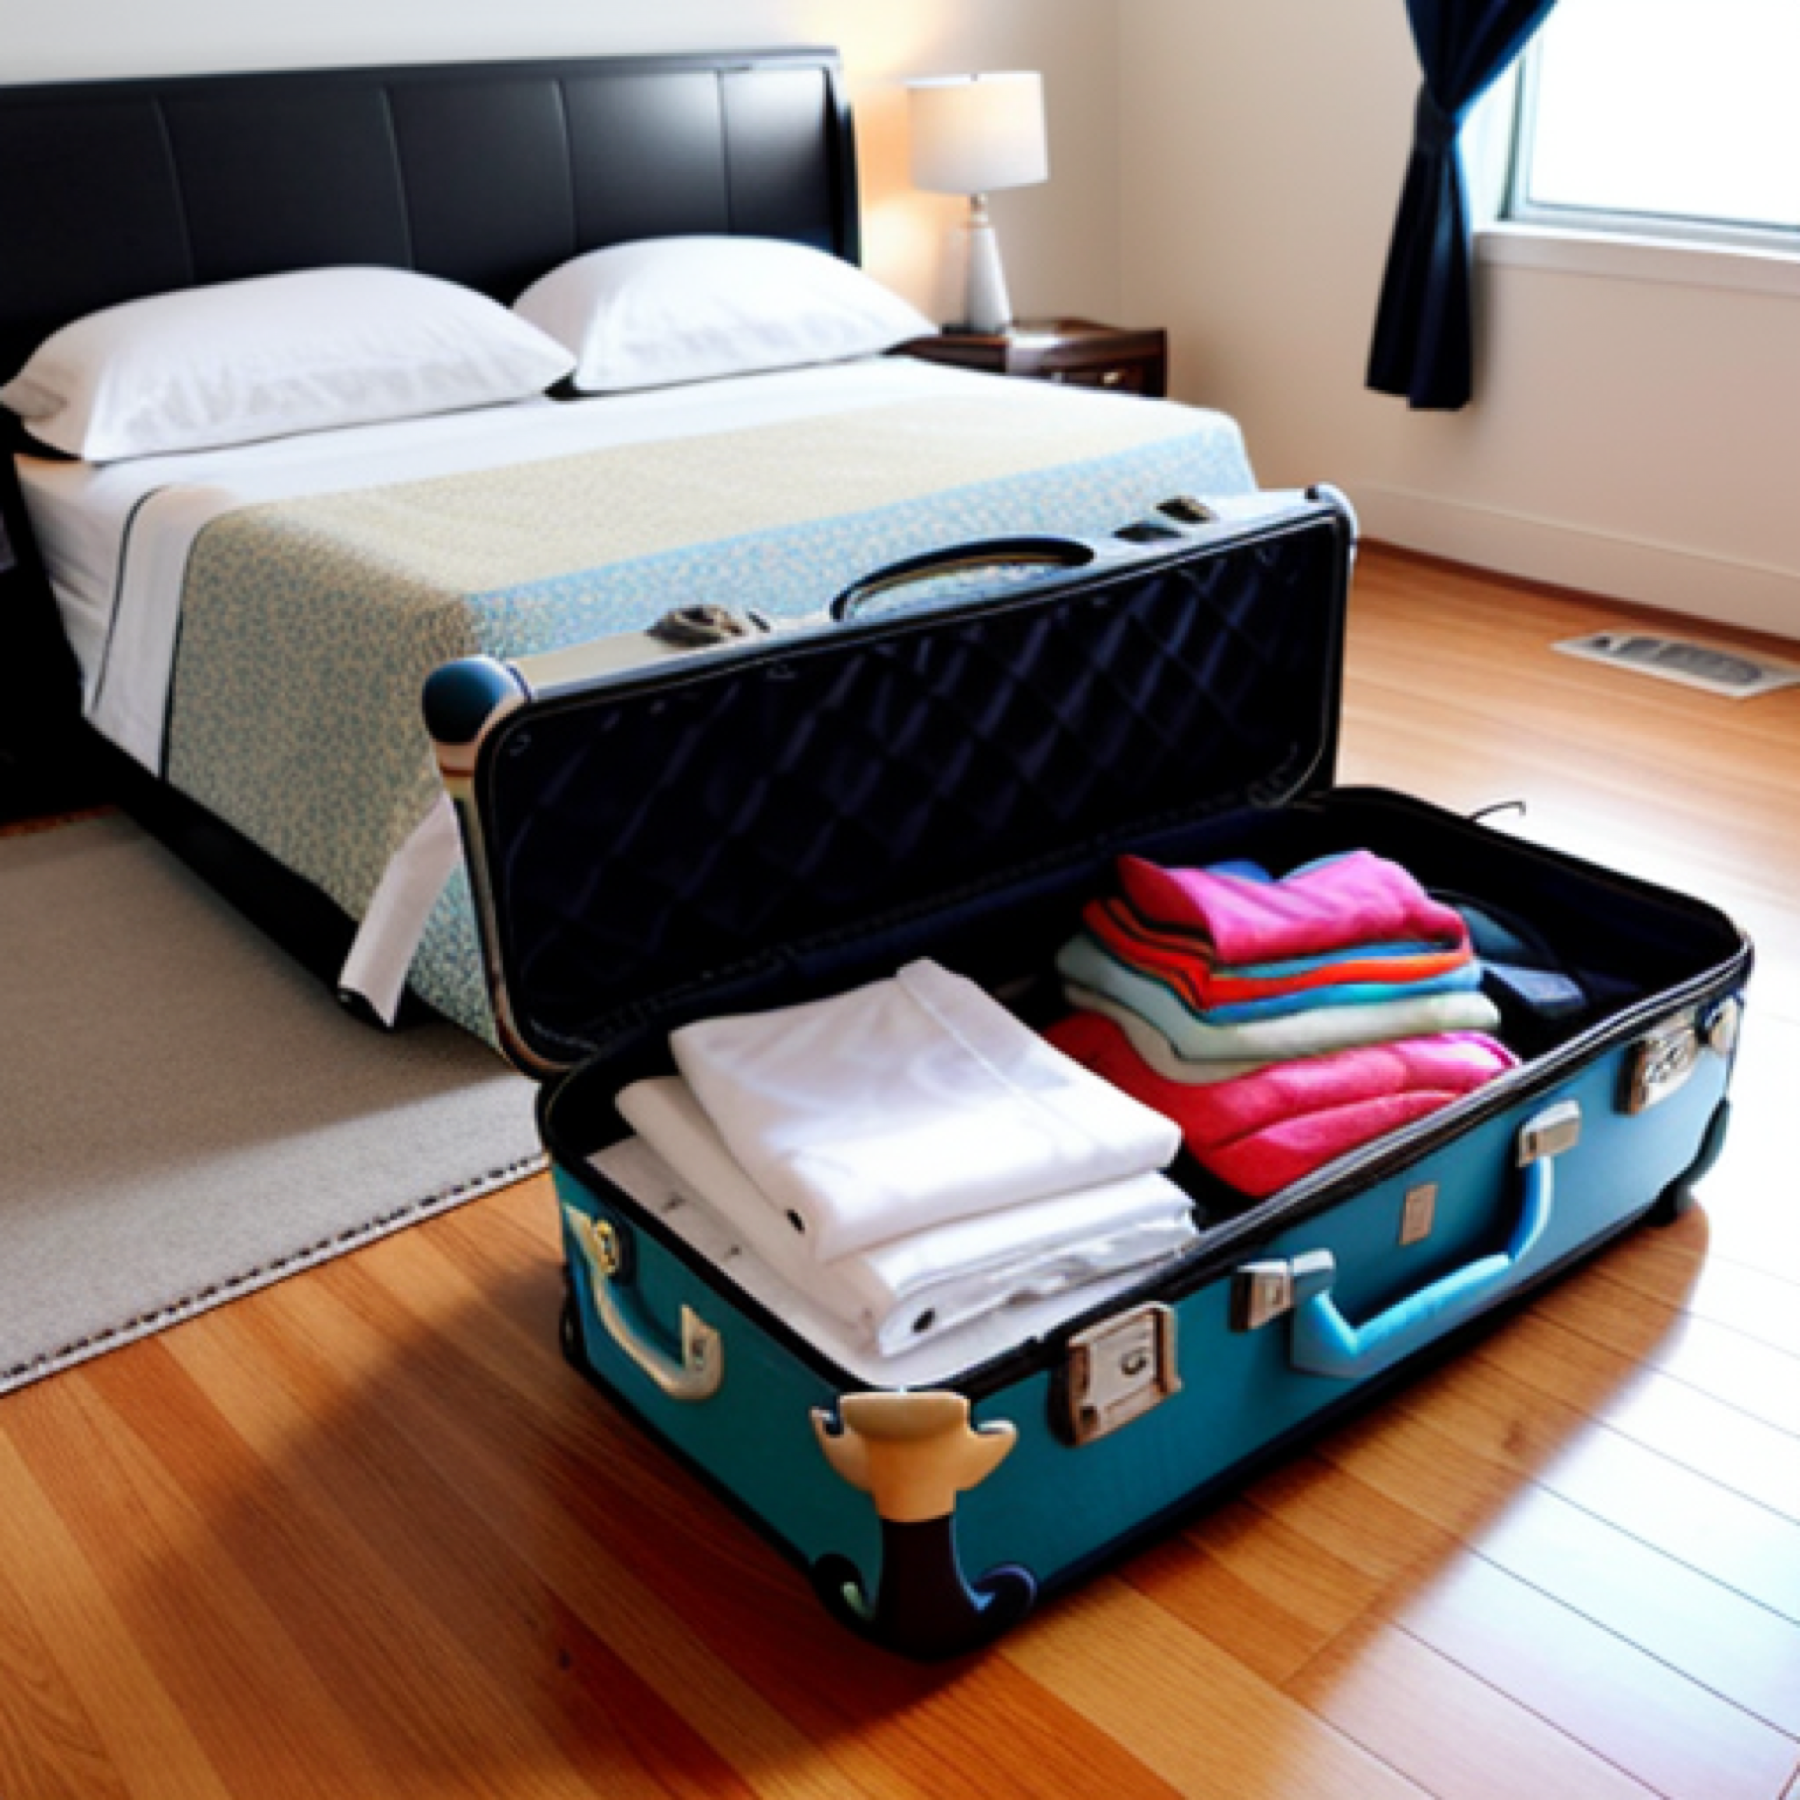
\includegraphics[width=2in]{figures/full_suitcase.png}
    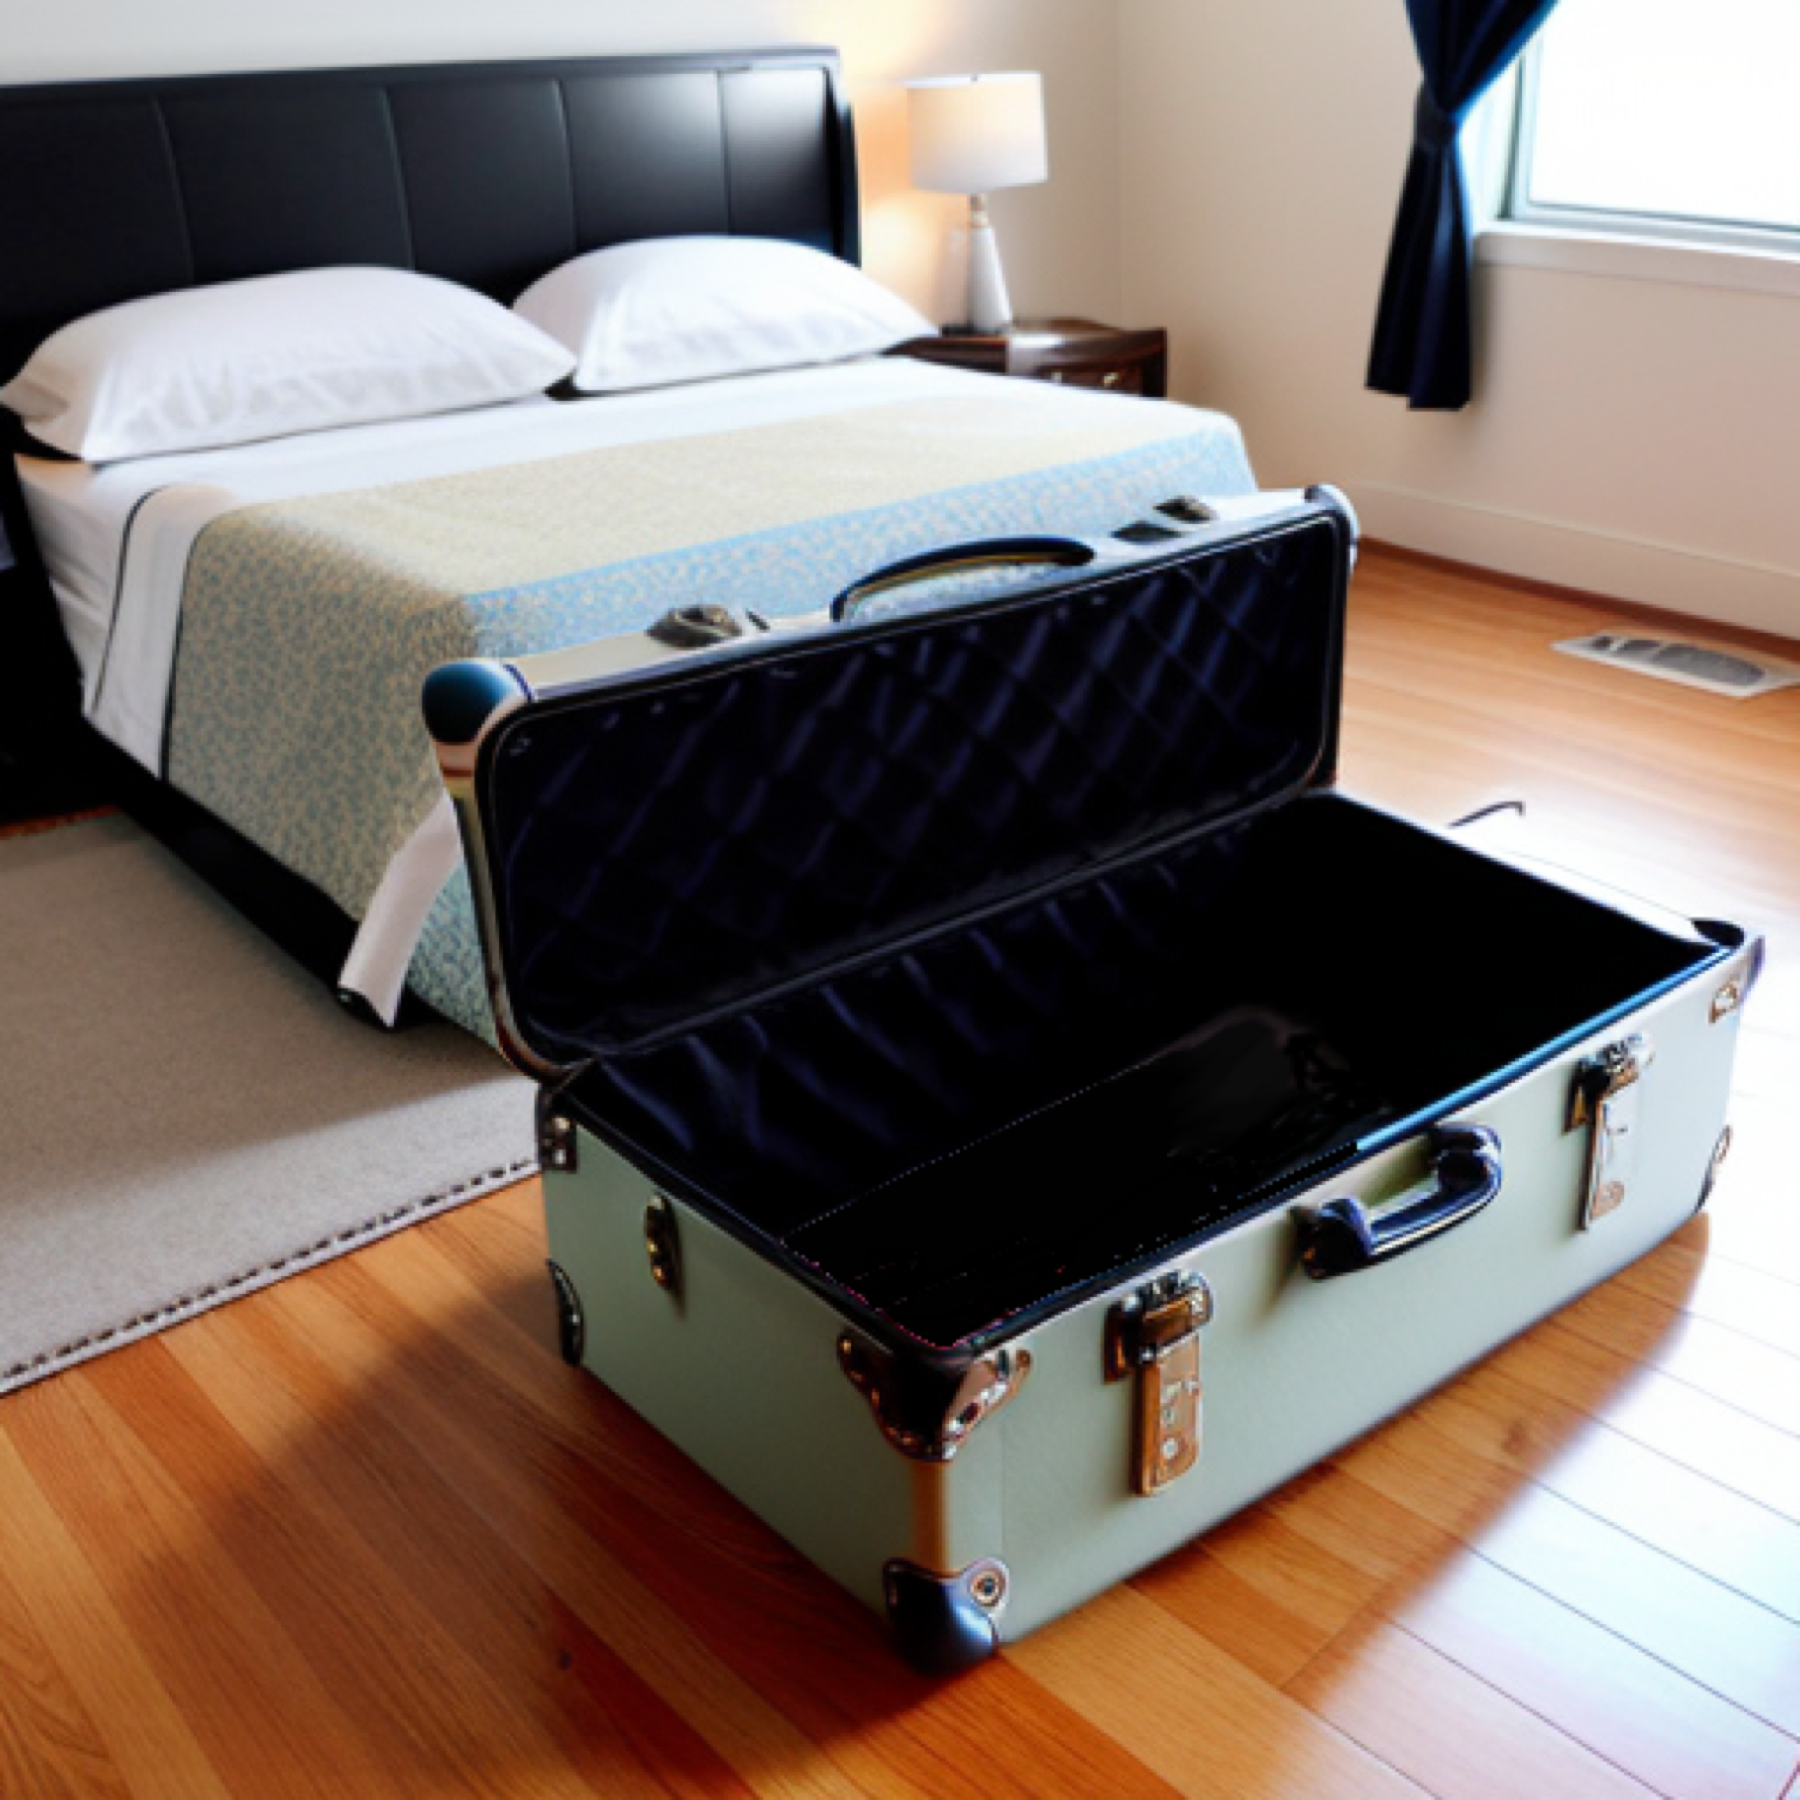
\includegraphics[width=2in]{figures/empty_suitcase.png}
    \caption{どちらのスーツケースが unpacked ですか？}
    \label{fig:suitcases}
\end{figure}

多くの人は、これは最初のスーツケース（左側の服が入っているもの）だと言いますが、それは間違いです。最初のスーツケースは \mention{packed} です。スーツケースを \mention{pack} するとき、あなたは服を中に入れます。2番目のものは \mention{unpacked} されています。すべての服が取り出されているのです。

なぜ人はこれを間違えるのでしょうか？この問題について考えた人々は、否定、つまり \mention{unpacked} の先頭にある \mention{un--} に何か巧妙な罠があると感じることがよくあります。結局のところ、それを \mention{packed} に置き換えれば、意味は完全に明確になります。では、私たちの言語処理の方法に、時折私たちの理解を混乱させるある種のバグがあるのでしょうか？もしかすると、何が文法的かを判断するために直感に頼ることは全くできないのかもしれません。実際、これはまさに (\ref{ex:horse}) が示唆していることです。

\ea[]{The horse raced past the barn fell.}
\label{ex:horse}
\z
言語学で有名なもう1つの文である (\ref{ex:horse}) は、おそらくあなたには非文法的に思えると思いますが（\citet{bever1971} より）、星印（*）がないことにお気づきかもしれません。\mention{raced} を \mention{ridden} に変えたらどうでしょうか？今度は明らかに文法的です（もし明確でなければ、これは\enquote{納屋を通り過ぎて走らされたその馬は転んだ}という意味です）。あなたが (\ref{ex:horse}) で抱えた問題は、\mention{raced} を過去分詞形（\mention{ridden} のような）ではなく、過去形（\mention{rode} のような）として解釈したことでした。やはり、私たちの直感は100\%信頼できるわけではないのかもしれません。時として、一歩一歩慎重に考え抜く必要があります。

(\ref{ex:30years}) に関して言えば、これは完全に文法的であるように私には思えます（比較：\mention{I have 30 dollars}）。実際、多くの言語において年齢はこのように語られます。しかし、それが文法的であったとしても、少なくとも英語において \mention{I'm 30 years old} と言う方法としては間違っています。ですから、文法的であることさえも、容認可能\is{grammatical!vs acceptable}であることと同じではないのです。
\ea[\textsuperscript{?}]{I have 30 years.}
\label{ex:30years}
\z
北米の英語話者は一般的に (\ref{ex:weekend}) を非文法的だと判断しますが、これはイギリス英語において \mention{I'll see you on the weekend} を表現する通常の方法です。

\ea[\textsuperscript{!}]{I'll see you at the weekend.}
\label{ex:weekend}
\z
これはセクション~\ref{sec:standard}で触れた、標準英語間の小さな違い\is{Standard English!regional differences}の1つであり、\enquote{!}のマークはそれが標準英語の変種間で異なることを示しています。この違いの理由は文法的なものではなく、週末に関する関連するメタファー\is{metaphor!for weekend (platform vs point)}について異なる文化的前提の下で操作しているためです。北米人は週末を出来事が展開するプラットフォームや舞台として捉えているのに対し、イギリス人は週末を週の終わりにある点として見ていると主張されています。\footnote{メタファーと前置詞についての詳細は、セクション~\ref{sec:preposition-meanings} を参照してください。}

\ea[\textsuperscript{\%}]{I ain't no quitter.}
\label{ex:quitter}
\z
(\ref{ex:weekend}) とは異なり、(\ref{ex:quitter}) は標準英語間の違いではありません。\enquote{\%}のマークは、標準英語では文法的ではないかもしれないが、他の変種では文法的である形式を示しています。

\ea[]{Me and Mia are taking the bus.}
\label{ex:bus}
\z
対照的に、(\ref{ex:bus}) はすべての方言において完全に文法的ですが、インフォーマルな使用域\is{style restrictions (formal, informal, etc.)!and register}に属しています。よりフォーマルなバージョンでは \mention{Mia and I} を使用します。これは一部の人々にとってのシボレス\is{shibboleth!example of}です。

最後に、私が非文法的だと感じる (\ref{ex:bad-and}) を修正してみてください。
\ea[*]{Jim and me's teacher was Geoff.}
\label{ex:bad-and}
\z
ここには良い解決策がありません。もしそれを \mention{Jim and my} に変えれば、それは\enquote{私の先生とジム}のようになり、私が意味していることではありません。\mention{me and Jim's} にも同様の問題が当てはまります。しかし、*\mention{Jim and my's} は *\mention{Jim and me's} と同じくらい非文法的に聞こえます。特定の単純な概念を表現するために、時には非文法的である必要があるのかもしれません。私はそうしたケースがあるかもしれないと考えています\is{ungrammaticality!example of|)}\is{fallacy of monosemy|)}\is{intuition!about grammaticality|)}\is{meaning!and grammaticality|)}\is{processing limitations!and grammaticality|)}\is{grammaticality!questioning of|)}\is{grammatical!vs meaningful|)}。

\subsection{まとめ}

一般的に、文法的なものは意味をなし、その逆もまた然りですが、意味をなすことは文法性のための必要条件でも十分条件でもありません。規則の多くは文法書に記述されていますが、多くは記述されていません（そしてしばしば文法書の記述は間違っています）。英語の熟練した使用者は、何が文法的かを知るために概ね直感に頼ることができますが、私たちの直感は騙されることがあります\is{intuition!fallibility of|(}。時には、説明が以前には見えなかったものを見るのに役立つこともあります。文法的なものでも私たちが言わないようなことがあり、また文法的に言うことができないこともあります。それでは、文法的なものを文法的にしているのは何でしょうか？

\section{文法性のモデル} \label{sec:gramm-model}

さて、文法性は私たちが思っていたほど単純ではないことを見てきました。しかし、だからといって文法性について有用な考え方ができないというわけではありません。役立つかもしれないモデル\is{grammaticality!model of|(}をここに示します。

その核心において、文法性とは、特定の状況における特定のスピーカーグループに対して機能する形式と意味のペアリング\is{form--meaning!pairing|(}に関するものです。それは普遍的なものではありません。図~\ref{fig:speaker_groups} は、それらのグループのほんの一部を示しています。私が言いたいことを理解するために、10代の若者が\enquote{それはあなたのお母さんの靴下だ}という意味で \mention{mommy sock} と言うことを考えてみてください。これは非常に非文法的に（そして非常に奇妙に）感じられます。しかし、幼児による同じ発話は、どちらの感情も呼び起こしません。なぜなら、それは特定の状況における特定のスピーカーグループに対して機能する、適切な形式と意味のペアリングだからです。

あるいは、\citet[179]{nishimura1995} からの次の会話を考えてみてください。斜体のテキストは日本語\il{Japanese}で、単一引用符の中に翻訳があります。

\begin{quote}
    B.C. \mention{ni iku toki} (`When I went to B.C.'), \mention{hikōki de yomoo to omotte kara} (`thinking I would read it on the plane'), I bought it, eh? So, it's not finished yet. (Laughs) And it's hard, 'cause me\mention{-nanka} (`a person like me'), \mention{mō} (`really'), \mention{hon-nanka yomu to} (`when I read a book'), cover-to-cover \mention{yomanakattara} (`unless I read it cover-to-cover'), if I stop \mention{dokka de }(`at some point'), I forget the story.\\
    （B.C.に行く時、飛行機で読もうと思ってから、買ったのね。だから、まだ終わってないの。（笑）そして難しいの、だって私なんか、もう、本なんか読むと、カバーからカバーまで読まなかったら、どっかで止めたら、話を忘れちゃうの。）
\end{quote}

このような\term{コードスイッチング（code-switching）}\is{code-switching!and grammaticality}\is{code-switching!example of}は、英語と日本語のバイリンガルにとっては完全に文法的ですが、他の英語話者にとっては大部分が非文法的に思えます。

\begin{figure} \label{fig:speaker-groups}
\begin{tikzpicture}[scale=0.8]
    % Main ellipse for all English speakers
    \draw[fill=white, thick] (0,0) ellipse (7cm and 5cm);
    \node[align=center] at (0,4.2) {All English Speakers\\（すべての英語話者）};

    % Ellipse for Standard English speakers
    \draw[fill=white, thick] (-1,0) ellipse (5cm and 3cm);
    \node[align=center] at (-1,2.3) {Standard English Speakers\\（標準英語話者）};

    % Smaller ellipses for different groups
    \draw[fill=white, thick] (-3,-1) circle (1.2cm);
    \node[align=center] at (-3,-1) {Teachers\\（教師）};

    \draw[fill=white, thick] (0,-2) circle (1.2cm);
    \node[align=center] at (0,-2) {Teens\\（10代）};

    \draw[fill=white, thick] (2.7,0.9) circle (1.3cm);
    \node[align=center] at (2.7,0.9) {Singaporeans\\（シンガポール人）};

    \draw[fill=white, thick] (4,-2) circle (1.2cm);
    \node[align=center] at (4,-2) {Infants\\（幼児）};

    \draw[fill=white, thick] (-4.2,1.3) circle (1cm);
    \node[align=center] at (-4.2,1.3) {Lawyers\\（弁護士）};

    \draw[fill=white, thick] (-4.2,-4) circle (1.5cm);
    \node[align=center] at (-4.2,-4) {People in 1300\\（1300年の人々）};

\end{tikzpicture}
\caption{英語話者のグループ間の関係（縮尺は正確ではありません）。}
\label{fig:speaker_groups}
\end{figure}


意味\is{meaning!context-dependent|(}に関していえば、それを伝えるために使用される構文と一致する必要がある層が何層にも重なっていることがよくあります。\mention{Try it and you'll regret it} には文字通りの意味\is{meaning!literal vs implied}があります。それは何かを試すという指示の後に、その経験が後悔につながるという述定が続くというものです。しかし、日常会話では、それは条件的な意味を持ちます。\enquote{もしあなたがそれを試せば、あなたは後悔するだろう}。それらの上に、暗黙の脅しを伴うこともあります。\enquote{もしあなたがそれをしたら、私はあなたを罰する}。ここでは、命令形の \mention{try it} の文字通りの意味が覆され、\enquote{それを試すな}という意味になります。

時として、古い構文が新しい意味とペアになることがあります。私たちが \mention{going to} による未来時間の慣用表現を最終的に持つようになったのはそのためです。それは何かをするためにどこかへ行くこと（例：\mention{Why am I going there? I'm going to shop.}）という文字通りの意味から始まりましたが、その活動がある程度の移動時間の後にしか起こり得ないという事実が、それが未来の意味を帯びる機会を提供したのです。またある時は、文法的な構文がより非文法的になったり、使われなくなったりします。たとえば、英語での疑問文や否定文の作り方を見てください。シェイクスピアは \mention{don't you know?} の代わりに \mention{know you not?} と尋ねたでしょうし、明らかにそれはあなたや私の言い方ではありません。



では、私たちはいつ何かが非文法的だと言うのでしょうか？いくつかの状況が思い浮かびます。第一に、形式が意味と全くペアにならない、あるいはいかなる意味も示唆しない場合です（例：\mention{Can the have running?}）。第二に、あなたが意図することと、人々があなたに意図していると期待することの間にミスマッチがある場合です。\mention{I have 12 years} は、\mention{How long do you have until retirement?} という質問に答える方法としては完全に良いものですが、\mention{How old are you?} という質問に対する答えとしては非文法的\is{ungrammaticality!conditions for|(}です。


第三に、同じ発話の中に矛盾する形式と意味のペア\is{form--meaning!pairing!contradictory}がある場合です。\mention{I have two job} は、その仕事の数が複数であることと、それが単数であることを同時に私たちに伝えています。そして最後に、強く好まれる代替形式があり、それを使用しない明確な理由がない場合です。

\mention{It's very good} のような一般的なフレーズを考えてみましょう。ほとんどの英語話者はこれを文法的と呼ぶでしょう。代わりに \mention{It very good} と言っても、意味は伝わります。結局のところ、非文法的であることは無意味であることを意味しません。しかし、聞き手はなぜあなたが動詞を飛ばしたのかと不思議に思い、言葉を詰まらせるかもしれません。何かを引用しているのでしょうか？ミームを参照しているのでしょうか？珍しい形式に対する明確な理由がなければ、彼らはそれを非文法的だと判断する可能性が高いでしょう。

これらの判断は、常に信頼できるガイドというわけではありません。私たちの脳は時として、処理が複雑だという理由だけで、完全に文法的な文に\enquote{間違っている}というフラグを立てることがあります。また、特に意味に集中しているカジュアルな会話の中では、実際に非文法的なフレーズに気づかずに通り過ぎてしまうこともあります。

このモデルは、文法性を、文法書から規則に従うこととしてではなく、特定の文脈\is{context!and grammaticality|(}においてあなたの言語共同体で機能する形式と意味のペアを使用することとして構成しています。1950年代以降の多くの言語学者が主張してきたことにもかかわらず、文法は私たちの脳に組み込まれているわけではありません。\footnote{たとえば、\citet{chomsky1981lectures} が主張したような生得的な原理とパラメーターを私たちは持っていません。}言語は流動的であり、その話者によって形作られます。何が文法的とみなされるかは、時間、空間、および社会的グループを越えて変化します。

ほとんどの学習者は、標準英語を話す世界に向けて自分のスピーチの目標を定めます \citep[e.g.,][]{Rezaei2019}。誰もがこれらの標準に正確に一致する必要があったり、それを望んだりしているわけではありません。多くの人は、たとえばベトナムのような国でビジネスを行うために、ただ効果的にコミュニケーションを取りたいだけかもしれません。生徒が標準英語を追求するとき、私たちは彼らをその目標へと導きます。幸いなことに、厳格な技術的基準とは異なり、言語の基準\is{language standard!flexibility of|(}は壊れることなく曲がります。完全に意味をなしながら、かなりの程度までそこから逸脱することができます。

文法だけで言語がどのように機能するかは決まりません。社会的な期待と価値観は長い影を落とし、人々が\enquote{正しい}と考えるものを静かに形作っています。そしてこれは私たちを規範性へと導きます。社会のルールがどのように言語を通じて波及し、私たちの言葉と世界における私たちの場所の両方を形作っているかということです\is{intuition!fallibility of|)}\is{form--meaning!pairing|)}\is{meaning!context-dependent|)}\is{ungrammaticality!conditions for|)}\is{context!and grammaticality|)}\is{language standard!flexibility of|)}\is{grammaticality!model of|)}。

\section{規範性}\label{sec:normativity}

\term{規範的（normative）}な声明とは、物事がどうであるかではなく、どうあるべきか、あるいはいかなる価値観\is{normativity!definition|(}が与えられた場合にそれがどのようにあることが適切か、を扱うものです。

\begin{table}
        \begin{tabularx}{\textwidth}{XX}
            \lsptoprule
            規範的（Normative） & 実証的（Positive） \\
            \midrule
            テーブルマナーのルール & 物理学の主張 \\
            倫理学 & 整数論 \\
            経済学：希少な資源をどのように分配すべきか & 経済学：私たちが実際に希少な資源をどのように分配しているか \\
            語学教育 & 言語学 \\
            \lspbottomrule
        \end{tabularx}
    \caption{規範的および実証的ドメイン}
\end{table}

ジェフ・プラム（Geoff \textcite[205]{Pullum2019}）は、次のような規範的観察を行っています：
\begin{itemize}[noitemsep]
    \item \enquote{It is not polite to lick your knife}（ナイフを舐めるのは礼儀正しくない）は、ナイフを舐めないための理由を提供します。
    \item \enquote{Torturing children is wrong}（子供を拷問するのは間違っている）は、子供を拷問しないための理由を含意しています。
    \item \enquote{Bach's music is beautiful}（バッハの音楽は美しい）は、バッハのコンサートに行く計画を立てるための理由を示唆しています。
    \item \enquote{Inflation is too low}（インフレ率が低すぎる）は、中央銀行に金利を下げるべきであるとシグナルを送っています。
    \item \enquote{the fact that torturing a child is immoral,}（子供を拷問することは不道徳であるという事実）から、私たちは子供を拷問すべきではないということになります。
\end{itemize}

英文法のルールは規範的なのでしょうか？もしそうなら、人々が英語をどのように話す\enquote{べき}かについて、それらから何を学ぶことができるでしょうか？プラムは次のように観察しています：
\begin{itemize}[noitemsep]
    \item 誰も英語を話す義務を負っていないのだから、一般に、誰が何をすべきか、あるいは何をすべきでないかについては、何も結論づけられません。
    \item 私たちが特定の変種の英語を話しているとみなされたいのであれば、その変種のルールに従うべきです。
\end{itemize}

一方で、単に英語話者とコミュニケーションを取りたいのであれば、私たちが何をすべきかはあまり明確ではありません。

\begin{itemize}[noitemsep]
    \item おそらく私たちは、理解可能\is{comprehensibility}であること、あるいは理解できることを目指すべきでしょう。文法的な正確さは理解可能性を保証するものではなく、非文法的な言語でもこれまで見てきたように理解可能であることはあり得ますが、ほとんどの理解可能な英語は文法的でもあります。
    \item 同様に、おそらく私たちはタイミングよく流暢であることを目指すべきですが、文法的であることへの懸念は、タイミングの良さや流暢さを低下させる可能性があります。
\end{itemize}

\subsection{オーディエンス}

規範性について最後に1つ指摘しておきたいのは、規範性はしばしばその規範が適用される母集団を前提としているということです（図~\ref{fig:speaker_groups} を思い出してください）。もし文法性が、特定の状況における特定のスピーカーグループにとっての、意味、期待されること、そして処理可能性の組み合わせであるならば、話者が誰であるかだけでなく、\term{オーディエンス（audience）}\is{audience|(}が誰であるかも考慮する必要があります。そのオーディエンスがここでの重要な要素であり、英語を学ぶことに関して言えば、オーディエンスはしばしば標準英語話者の社会的グループになります。

しかし、常にそうとは限りません。英語を学ぶ人々の中には、他の非ネイティブスピーカーと、特定の文化グループと、あるいはおそらく自分たちの個人的なネットワーク内でのみコミュニケーションを取りたいと考える人もいるかもしれません。そしてこれらのグループは、標準英語の話者ではないかもしれません。これらの人々にとって、標準英語の規範はそれほど関連性がないかもしれません。彼らは代わりに、自分たちの特定のターゲットオーディエンス内で関連性があり意味のある別の言語規範のセットを習得する必要があるかもしれません。しかし、私たちの生徒が標準英語の話者になることを望んでいる限り、私たち語学教師はそれを促進すべきであることは私には明白に思えます。それでも、そのような生徒であっても、\hyperref[ch:vocabulary]{語彙をさらに学ぶ}ことや\hyperref[ch:fluency]{処理の流暢さを高める}ことの代わりに、標準英語の忠実度のより細かいレベルを掴むことに時間を費やすべきではないでしょう。

前述のように、しばしば高い忠実度が要求される技術的基準とは異なり、言語の基準は、私たちが寛容である限り、言語内で非常に寛容です。したがって、英語学習者は、オーディエンスの基準から大きく逸脱しながらも、非常にうまくコミュニケーション\is{communication!and grammaticality}を取ることができることがよくあります。ヴィヴィアン・クックが観察したように、\enquote{人々は、自分が属していないグループの規範に従うことは期待できません。そのグループが人種、階級、性別、またはその他の特徴によって定義されているかどうかにかかわらずです。ある任意のグループとは異なる話し方をする人々は、より良く、あるいはより悪く話しているのではなく、ただ異なる話し方をしているだけなのです}\citep[194]{Cook1999}。難しいのは、彼らがどれほど異なる話し方をするか、彼らがどれほど帰属したいと望んでいるか、そして私たちがどれほど彼らを受け入れたいと望んでいるかということになるでしょう。

最後に、促進は双方向に進むことができます。標準的な方法は、生徒に順応するよう負担をかけることです。これがほとんどの英語教師が私たちの仕事を見ている方法であり、おそらく私たちの最も中心的な役割です。しかし、もう1つの方法があります。それは、標準英語話者が他の変種の英語の使用者を調整し\is{accommodation!by Standard English speakers}、含め、受け入れ、歓迎するのを助けることです。言うまでもなく、語学教師は一般的にこれをあまり行っていません。多くの人は全く行っていません。しかし、英語教師として、私たちは少なくともその可能性\is{normativity!definition|)}\is{audience|)}を認識しておくべきです。

\section{結論}

標準英語は社会的および経済的な力を持っており、あなたの生徒はそれにアクセスする必要があります。しかし、\enquote{これは正しいか？}という問いは、イエスかノーで答えられる質問であることはめったにありません。答えはコミュニティ、使用域、そして目的に依存します。そして時として、あなたが言える最も有用なことは、ある形式がただ標準であるということだけでなく、なぜそれが標準であるのかということです。それは赤ペンでエラーを直すよりも難しい対話ですが、この章があなたにその対話を行う準備をさせてくれるのです。\is{standard|)}\is{Standard English|)}\is{Standard English|)}\is{grammaticality|)}\is{normativity|)}\is{audience!and grammaticality|)}\is{shibboleth|)}



\noindent 注意：用語は、それらが詳細に議論されている関連するセクションに相互参照されています。



\begin{tblsframedsymbol}{練習問題}{pencil}

\begin{enumerate}[noitemsep, leftmargin=*]
    \item 言語の文脈における\term{標準（standard）}の概念を説明してください。それは\enquote{良い}や\enquote{正しい}という考え方とどのように異なりますか？
    \item 標準英語と複数の標準英語（Standard English\emph{es}）の区別が重要なのはなぜですか？
    \item シボレスの例を挙げ、それが社会的マーカーとしてどのように機能するかを説明してください。
    \item 文法性を判断するために直感だけに頼ることの限界はどのようなものですか？
    \item 本文では、意味は文法性のための必要条件でも十分条件でもないと主張しています。この主張を例を挙げて説明してください。
    \item 特定の状況における特定のスピーカーグループにとって、形式と意味のペアリングが\term{文法的（grammatical）}であるとみなされることに寄与する要因は何ですか？
    \item ある発話が意味を伝えることに成功していても\term{非文法的（ungrammatical）}と見なされるかもしれない状況を説明してください。
    \item オーディエンスの概念は、文法性についての私たちの理解にどのように情報を提供できますか？
    \item 言語の文脈において、\term{規範的（normative）}という用語は何を意味しますか？
    \item 生徒のために標準英語と文法性の複雑さをナビゲートする上での、TESL教師の役割は何ですか？
\end{enumerate}

\end{tblsframedsymbol}

\begin{tblsfilled}{解答のヒント}

\begin{enumerate}[noitemsep, leftmargin=*]
    \item \term{標準（standard）}言語とは、広く受け入れられ制度化された慣習のセットであり、品質や正確さではありません。それは\enquote{良い}や\enquote{正しい}ことよりも、むしろ偏在性と制度的な後ろ盾に関するものです。
    \item この区別は、\enquote{標準英語}が1つではなく、地域や文化を超えた微妙なバリエーションを持つ方言の集まりであることを認識するものです。
    \item シボレスとは、特定のグループの人々を区別する言語的特徴です。例としては、様々な英語の方言における \mention{car} の発音があり、ある方言では強い$\langle$r$\rangle$の音で発音しますが、他の方言ではそうしません。これは特定のグループへの帰属を示す社会的マーカーとして機能します。
    \item 直感は主観的であり、個人の背景とする方言に影響される可能性があります。また、複雑な文法構造や馴染みのない表現は、文法性に関する誤った判断につながる可能性があります。
    \item \mention{Colorless green ideas sleep furiously} は文法的に正しい構造を持っていますが、意味のある内容を欠いています。逆に、\mention{Go store} という発話は意味を伝えますが、標準英語では非文法的です。
    \item 形式と意味のペアリングは、それが特定の状況における特定のグループの共有された言語的慣習、期待、および処理能力と一致するときに文法的であると見なされます。
    \item \mention{Him and me seen it already.} は、その意味が明確であっても、多くの環境で非文法的と見なされるでしょう。文脈とオーディエンスの期待が文法性の認識に影響を与えます。
    \item 異なるオーディエンスは言語使用に関して異なる期待を持っています。親しい友人の間では容認されるかもしれない発話が、公式なプレゼンテーションでは非文法的と見なされるかもしれません。
    \item \term{規範的（normative）}な声明とは、言語が実際にどのように使用されているかを説明するのではなく、確立された慣習や基準に基づいて言語がどのように使用されるべきかについての声明です。
    \item TESL教師は、英語の方言の多様性を認識し、ダイナミックな社会現象としての言語への理解を育みながら、標準英語におけるコミュニケーション能力を達成できるように生徒を導く必要があります。
\end{enumerate}
\end{tblsfilled}

\begin{tblslineshorizontal}{ディスカッション問題}

\begin{enumerate}[noitemsep]
    \item 標準英語の出現と支配に寄与してきた歴史的および社会的要因について議論してください。その役割は時間をかけてどのように進化してきましたか？
    \item 学習者に標準英語を教えることへの賛成論と反対論を批判的に評価してください。異なる社会的および職業的文脈における生徒にとっての潜在的なメリットとデメリットを考慮してください。
    \item 文法性、意味、および理解可能性の関係を分析してください。これらの概念が時として一致し、時として分岐することを説明するための例を挙げてください。
    \item \term{言語的偏見（linguistic prejudice）}の概念を探求し、それが非標準の方言に対する態度にどのように現れるかについて議論してください。語学教師はどのようにして言語の多様性への尊重を促進できるでしょうか？
    \item グローバル化する世界における標準英語の未来について考察してください。技術、移住、新しい英語の台頭といった要因が、その進化と国際的な役割にどのような影響を与える可能性がありますか？
\end{enumerate}
\end{tblslineshorizontal}��か？
    \item グローバル化する世界における標準英語の未来について考察してください。技術、移住、新しい英語の台頭といった要因が、その進化と国際的な役割にどのような影響を与える可能性がありますか？
\end{enumerate}
\end{tblslineshorizontal}�可能性がありますか？
\end{enumerate}
\end{tblslineshorizontal}�な影響を与える可能性がありますか？
\end{enumerate}
\end{tblslineshorizontal}��か？
    \item グローバル化する世界における標準英語の未来について考察してください。技術、移住、新しい英語の台頭といった要因が、その進化と国際的な役割にどのような影響を与える可能性がありますか？
\end{enumerate}
\end{tblslineshorizontal}

\include{chapters/03 categories and functions}
\chapter{Adverbs and prepositions}\is{adverb, adverb phrase (AdvP)|(}\is{preposition, preposition phrase (PP)|(}

\epigraph{they are the people\\
who live\\
\phantom{~~~~}where two rivers come together\\
\phantom{~~~~}where the people fish\\
\phantom{~~~~}where the humpback salmon spawn}{Rita Bouvier, \enquote{deeper than bone}}

\begin{tblsframedsymbol}{Learning Objectives}{bulb}
\begin{itemize}[noitemsep, leftmargin=*]
    \item Identify adverbs and adverb phrases (AdvPs) and their characteristics
    \item Identify the various semantic types of adverbs (manner, time, degree, etc.)
    \item Recognize prepositions and preposition phrases (PPs) and their functions
    \item Apply diagnostic tests to distinguish between AdvPs and PPs
    \item Understand the flexible-complement view of prepositions vs. traditional analysis
    \item Analyze how prepositions can take various types of complements (NPs, clauses, PPs, or none)
    \item Recognize and understand phrasal verbs and particle movement
    \item Appreciate the challenges that preposition selection poses for language learners
    \item Apply fronting and stranding concepts in questions and relative clauses
\end{itemize}
\end{tblsframedsymbol}

\clearpage
\section{Introduction} 
While traditional grammars\is{grammar, traditional} drew seemingly clear lines between prepositions and adverbs, this apparent simplicity masked significant complexity. The rigid classifications often led to contradictions and failed to capture important distinctions in how these elements actually function in English. This can be quite confusing.

Many dictionaries\is{dictionary} and traditional grammars adhere to what we might call the ``NP-complement view''\is{NP-complement view of prepositions} of prepositions, defining them primarily as words that must precede and govern a noun phrase. This often leads to categorizing words like \mention{before} or \mention{down} as adverbs when they appear without a following noun phrase (\mention{I've seen him before}, \mention{He fell down}) or as ``conjunctions''\is{conjunction@``conjunction''!subordinating}\is{preposition, preposition phrase (PP)!vs ``conjunction''} when followed by a clause (\mention{before you arrived}). But this approach just creates unnecessary complexity and often contradicts the dictionaries' own examples \autocite{reynolds2025}.

This chapter aims to untangle this confusion, to present a clearer framework, and to establish a more consistent ``flexible-complement view.''\is{preposition, preposition phrase (PP)!flexible-complement view} This view recognizes prepositions as heads of preposition phrases (PPs)\is{preposition, preposition phrase (PP)|(} that can take various types of complements\is{complement, complementation|(} (including Object:NPs, other PPs, clauses, or even no complement at all).  I argue that adopting this perspective aligns with evidence\is{evidence}, simplifies grammar, enables robustness, and enhances pedagogy\is{pedagogy} for teachers. We'll explore the characteristics and functions of adverbs and prepositions, examine the evidence for the flexible-complement view, address common misclassifications, and discuss specific challenges these categories present for language learners. My goal is to equip you with the tools to navigate this complex landscape with confidence.

\begin{tblsfilled}{Tests used in this chapter}
This chapter introduces several diagnostic tests for distinguishing adverbs from prepositions:
\begin{itemize}[noitemsep, leftmargin=*]
    \item \textbf{Test 1: Modification Patterns} -- PPs accept modifiers like \mention{right}, \mention{just}, \mention{straight}; AdvPs accept \mention{very}, \mention{too}, \mention{so}
    \item \textbf{Test 2: Predicative Complement Function} -- PPs can follow \mention{be}, \mention{seem}, \mention{remain}; AdvPs typically can't
    \item \textbf{Test 3: Coordination Patterns} -- PPs coordinate with PPs; AdvPs coordinate with AdvPs; mixed coordination is sometimes possible but often ungrammatical
    \item \textbf{Test 4: Modification within NPs} -- PPs can modify nouns; AdvPs generally can't (with rare exceptions)
    \item \textbf{Particle Movement Test} -- For phrasal verbs, particles can move around NP objects but not pronoun objects
\end{itemize}
These tests provide systematic evidence for the flexible-complement view of prepositions.
\end{tblsfilled}

\section{Adverbs and adverb phrases}\is{adverb, adverb phrase (AdvP)|(}
The most typical adverbs are those like \mention{happily} where you begin with an adjective\is{adjective, adjective phrase (AdjP)} and end with \mention{--ly}. But there are many others. These include: \mention{again}, \mention{best}, \mention{due}, \mention{even}, \mention{far}, \mention{hard}, \mention{just}, \mention{long}, \mention{maybe}, \mention{never}, \mention{often}, \mention{pretty}, \mention{quite}, \mention{right}, \mention{seldom}, \mention{thus}, and \mention{very}.

\subsection{The characteristics of adverbs and adverb phrases}

\subsubsection*{What they denote}

The meanings of adverbs as a group are quite diverse.

\begin{itemize}[noitemsep]
   \item \textbf{Manner:} \mention{easily}, \mention{quickly}, \mention{silently}
   \item \textbf{Time and frequency:} \mention{already}, \mention{always}, \mention{often}, \mention{rarely}, \mention{temporarily}
   \item \textbf{Degree:} \mention{almost}, \mention{thoroughly}, \mention{very}
   \item \textbf{Order:} \mention{initially}, \mention{last}, \mention{next}
   \item \textbf{Certainty:} \mention{definitely}, \mention{likely}, \mention{probably}
   \item \textbf{Domain:} \mention{politically}, \mention{scientifically}, \mention{technically}
   \item \textbf{Evaluation:} \mention{fortunately}, \mention{happily}, \mention{well}
   \item \textbf{Speech act:} \mention{confidentially}, \mention{frankly}, \mention{honestly}
   \item \textbf{Connective:} \mention{furthermore}, \mention{however}, \mention{thus}.
   \item etc.
\end{itemize}

\subsubsection*{Morphological characteristics}
Many adverbs share morphological properties with adjectives:
\begin{itemize}[noitemsep]
   \item \textbf{Adjective + \mention{--ly}:} The following are quite common examples: \mention{exactly}, \mention{recently}, \mention{usually}, \mention{quickly}, \mention{clearly}, \mention{particularly}, \mention{completely}.
   \item \textbf{Grade:} Like adjectives, adverbs are often gradable: \mention{well}, \mention{better}, \mention{best}; \mention{fast}, \mention{faster}, \mention{fastest}; \mention{more skillfully}, \mention{least helpfully}, etc.
   \item \textbf{Modifiable by \mention{very}:} Also like adjectives, adverbs can often be modified\is{modification, modifier|(} by \mention{very}: \mention{very well}, \mention{very quickly}, \mention{very often}, \mention{very hard}, \mention{very long}, \mention{very soon}, etc.
\end{itemize}

\subsubsection*{Adverb phrases (AdvPs)} \label{sec:advps}

\begin{itemize}[noitemsep]
   \item function as modifier of almost any constituent, including NP, but not noun
   \item rarely function as complements
   \item rarely take complements
   \item are headed by an adverb
\end{itemize}

The underlined adverbs are the heads of the following adverb phrases: \textit{\emph{clearly}}, \textit{\emph{very}}, \textit{very \emph{clearly}}, \textit{not so \emph{well}}, etc.

\begin{tblsframedsymbol}{Check Your Understanding}{test}
Before moving on to functions, make sure you can answer these questions:
\begin{itemize}[noitemsep, leftmargin=*]
    \item What are the main semantic types of adverbs? Give one example of each.
    \item How can you identify the head of an adverb phrase?
    \item What morphological features do many adverbs share with adjectives?
\end{itemize}
\end{tblsframedsymbol}

\subsubsection*{AdvPs as modifiers}

Most typically, AdvPs function as modifiers in a wide range of contexts:

\begin{itemize}[noitemsep]
   \item \textbf{In VPs}: \textit{She sings \emph{beautifully}}. \textit{He ran \emph{quickly} to the store}.
   \item \textbf{In AdjPs}: \textit{The movie was \emph{incredibly} boring}. \textit{She is \emph{almost} ready}.
   \item \textbf{In other AdvPs}: \textit{He runs \emph{very} quickly}.  \textit{She sings \emph{quite} beautifully}.
   \item \textbf{In clauses}: \textit{\emph{Hopefully}, she will arrive soon.} \textit{\emph{Surprisingly}, he didn't enjoy the concert.}
   \item \textbf{In PPs}: \textit{He lives \emph{right} in the city center}. \textit{She sat \emph{just} behind the curtain}
   \item \textbf{Before NPs}: \textit{\emph{Even} the thought of it is frightening.} \textit{Everyone's presence was comforting, \emph{particularly} yours.}
   \item \textbf{But not in NPs:} *\textit{The \emph{quickly} runner won.} *\textit{She bought the \emph{beautifully} dress.}\footnote{\citet{payne2010} document rare exceptions such as \textit{the demand \emph{internationally} for lithium}.}
\end{itemize}

\subsubsection*{AdvPs and complements} \label{sec:AdvPs+Comps}
It's quite unusual for AdvPs to function as complements\is{complement, complementation|)}, but they do occur. \mention{She }[\textit{treated it \emph{carefully}}]\mention{.} \mention{He }[\textit{worded his response \emph{very precisely}}]\mention{.} \mention{Wait }[\textit{until \emph{later}}]\mention{.} \textit{{\ob}Before \emph{long}{\cb}, they were ready}

Similarly, AdvPs rarely allow complements of any kind, but there are some adverbs that do: [\textit{\emph{happily} for them}]\textit{ it had worked}; [\textit{\emph{independently} of his parents}]; [\textit{\emph{appropriately} for the situation}]. In some cases, the complements are indirect: \textit{\emph{more} important \emph{than that}}, \textit{\emph{as} good \emph{as you}}, \textit{\emph{so} bad \emph{that it's scary}}, \textit{\emph{too} late \emph{to change}}.


\subsection{Not actually adverbs}\is{adverb, adverb phrase (AdvP)|)}
Unfortunately, almost all published dictionaries\is{dictionary} and grammar books are quite confused about the distinction between adverbs and prepositions. They commonly categorize words like \mention{after}, \mention{away}, \mention{before}, \mention{here}, \mention{home}, \mention{now}, \mention{then}, \mention{there}, \mention{when}, \mention{where} as adverbs when they're really prepositions. The main discussion will be in Section~\ref{sec:likebefore}, but for now, consider that in Standard English, typical adverbs don't allow modification by \mention{right}, though some other dialects do, so that \mention{she came right quickly} is easily identified as a non-Standard dialect (see Section~\ref{sec:standard}). In contrast, \mention{right} commonly functions as a modifier in preposition phrases such as \mention{right into the hole}. Notably, it also does so in phrases headed by the list above. That's just one piece of evidence\is{evidence|(} that these are prepositions, not adverbs.

\begin{tblsframedsymbol}{Try This: Progressive Practice}{pencil}
\textbf{Step 1 (Easy):} Try modifying typical \mention{-ly} adverbs with \mention{right}: \mention{*right quickly}, \mention{*right carefully}. Notice how these sound wrong.

\textbf{Step 2 (Medium):} Now try modifying words like \mention{before}, \mention{here}, \mention{down} with \mention{right}: \mention{right before}, \mention{right here}, \mention{right down}. These sound natural.

\textbf{Step 3 (Challenging):} What does this difference suggest about the categories these words belong to?
\end{tblsframedsymbol}

\section{Prepositions and preposition phrases (PPs)} \label{sec:prepositions}

So, what are prepositions then? Here's a sample (those marked with \textsubscript{o} have related words in other lexical categories):
\mention{about}, \mention{before}, \mention{concerning}\textsubscript{o}, \mention{during}, \mention{except}\textsubscript{o}, \mention{for}\textsubscript{o}, \mention{given}, \mention{home}\textsubscript{o}, \mention{in}\textsubscript{o}, \mention{like}\textsubscript{o}, \mention{minus}\textsubscript{o}, \mention{near}\textsubscript{o}, \mention{of}, \mention{plus}\textsubscript{o}, \mention{qua}, \mention{regarding}\textsubscript{o}, \mention{since}, \mention{there}, \mention{under}, \mention{versus}, \mention{with}, and \mention{yonder}. For a more thorough list, see Section~\ref{sec:preps-list}.

%%%%%%%%%%%
%reference  to the appendix is numbered incorrectly
%%%%%%%%%%%

Prepositions are some of the most common words in English. Behind only \mention{the} and \mention{and}, \mention{of} occurs roughly once every 42 words \citep{COCA}. Other extremely common prepositions are \mention{in}, \mention{to}, \mention{for}, \mention{with}, \mention{on}, \mention{at}, \mention{from}, and \mention{by}, all of which are among the 30 most frequently used words in English.

Part of the reason for this is that along with their basic meanings, they tend to have grammatical functions. For example, \mention{by} indicates the agent in passive constructions, like \textit{The book was written \emph{by her}}. Similarly, \mention{of} can denote possession, origin, or indeed any relationship, as in \textit{The sound \emph{of the waves}.} If we can say \mention{I gave her the note} or \textit{I gave the note \emph{to her}}, how much meaning can \mention{to} really be adding?


\subsection{The characteristics of prepositions}\label{sec:preps}

English prepositions have the following characteristics.

\begin{itemize}[noitemsep]
   \item Prepositions typically denote relations in space, relations in time, and relations in logic.
   \item They function as the head of a preposition phrase (PP). (Remember, our technical meaning of \term{phrase} allows for single-word phrases.)
   \item PPs often function as modifiers in NPs and VPs.
   \item PPs often function as complements\is{complement, complementation|(} in a range of phrases.
   \item Prepositions usually have no suffixes or prefixes.
   \item And they usually have only one form.
   \item Preposition phrases may include a Mod:AdvP, especially \mention{even}, \mention{just}, and \mention{almost}; and distinctively \mention{right}, \mention{straight}, \mention{clear}, and \mention{way}.
   \item They are almost never modified by degree modifiers like \mention{very}, \mention{too}, and \mention{pretty}.
   \item They most typically take Obj:NP complements.
   \item But they also take a variety of other complements, including PP (\textit{out \emph{of the box}}), Clause (\textit{before \emph{I arrived}}), and AdjP (\textit{for \emph{free}}), or no complement at all.
\end{itemize}

\subsubsection*{Denotation of Prepositions}

Prepositions primarily denote relations. These relations can be:\is{preposition, preposition phrase (PP)!because@\textit{because}}

\begin{itemize}[noitemsep]
   \item \textbf{Spatial:} \mention{in}, \mention{on}, \mention{under}, \mention{between}
   \item \textbf{Temporal:} \mention{before}, \mention{after}, \mention{during}, \mention{until}
   \item \textbf{Directional:} \mention{to}, \mention{from}, \mention{towards}, \mention{away}
   \item \textbf{Causal:} \mention{because}, \mention{due}, \mention{since},
   \item etc.
\end{itemize}

\noindent Often prepositions can denote different types of relations (e.g., \mention{before 6:00}; \mention{before the mirror}).

\subsubsection*{Functioning as the Head of a PP}

Every preposition phrase has a preposition at its head:

\begin{itemize}[noitemsep]
   \item \textit{\emph{In} the park}, \textit{\emph{during} the movie}, \textit{\emph{under} the table}
\end{itemize}

\subsubsection*{PPs as Modifiers and Complements}

Preposition phrases function as modifiers in NPs and VPs:

\begin{itemize}[noitemsep]
   \item Modifying NPs: \textit{the book \emph{on the shelf}}, \textit{the man \emph{with the hat}}
   \item Modifying VPs: \textit{slept \emph{beside a tree}}, \textit{studies \emph{during the day}}
\end{itemize}

They can also function as complements:

\begin{itemize}[noitemsep]
   \item In VPs: \textit{She is \emph{in the garden}}. \textit{He talked \emph{to us}}. \textit{I received it \emph{from them}}. 
   \item In NPs: \textit{knowledge \emph{of finance}}, \textit{interest \emph{in movies}}, \textit{desire \emph{for love}}.
   \item In AdjPs: \textit{eager \emph{for work}}, \textit{happy \emph{about the change}}, \textit{proud \emph{of you}}.
   \item In PPs: \textit{down \emph{from the cottage}}, \textit{due \emph{to the time}}, \textit{except \emph{for that}}.
\end{itemize}

\subsubsection*{Form and Structure of Prepositions}

Most prepositions, like those in (\ref{ex:bareprep}), have only one form and lack prefixes or suffixes, but there are exceptions.

\ea 
   \ea \emph{at}, \emph{by}, \emph{from}, \emph{home}, \emph{in}, \emph{now}, \emph{on}, \emph{of}, \emph{over}, \emph{through}, \emph{to}, \emph{under}, \emph{where}, \emph{with} \label{ex:bareprep}
   \ex \emph{apart}, \emph{beside}, \emph{ceilingward}, \emph{depending} \label{ex:compoundprep}
   \ex \emph{in front}, \emph{on board}, \emph{so as} \label{ex:complexprep}
   \ex \emph{close}, \emph{far}, \emph{near} \label{ex:compareprep}
   \z
\z
\noindent Prepositions like those in (\ref{ex:compoundprep}) have internal structure. For example \mention{apart} is, historically \mention{a--} + \mention{part}. Sometimes, single prepositions are written with a space, like those in (\ref{ex:complexprep}). Despite the space, there's good reason (which I won't go into here; see \cite[622]{Huddleston2002}) to think of these as single words. Finally, the three prepositions in (\ref{ex:compareprep}) are a little like adjectives\is{adjective, adjective phrase (AdjP)} and adverbs in that they have \mention{--er} and \mention{--est} forms. Again, there are good reasons to think they are prepositions, but for those, you should consult \textcite[609]{Huddleston2002}.

\subsubsection*{Modifiers in Preposition Phrases}

Preposition phrases can include modifiers, especially adverbs \mention{even}, \mention{just}, and \mention{almost}; and distinctively \mention{right}, \mention{straight}, \mention{clear}, and \mention{way}. They also include measure phrases like \mention{two metres} as modifiers, but rarely degree modifiers.

\begin{itemize}[noitemsep]
   \item \textit{\emph{almost} to the door}, \textit{\emph{even} without it},  \textit{\emph{just} before noon}.
   \item \textit{\emph{right} in front of the house}, \textit{\emph{straight} up the tree}, \textit{\emph{clear} to the horizon}, \textit{\emph{way} out west}.
   \item \textit{\emph{two hours} before he arrived}, \textit{\emph{a kilometre} down the road}.
   \item *\textit{\emph{very} in the room}, *\textit{\emph{so} down the well}, *\textit{\emph{too} on the table}.
\end{itemize}

\subsubsection*{Complements of Prepositions}\label{sec:PP-complementation}

While Obj:NP is the most common complement in PPs, they can take various complements.

\begin{itemize}[noitemsep]
   \item Obj:NP: \textit{on \emph{the table}}, \textit{with \emph{John}}
   \item Comp:VP \textit{before \emph{going to bed}}
   \item Comp:PP: \textit{out \emph{of the box}}, \textit{from \emph{behind the clock}}
   \item Comp:Clause: \textit{before \emph{I arrive}}, \textit{of \emph{whether it works or not}}
   \item Comp:AdjP: \textit{for \emph{free}}, \textit{as \emph{possible}}
   \item (no complement): \mention{above}, \mention{home}, \mention{here}, \mention{now}\, \mention{then}, \mention{where}
\end{itemize}

\subsection{Distinguishing PPs from AdvPs: Key syntactic differences}\label{sec:distinguishing-pps-advps}\is{tests, diagnostic|(}

The flexible-complement view\is{preposition, preposition phrase (PP)!flexible-complement view|(} analyzes words traditionally called ``adverbs'' (like \mention{before}, \mention{down}, \mention{in} when used alone) or ``conjunctions'' (like \mention{before}, \mention{after}, \mention{since} when followed by a clause) as prepositions. A key justification for this comes from syntax: these words, and the phrases they head, consistently pattern with undisputed prepositions/PPs, and contrast sharply with undisputed adverbs/AdvPs. Here are four diagnostic tests that illustrate this distinction:

\subsubsection*{Test 1: Modification Patterns}\label{sec:test-modification}

As noted above, PPs accept modification by a specific set of AdvPs headed by words like \mention{right}, \mention{just}, \mention{straight}, \mention{clear}, and \mention{way}. Typical adverbs and AdvPs do not accept these modifiers\is{modification, modifier|)}. Contrast the acceptable PPs in (\ref{ex:pp-mods}) with the unacceptable AdvPs in (\ref{ex:advp-mods}).

\ea\label{ex:pp-mods} % PP modification
   \ea \emph{right before lunch}
   \ex \emph{just inside the house}
   \ex \emph{straight down the road}
   \ex \emph{way up the tree}
   \z
\z
\ea\label{ex:advp-mods} % AdvP modification (ungrammatical)
   \ea *\emph{right quickly}
   \ex *\emph{just carefully}
   \ex *\emph{straight locally}
   \ex *\emph{way often}
\z
\z
Conversely, typical adverbs and AdvPs readily accept degree modifiers like \mention{very}, \mention{too}, and \mention{so}, whereas PPs generally do not.

\ea\label{ex:advp-mods2} 
   \ea \emph{very quickly}
   \ex \emph{too carefully}
   \ex \emph{so locally}
   \z
\z
\ea\label{ex:pp-mods2} % PP modification (ungrammatical)
   \ea *\emph{very before lunch}
   \ex *\emph{too inside the house}
   \ex *\emph{so down the road}
   \z
\z
Words like \mention{before}, \mention{inside}, \mention{down}, etc. (even when used without an overt complement) pattern with prepositions in accepting modifiers like \mention{right} and rejecting modifiers like \mention{very}.

\begin{tblsfilledsymbol}{Learning Strategy}{bulbon}
\textbf{Building Complexity Gradually:} Start by mastering the modification test (Test 1) before moving to the other tests. Each test provides a different kind of evidence, but the modification test is often the most accessible starting point for distinguishing AdvPs from PPs.
\end{tblsfilledsymbol}

\subsubsection*{Test 2: Function as Predicative Complement}\label{sec:test-predcomp}

PPs frequently function as predicative complements, especially after verbs like \mention{be}, \mention{seem}, \mention{remain}. AdvPs typically can't function this way. Crucially, PPs headed by words often misclassified as adverbs pattern with other PPs here.

\ea\label{ex:pp-predcomp} % PP as PredComp
   \ea The meeting is \emph{at noon}.
   \ex Your keys are \emph{on the table}.
   \ex The power remained \emph{off}. % 'off' here patterns as PP
   \ex Is he \emph{in}? % 'in' here patterns as PP
   \z
\z
\ea\label{ex:advp-predcomp} % AdvP as PredComp (ungrammatical)
   \ea *The meeting is \emph{easily}.
   \ex *Your keys are \emph{quickly}.
   \ex *The power remained \emph{locally}.
   \ex *Is he \emph{carefully}?
   \z
\z

\subsubsection*{Test 3: Coordination Patterns}\label{sec:test-coordination}

Constituents generally coordinate only with constituents of the same category performing the same function. PPs coordinate\is{coordination} readily with other PPs, but typically not with AdvPs. Again, words like \mention{up}, \mention{before}, \mention{in} pattern as PPs.

\ea\label{ex:pp-coord} % PP coordination
   \ea He looked \emph{down the street} and \emph{all around}. (PP + PP)
   \ex Come \emph{before lunch} or \emph{after dinner}. (PP + PP)
   \ex Is she \emph{in} or \emph{at lunch}? (PP + PP)
   \z
\z
\ea\label{ex:advp-coord} % AdvP coordination
   \ea She works \emph{quickly} and \emph{efficiently}. (AdvP + AdvP)
   \ex Speak \emph{too loudly} or \emph{too softly}. (AdvP + AdvP)
   \z
\z
\ea\label{ex:mixed-coord} % Mixed coordination (ungrammatical)
   \ea *He looked \emph{up} and \emph{efficiently}. (PP + AdvP)
   \ex *Come \emph{before lunch} or \emph{quickly}. (PP + AdvP)
   \z
\z

\subsubsection*{Test 4: Modification within NPs}\label{sec:test-np-mod}

PPs commonly function as modifiers within NPs, appearing after the head noun (postmodifiers) or occasionally before (premodifiers). AdvPs can't function as modifiers in NPs except in very special circumstances.\footnote{One example is \mention{the changes globally}. See \textcite[]{payne2010}.} Words like \mention{in}, \mention{down}, \mention{abroad} pattern with PPs in this regard.

\ea\label{ex:pp-np-mod} % PP modifying N
   \ea the door \emph{in the wall} (Postmodifier)
   \ex the \emph{down} escalator (Premodifier)
   \ex his trip \emph{abroad} (Postmodifier)
   \ex the people \emph{inside} (Postmodifier)
   \z
\z
\ea\label{ex:advp-np-mod} % AdvP modifying N (ungrammatical)
   \ea *the \emph{door quickly}
   \ex *the \emph{carefully escalator}
   \ex *his \emph{trip beautifully}
   \ex *the \emph{people locally}
   \z
\z\is{tests, diagnostic|)}\is{evidence|)}

\subsection{PPs and their complements}

A major confusion in almost all discussions of prepositions is the mistaken idea that they obligatorily take Obj:NP complements. This oversimplified view, while pedagogically convenient, is at odds with the empirical data of the language.

Consult any standard dictionary and you will likely find inconsistency in the Obj:NP dogma \autocite{reynolds2025}. While their definitions of \mention{preposition} might suggest that prepositions exclusively take noun phrases as their complements, the very same dictionaries often provide counter-examples that defy this convention. Even the venerable \textit{Oxford English dictionary} falls into this trap. It defines \mention{preposition} as \enquote{An indeclinable word or particle governing (and usually preceding) a noun, pronoun, etc.,} But under the entry for \mention{for} (categorized as a preposition), you can find \enquote{VI.18.a.ii. With an adjective as complement. Now chiefly in set expressions, as in \mention{to give a person up for lost}, \mention{to leave a person for dead}, \mention{to take for granted}, etc.} 

But the problem goes well beyond this edge case. Remember the counterexample habit from Chapter~\ref{ch:1}? When faced with a rule that seems suspiciously tidy (like \enquote{prepositions always take NP complements}) that's precisely when you should start hunting for exceptions. Try it yourself: pick any common preposition like \mention{after}, \mention{since}, or \mention{until}. Can you find authentic examples where they take something other than an NP? What about cases where they take nothing at all? The dictionaries themselves are littered with such counterexamples, often awkwardly explained away as the same word mysteriously belonging to three different categories. Once you start looking, the \enquote{exceptions} pile up so quickly that the original rule begins to look more like wishful thinking than linguistic reality.

\begin{tblsframedsymbol}{Apply Your Knowledge}{pencil}
\textbf{Test the Rule:} Before reading further, try this exercise:
\begin{itemize}[noitemsep, leftmargin=*]
    \item Find three examples where \mention{since} takes different types of complements
    \item Find two examples where \mention{before} appears with no complement
    \item How would traditional grammar classify these words?
\end{itemize}
(If you're having trouble, think about: \mention{since yesterday}, \mention{since you left}, \mention{I haven't seen her since}.)
\end{tblsframedsymbol}

\subsubsection*{The problem of words like \mention{before}} \label{sec:likebefore}

The word \mention{before} serves as a prime example of the challenges in categorizing prepositions. Traditional grammar\is{grammar, traditional} sometimes labels \mention{before} as an adverb in contexts like \textit{I've seen it \emph{before}} with no complement, as a preposition in \textit{before \emph{dinner}}, and as a so-called ``subordinating conjunction''\is{conjunction@``conjunction''!subordinating} in \textit{before \emph{he arrives}}, where there is a clausal complement. This tripartite classification is not only cumbersome but also conceptually problematic.

\begin{tblsframed}{Words like \mention{before}}
   There aren't actually that many  \enquote{words like \mention{before}}, those allowing three types of complement: Obj:NP, clause, or none. Apart from \mention{before}, we have \mention{after} and \mention{since}. But the list of prepositions that take clausal complements is much larger. It includes: \mention{after}, \mention{although}, \mention{as}, \mention{assuming}, 
       \mention{because}\is{preposition, preposition phrase (PP)!because@\textit{because}}, \mention{before}, 
       \mention{considering}, 
       \mention{despite} + \mention{that}, 
       \mention{except} + \mention{that}, 
       \mention{for},
       \mention{given}, 
       \mention{if}, \mention{in} + \mention{that}, \mention{in case}, \mention{in order} + \mention{that}, 
       \mention{lest}, \mention{notwithstanding} + \mention{that}, \mention{now} + \mention{that}, \mention{on condition}, \mention{once}, 
       \mention{provided}, \mention{seeing}, \mention{since}, \mention{so}, \mention{supposing}, 
       \mention{though}, \mention{till}, 
       \mention{unless}, \mention{until}, 
       \mention{when}, \mention{whenever}, \mention{where}, \mention{whereas}, and \mention{while}.

   ~~~The main prepositions that allow no complement (at least some of the time) include:
   \mention{a priori}, \mention{aboard}, \mention{about}, \mention{above}, \mention{ago}, \mention{back}, \mention{below}, \mention{beneath}, \mention{down}, \mention{downstairs}, \mention{downtown}, \mention{east}, \mention{here}, \mention{home}, \mention{in}, \mention{indoors}, \mention{inside}, \mention{leftwards}, \mention{next}, \mention{overseas}, \mention{then}, \mention{there}, \mention{when}, \mention{where}, and \mention{within}.
\end{tblsframed}

If we accept that prepositions can take various complements, including clauses, then there's no need to posit a long list of \enquote{subordinating conjunctions}. We also keep the category of adverbs from becoming too unruly. Recall from Section~\ref{sec:advps} that AdvPs rarely allow or function as complements. What then are we to make of \textit{before \emph{now}} if both \mention{before} and \mention{now} are adverbs? 

The core adverbs are the \mention{--ly} words like \mention{really}, \mention{probably}, \mention{actually}, and \mention{simply}. Such words almost never function as complements in \mention{be} VPs. For example, you can't say *\mention{that was probably} or *\mention{the concert is really}. But there's no problem with \mention{that was before} or \mention{the concert is now}. This requires some kind of extraordinary explanation if you think that \mention{before} and \mention{now} are adverbs in these examples. In contrast, if you understand that they're prepositions, then everything simply follows from that and no exceptional explanation is needed.

Most English teachers subscribe to the widespread view of prepositions being words that always take Obj:NP complements, and when they're exposed to the view of prepositions I'm explaining here, they typically reject it as ``difficult''. If you already have one way of looking at things, it is clearly difficult to change your mind. There's no question about that. But for English-language learners, this is the simpler system. It dramatically reduces the number of ``exceptions'' and it's obviously easier for students to learn that \mention{after} is always a preposition than it is to try and understand when it's an adverb, when it's a preposition, and when it's a ``subordinating conjunction''. The choice then becomes: a system easier for teachers, or a system easier for students?\footnote{It's also hardly an innovation, being at least a quarter of a millennium old \citep{Hunter1784}.}\is{pedagogy}\is{preposition, preposition phrase (PP)!flexible-complement view|)}\is{complement, complementation|)}\is{preposition, preposition phrase (PP)|)} Teachers, of course, already know the older system, which can make our convenience feel suspiciously like principle.

\begin{tblsframedsymbol}{Pause and Reflect}{test}
\textbf{Pedagogical Implications:} Consider the teaching challenge here. Which approach would be easier for your students: learning that \mention{before} has three different categories depending on context, or learning that \mention{before} is always of the same category and -- like verbs -- can take different types of complements (or none)? What are the pros and cons of each approach?
\end{tblsframedsymbol}

\subsection{Prepositions present challenges for learners}\is{preposition, preposition phrase (PP)!challenges for learners|(}

Even if grammarians seem to have had a lot of difficulty analyzing prepositions,
learning to use them might not seem so hard. Unfortunately, it turns out to be
another aspect of English that is actually quite a minefield for learners.

\subsubsection*{Selecting the right preposition in a complement}

One problem is the selection of heads for PP complements.\is{complement, complementation!in PP|(}\is{preposition, preposition phrase (PP)!selection of (collocation)|(}\is{collocation!with PP|(} For example, it may
seem obvious to you that one graduates \emph{from} a university, but the meaning and
structure associated with the verb \mention{graduate} has evolved over time. Originally,
\mention{graduate} meant `admit to a university degree' and took an Obj:NP denoting the
student(s) (\textit{The university graduated \emph{a large class} this year}). Later, \mention{graduate} came
to mean `complete a course of study at high school or college and obtain the qualification', and it licensed a \mention{from} PP complement denoting the school (\textit{I graduated
\emph{from high school} in 1989}). In its most recent usage, \mention{graduate} means `successfully
exit an educational institution upon completion of the course of study' and takes
an Obj:NP denoting the school (\textit{I graduated \emph{high school} in 1989}).

A speaker of English in the 1800s would find modern uses ungrammatical;
learners find them arbitrary; you just find them natural.


The verb \mention{listen} is another that has seen changes in its complementation patterns\is{verb, verb phrase (VP)!complementation of|(} over time. In its earlier usage, \mention{listen} could take either a direct object (\ref{ex:listen}) or
a \mention{to} PP complement (\ref{ex:listento}).

\ea At which I ceas't, and listen'd \emph{them} a while. (Milton, 1634)\label{ex:listen}
\ex The holy man lestned well \emph{to all hir confession}. (c. 1450)\label{ex:listento}
\z
\noindent Both examples are from the \mention{OED} entry for \mention{listen}.\footnote{\url{https://www.oed.com/dictionary/listen_v}}
    
In contemporary usage, a direct object is no longer possible, and a \mention{to} PP complement has become essentially obligatory. But how did it change from a direct
object to a \mention{to} PP? The metaphorical\is{metaphor} reasoning behind the choice of \mention{to} can be seen
in the phrase \mention{give ear to}. It's obvious when you know it, but otherwise, it would
be very hard to guess. 

And a \mention{to} PP is only the most common complement. The following either were previously possible (marked with \textsuperscript{†}) or still are.

\begin{itemize}[noitemsep]
    \item \textsuperscript{†}\mention{listen of}: `hear tell of'
    \item \textsuperscript{†}\mention{listen on}: equivalent to `listen to'
    \item \mention{listen {\op}out{\cp} for}, \mention{listen after}: `be eager or make an effort to catch the sound of', `endeavour to hear or hear of'
    \item \mention{listen in}: `listen to a broadcast program'
    \item \mention{listen up}: `listen carefully', `pay attention'
\end{itemize}

Even with very similar meanings, there is sometimes a choice between two or more valid options: while there may be very slight nuanced differences among
them, each of the following is possible: \mention{speak about}/\mention{of}/\mention{on}/\mention{to prepositions}. But
other choices are more questionable or downright ungrammatical (e.g., *\textit{speak
above/at/in/towards/over prepositions}).

I hope it's becoming clear that it's not a simple thing to guess whether a Comp:PP is possible or which preposition might head it and that it's important
that you keep this in mind when teaching complementation\is{complement, complementation!in PP|)}\is{verb, verb phrase (VP)!complementation of|)} (See Section~\ref{sec:verb-complementation}).\is{preposition, preposition phrase (PP)!selection of (collocation)|)} Some folks will argue that the choice of preposition is ``motivated''. They're not
wrong, and understanding the motivation may (or may not) lead to better recall,
but it's wrongheaded to expect students to be able to work out the motivations.

At the same time, it's useful to consider that attempts like \mention{I'm happy on my grades}, while at best non-Standard, are still likely to convey the intended sense.

\subsubsection*{Meanings} \label{sec:preposition-meanings}

To understand how the choice of prepositions could be motivated, we need to
understand how their meanings expand through analogy.\footnote{For a deeper dive into this idea, see \citet{lakoff1980} and \citet{tyler2003}.}\is{metaphor|(} The basic meanings
are well covered by good learner dictionaries, like the \textit{Longman dictionary of
contemporary English}, and teachers should refer to these regularly. For extended
meanings, consider the following chain of analogy for \mention{up}.

The basic meaning of \mention{up} is `away from the ground', as in \mention{The balloon went up.}
This is extended to `a higher/larger amount or value', as in \mention{The price has gone up.}
From there, we get the idea of `conscious/functioning', presumably from amount
of function, as in \mention{The system's back up.} If something is functioning, then it is
`prepared/able', as in \mention{Are you feeling up to it.} And from being able to complete
something, we get the meaning of `completion/totality', as in \mention{They ate it up.}

This chain of development may not be entirely historical, but when it's laid out
that way we can see how (possibly) one might get from `away from the ground'
to `completion/totality'. But the motivation is not one that a typical learner or
teacher of English could be expected to work out on their own. Prepositions can
be complex and confusing.

For \mention{to}, \citet{tyler2003} give the following meanings and examples:

\ea \label{ex:to-meanings}
    \ea \textbf{location:} In this picture, Diana is standing to my left.
    \ex \textbf{contact:} Apply the soap directly to the stain for best results.
    \ex \textbf{attachment:} He added a fence to the garden.
    \ex \textbf{event:} The captain went to the boaters' rescue.
    \ex \textbf{comparison:} The design of this sweater is inferior to that one.
    \z
\z

\begin{tblsfilledsymbol}{Cross-Linguistic Awareness}{bulbon}
\textbf{Think About Another Language:} How does a non-English language you know handle spatial and temporal relationships? Does it use the same words/particles for both, or different ones? Understanding these differences can help explain why preposition learning is challenging: the conceptual mappings vary across languages.
\end{tblsfilledsymbol}

\subsubsection*{Uses}

Even when the meaning of a preposition is the most basic one, the use of that meaning depends on culturally-determined perspectives.\is{culture!and preposition choice|(}

\begin{quote}
    In using the prepositions, we are concerned not so much with objective measurements, i.e., with the actual dimensions of the things to which we are referring, as with how we imagine them to be at the time of speaking. \citep{close1992}
\end{quote}

Consider \mention{at} meaning `something or someone's exact point'. We use this \mention{at} for
the following:\is{idiomaticity}

\begin{itemize}[noitemsep]
    \item clock times: \mention{at 12:01} but not \mention{at January 8}
    \item weekends in the UK: \mention{at the weekend} (with the stress on \mention{end}), but not in
    North America, where we say \mention{on the weekend} (with the stress on \mention{week})
    \item nights, usually without a determiner: \mention{at night}, but not *\mention{at morning}
    \item meals, also without a determiner: \mention{at dinner}, but not *\mention{at rice}
    \item ages: \mention{at the age of 27}, but not *\mention{at 2023}
\end{itemize}
While these patterns appear idiomatic in modern English (with preposition selection often depending on syntactic factors like determiner presence rather than clear conceptual mapping) their historical development likely reflects cognitive\is{culture!and preposition choice|)} metaphors of time as space.\is{metaphor|)}\is{preposition, preposition phrase (PP)!selection of (collocation)|(} The original metaphorical extension of spatial \mention{at} to temporal domains suggests early English speakers conceptualized certain temporal references (clock times, nights, meals) as points. This cognitive foundation helps explain why these particular temporal expressions crystalized with \mention{at}, even though modern speakers may no longer feel this metaphorical mapping.

The UK/US weekend distinction (\mention{at}/\mention{on}) particularly illustrates this process: while we might reconstruct the UK usage as reflecting a conceptualization of the weekend as the endpoint of a linear week, and the US usage as treating the weekend as a platform for activities, modern speakers likely use these prepositions conventionally rather than through active conceptual mapping.

Other things that are (at least sometimes) based on the metaphor of surfaces include: days (\mention{on Monday}, \mention{on the 12th}, \mention{on your birthday}), specified weeks (\textit{on the
week of January 5th}), and mornings, afternoons, and evenings of specified days
(\mention{on Monday morning}, \mention{on the evening of January 5th}). In contrast, we conceptualize
the following things as containers and use \mention{in} for them: mornings, afternoons, and
evenings generally (\mention{in the morning}), months and seasons (\mention{in January}, \mention{in }(\mention{the})\textit{ summer}), and years (\mention{in 2023}). There is little rhyme or reason to these choices.
They are just what we, the community of English speakers or some part of it,
have chosen.

The same confusion applies to physical places. We can arrive \mention{at} destination
cities for airline flights, transit stations and stops, places where we engage in
regular activities such as school or work, street addresses, beginnings and ends,
tops and bottoms, and levels and stages. In contrast, \mention{on} gets used for streets and
transit lines, sides and borders, tops (without a determiner; contrast \mention{on top} vs \textit{at
the top}), trips, journeys, and vacations. Where's the logic?

We think of provinces, states, and countries as containers, and so we use \mention{in}.
The same holds for destination cities for airline flights (even though we sometimes think of them as points), for individual buildings and rooms, and for doors,
windows, and mirrors.

Media also gets pulled into this unsystematic system. Shows are \mention{on} TV, \mention{on}
the radio, and \mention{on} the internet. We hear interesting ideas \mention{on} podcasts. Text appears
\mention{on} pages and screens, and your photos are saved \mention{on} your computer or your phone.
But we see moving performances \mention{in} movies, programs, and series. We learn about
the world \mention{in} books, magazines, newspapers, and emails, and our images appear \mention{in}
photographs and paintings.

We contact people \mention{at} their phone number or email address, follow them \mention{at} a
distance, and look at them \mention{at} an angle. And we do things \mention{at} certain rates, frequencies, and prices. Are these all clearly points? When we are under medical
care, we may need to be \mention{on} medication. When we drive, our cars run \mention{on} gasoline, diesel, or electricity. When we're relevant, we're \mention{on} topic, and when we're
organized, we're \mention{on} schedule. Are these all clearly surfaces? 

Anyone learning English would struggle to find systematicity in this hodgepodge. And the list goes \mention{on} and \mention{on}.\is{preposition, preposition phrase (PP)!selection of (collocation)|)}\is{collocation!with PP|)}

\begin{tblsfilledsymbol}{Teaching Tip}{bulbon}
\textbf{Managing Student Expectations:} When students ask \enquote{Why do we say \mention{on YouTube} but \mention{in a movie}?} it's important to acknowledge that many preposition choices are simply conventional. Rather than seeking logical explanations for every usage, focus on helping students notice patterns and develop strategies for remembering common collocations.
\end{tblsfilledsymbol}

\subsubsection*{\mention{In} in English and Italian}\il{Italian|(}

Even the core meanings of a central preposition may differ across languages.
The preposition \mention{in} in English and its Italian counterpart (also \mention{in}) are used extensively in each language and share a core `container' meaning, `enclosed or
surrounded by something'.

\ea \label{ex:in-containment}
    \ea Physical location: \emph{in the house}/\emph{in casa}
    \ex Temporal context: \emph{in the morning}/\emph{in mattinata}
    \ex Abstract space: \emph{in linguistics}/\emph{in linguistica}
    \z
\z
But English \mention{in} has senses that are not shared with Italian. For instance, larger locations like cities are usually \mention{in} in English but \mention{a} (`at') in Italian. English also uses \mention{in} for smaller vehicles like cars, where Italian would use \mention{su} (`on'), as in buses or boats for English. Conversely, Italian prefers \mention{in} for large vehicles that would normally attract \mention{on} in English.\il{Italian}\is{preposition, preposition phrase (PP)!challenges for learners|)} These are issues of metaphor selection.

A more fundamental difference appears in (\ref{ex:in-vs-to}), showing the Italian use of \mention{in}
for movement over a path to a point.

\ea Movement towards a place: \emph{I'm going to the bank.}/\emph{Vado in banca.}\label{ex:in-vs-to}
\z
\il{Italian|)}

\subsubsection*{Salience}\is{salience}
To make matters worse, prepositions aren't very salient: they tend to be small words, often pronounced without stress. As a result, in both print and speech, they get overlooked.\is{preposition, preposition phrase (PP)!if (conditional)@\textit{if} (conditional)}

\begin{itemize}[noitemsep]
    \item   \textit{Even \emph{if} I spend 10 hours, I can't fix it.} $\rightarrow$ \mention{Even I spend 10 hours, I can't fix it.}\footnote{Although this conditional  \mention{if} is a preposition, there is also a subordinator \mention{if} used in certain interrogative clauses such as \mention{I wonder if she lives here.} See Chapter~\ref{ch:subord-coord}.}
    \item \textit{That depends \emph{on} your ability.} $\rightarrow$ \mention{That depends your ability.}
\end{itemize}

\subsection{Phrasal verbs}\label{ssec:phrasal-verbs}\is{phrasal verbs|(}\is{idiomaticity|(}

One area that illustrates the difficulties of preposition choice and meaning is so-called \enquote{phrasal verbs}.

\term{Phrasal verbs} include examples like \mention{break up}, \mention{run into}, \mention{give away}, \mention{take off},
\mention{put on}, \mention{look up}, \mention{come across}, and \mention{turn down}.\footnote{\textit{CGEL} \citep{Huddleston2002} eschews the term \term{phrasal verbs} in favour of \term{prepositional verbs}.} These expressions consist of a verb
combined with one or more prepositions, and together they often express a distinct meaning.

To be clear, they're often not \term{phrases} in our technical sense. Nevertheless,
they're vocabulary items, the kinds of things you can look up in a dictionary,
and the term \term{phrasal verb} is so widely used in language teaching, that I'll use
it here too.

\subsubsection*{Characteristics of Phrasal Verbs}

\begin{itemize}[noitemsep]
    \item The meaning of the phrasal verb often can't be deduced from the meanings
    of its individual parts.
    \item The preposition can often be separated from the verb, especially when the
    object is a pronoun: \textit{take \emph{them} off} vs \mention{take off your shoes}.
    \item Phrasal verbs can be transitive (requiring an object) or intransitive (not
    requiring an object).
\end{itemize}

\subsubsection*{Idiomatic meanings}
Some phrasal verbs have meanings that are generally clear to anyone who knows
the basic meanings of the verb and the associated preposition. Consider \textit{look at
something}: there's a thing, it's at some point, and you have your gaze trained
on that point. There's no clear reason why you shouldn't just say \mention{look it}, but if
someone says \mention{look at it}, the meaning is not hard to perceive. 

On the other hand, if a plane takes off, it leaves the ground, which has very
little to do with taking. If you come across something, you find it by chance,
and you probably didn't move towards or across it. Carrying out a plan typically
involves no carrying, and, while looking up a word often involves looking, it's
hard to see how \mention{look} + \mention{up} becomes `check in a reference source'.

That said, many of these phrasal verbs need not take up much of your attention
because most are actually not all that frequent. They may feel quite common, but
if you check how often they appear in a relevant collection of text, you'll see that
very few individual phrasal verbs are particularly common.\is{idiomaticity|)} For more on word
frequency generally, see Section~\ref{sec:word-frequency}.

\subsubsection*{Movable particles}\is{modification, modifier|(}\is{particle|(}

One aspect of objects in VP is that nothing can typically come between the head verb and the object, as shown in (\ref{ex:quicklycookies}).

\ea
    \ea[]{\emph{Quickly}, they ate the cookies.}\label{ex:quicklycookiesa}
    \ex[]{They \emph{quickly} ate the cookies.}\label{ex:quicklycookiesb}
    \ex[*]{They ate \emph{quickly} the cookies.}\label{ex:quicklycookiesc}
    \ex[]{They ate the cookies \emph{quickly}.}\label{ex:quicklycookiesd}
    \z\label{ex:quicklycookies}
\z
\noindent
This is true when the intervening constituent  is a PP, as in  (\ref{ex:morningcookies}), where (\ref{ex:morningcookiesb}) is, if anything, worse than (\ref{ex:quicklycookiesc}).

\ea
    \ea[]{\emph{In the morning}, they ate the cookies.}\label{ex:morningcookiesa}
    \ex[*]{They ate \emph{in the morning} the cookies.}\label{ex:morningcookiesb}
    \ex[]{They ate the cookies \emph{in the morning}.}\label{ex:morningcookiesd}
    \z\label{ex:morningcookies}
\z
But there are quite a few phrasal verbs that either allow or require that a PP occur after the head but before the object. These PPs are usually among the most common prepositions like \mention{in}, \mention{on}, \mention{up}, etc. and they usually appear without any complement, as in (\ref{ex:pickup}). These PPs function as \term{particles} in the VP. The examples with the particle after the object are in (\ref{ex:pickupa}), and the examples with the particle before the object are in (\ref{ex:pickupb}).

\begin{multicols}{2}
\ea \label{ex:pickup}
    \ea \label{ex:pickupa}
        \ea[]{Pick the pen \emph{up}.}
        \ex[]{Put the pen \emph{down}.}
        \ex[]{Get the pen \emph{out}.}
        \ex[]{Push the pen \emph{in}.}
    \z
    \ex \label{ex:pickupb}
    \ea[]{Pick \emph{up} the pen.}
        \ex[]{Put \emph{down} the pen.}
        \ex[]{Get \emph{out} the pen.}
        \ex[]{Push \emph{in} the pen.}
        \z
    \z
\z
\end{multicols}
Interestingly, when the object is a pronoun, it can't typically undergo this alternation, as shown in (\ref{ex:pickit}).\footnote{This is another categorial test for pronouns.}

\begin{multicols}{2}
\ea \label{ex:pickit}
    \ea
        \ea[]{Pick it up.}
        \ex[]{Put it down.}
        \ex[]{Get it out.}
        \ex[]{Push it in.}
    \z
    \ex
    \ea[*]{Pick up it.}
        \ex[*]{Put down it.}
        \ex[*]{Get out it.}
        \ex[*]{Push in it.}
        \z
    \z
\z
\end{multicols}

The examples in (\ref{ex:chairoff}) are superficially similar to those in (\ref{ex:pickup},~\ref{ex:pickit}, \&~\ref{ex:takeoff}), but \mention{off} functions as the head of the Mod:PP \mention{off your chair}, in this case, and not as a particle. That's why the preposition and the NP can't be reversed, as shown in (\ref{ex:chairoffb}).

\begin{multicols}{2}
\ea
    \ea \label{ex:takeoff}
        \ea[]{Take {\ob}off{\cb} {\ob}your jacket{\cb}.}
        \ex[]{Take {\ob}your jacket{\cb} {\ob}off{\cb}.}
    \z
    \ex \label{ex:chairoff}
    \ea[]{\emph{Fall }[\emph{off your chair}].}
        \ex[*]{Fall your chair off.}\label{ex:chairoffb}
        \z
    \z
\z
\end{multicols}

Notice that you can only fall off your chair because you're on it, but you're not on your jacket, so \mention{off your jacket} is not a phrase in (\ref{ex:takeoff}i).\is{particle|)}\is{modification, modifier|)}\is{phrasal verbs|)}

\begin{tblsframedsymbol}{Practice Consolidation}{pencil}
Try analyzing these examples using the particle test:
\begin{itemize}[noitemsep, leftmargin=*]
    \item \mention{turn off the light} vs. \mention{turn off the highway}
    \item \mention{pick up the phone} vs. \mention{walk up the stairs}
    \item Can you reverse the order in each case? What does this tell you about the structure?
\end{itemize}
\end{tblsframedsymbol}

\subsection{Fronting and stranding} \label{sec:preposition-stranding}\is{fronting|(}\is{preposition stranding|(}

In Chapter~\ref{ch:questions}, we'll consider \term{interrogative} clauses, and \term{relative} clauses are covered in Chapter~\ref{ch:relatives}. It's hard to clearly address preposition \term{fronting} and \term{stranding} until you have at least some idea about these two structures, but fronting and stranding are too important to be left out of this chapter entirely.

\term{Fronting} refers to the process by which elements, often PPs or their objects, are moved to the beginning of a clause, while \term{stranding} is where part of the phrase is left behind. This is commonly seen in questions and relative clauses. For example, consider (\ref{ex:fronting}).

\ea \label{ex:fronting}
    \ea[]{\emph{You disagree }[\emph{about what}]\emph{?}\hfill [in situ]}\label{ex:frontinga}
    \ex[]{\emph{\emph{What} do you disagree }[\emph{about} \gap]\emph{?}\hfill [fronting with stranding]}\label{ex:frontingb}
    \ex[]{[\emph{About what}]\emph{ do you disagree \gap?}\hfill [fronting]}\label{ex:frontingc}
    \z
\z
(\ref{ex:frontinga}) is how you would ask this if you hadn't heard clearly, were asking a clarifying question, or were expressing surprise: the full \mention{about what} PP appears in the VP after the head verb. In (\ref{ex:frontingb}), which is the normal way to ask the question, the NP \mention{what} has been \term{fronted} and the preposition \mention{about} is \term{stranded}. In (\ref{ex:frontingc}), which is an awkwardly formal way of asking the question, the whole PP is fronted.

The structure of these phrases can be difficult to grasp when just written out in text, as in this chapter. That's why it's often useful to show them in a graphic format that linguists call \term{syntax trees} or just \term{trees}. Such trees are the focus of the next chapter.\is{fronting|)}\is{preposition stranding|)}

\section{Summary}

The challenges described in this chapter (arbitrary collocations, metaphorical extensions, culturally determined usage) are genuine. No analytical framework makes \emph{depend on} predictable or explains why we say \emph{at night} but \emph{in the morning}. When students ask why, the honest answer is usually convention.

But the flexible-complement view\is{preposition, preposition phrase (PP)!flexible-complement view|(} keeps your analytical framework from adding unnecessary confusion on top of genuine difficulty. Under the traditional analysis, a student looking up \mention{before} in a learner dictionary encounters separate entries for preposition, conjunction, and adverb, with overlapping definitions and examples \citep[see][for a detailed comparison]{reynolds2025}. Under the flexible-complement view, there's one entry: \mention{before} is always a preposition that takes different complements, just like a verb. The same simplification applies to \mention{after}, \mention{until}, \mention{since}, and dozens of other words. When you're choosing a dictionary or evaluating how a textbook handles prepositions, this is the kind of thing you can now see.\is{preposition, preposition phrase (PP)!flexible-complement view|)}




%–––––––– END-OF-CHAPTER EXERCISES ––––––––
\clearpage            % keep on a fresh page
\section*{Exercises}  % unnumbered to avoid ToC clutter

\begin{tblsframedsymbol}{Adverbs \& Prepositions}{pencil}
\textbf{Part A: Recognition}\\
\small Identify \mention{all} adverbs and prepositions; label them \term{adv} / \term{prep}.
\begin{enumerate}[nosep, leftmargin=*]
  \item \mention{She spoke frankly to the committee.}
  \item \mention{The train arrived right before noon.}
  \item \mention{They stayed abroad for three weeks.}
  \item \mention{I left the key on the desk just inside the door.}
  \item \mention{Is he in yet, or still out?}
\end{enumerate}

\vspace{0.5em}
\textbf{Part B: Diagnostics}\\
\small For each word, apply the named test and decide \term{adv} or \term{prep}.
\begin{enumerate}[nosep, leftmargin=*]
  \item \mention{since} (\mention{very}-modification)
  \item \mention{outside} (predicative-complement)
  \item \mention{downstairs} (coordination)
  \item \mention{likely} (modifier \mention{right})
\end{enumerate}

\vspace{0.5em}
\textbf{Part C: Production}\\
\small
\begin{enumerate}[nosep, leftmargin=*]
  \item Clause with a PP modified by \mention{just}.
  \item Sentence where \mention{before} has a clausal complement.
  \item List of three adverbs that can't be modified by \mention{very}.
  \item Explain the source of the error *\mention{She arrived for the station late}.
\end{enumerate}
\end{tblsframedsymbol}

\vfill
{\scriptsize
\begin{tblsfilled}{Answer Key}
\begin{multicols}{2}
\textbf{Part A}
\begin{enumerate}[nosep, leftmargin=*]
    \item \mention{frankly} \term{adv}; \mention{to} \term{prep}
    \item \mention{right} \term{adv}; \mention{before} \term{prep}
    \item \mention{abroad} \term{prep}; \mention{for} \term{prep}
    \item \mention{on} \term{prep}; \mention{just} \term{adv}; \mention{inside} \term{prep}
    \item \mention{in} \term{prep}; \mention{out} \term{prep}
\end{enumerate}

\medskip

\textbf{Part B}
\begin{enumerate}[nosep, leftmargin=*]
    \item \term{prep} (∗\mention{very since})
    \item \term{prep} (\mention{It's outside})
    \item \term{prep} (\mention{downstairs and along the hall})
    \item \term{adv} (∗\mention{right likely})
\end{enumerate}
\medskip
\textbf{Sample Part C}
\begin{enumerate}[nosep, leftmargin=*]
    \item \mention{We waited just until the bell}.
    \item \mention{Finish your work before you leave}.
    \item \mention{here}, \mention{now}, \mention{upstairs}.
    \item It should be \mention{She arrived at the station late}. The PP functions as a complement in the VP. The verb \mention{arrive} selects a PP headed by \mention{at}, not by \mention{for}.
\end{enumerate}

\end{multicols}
\end{tblsfilled}
}%scriptsize
%–––––––– END OF EXERCISES ––––––––
\include{chapters/05 Verbs, tense, and aspect}
\include{chapters/06 trees}
\include{chapters/07 the sound system}
\include{chapters/08 vocabulary}
\include{chapters/09 writing system}
\include{chapters/10 questions and interrogatives}
\include{chapters/11 negation}
\include{chapters/12 more categories and functions}
\include{chapters/13 fluency}
\include{chapters/14 information packaging}
\include{chapters/15 coherence and cohesion}
\include{chapters/16 pragmatics}
\include{chapters/17 conversation}
\include{chapters/18 subordination and coordination}
\include{chapters/19 relatives}
\include{chapters/20 grammaticality}
%\include{chapters/21Afterword}
\include{chapters/appendix}
\addchap{Glossary} \label{ch:glossary}

\begin{description}

\item[adjective phrase (AdjP)] A phrase headed by an adjective that typically functions as a modifier within NPs or as a predicative complement in VPs.

\item[adverb phrase (AdvP)] A phrase headed by an adverb. Functions primarily as modifier of verbs, adjectives, other adverbs, clauses, and PPs. Rarely functions as complement. Accepts degree modifiers like \textit{very}, \textit{too}, \textit{so} but not \textit{right}, \textit{straight}, \textit{just} (in Standard English).

\item[affixal negation] Negation expressed through prefixes (like \emph{un-}, \emph{dis-}, \emph{non-}) or suffixes attached to words rather than through separate negative words.

\item[agreement] The matching of verb form to properties of the subject, particularly in present tense with third-person singular subjects.

\item[allophone] A variant of a phoneme that doesn't change meaning in a given language. For example, the aspirated [t\textsuperscript{h}] in \textit{top} and unaspirated [t] in \textit{stop} are allophones of /t/ in English.

\item[assimilation] A process in connected speech where a sound becomes more like a neighbouring sound. For instance, \textit{ten books} may be pronounced as [tem b\textupsilon ks].

\item[attributive modifier] A modifier that appears within an NP~-- typically before the head N~-- and attributes some property to it.

\item[auxiliary verb] A verb that carries tense, aspect, or modality (e.g., \textit{be}, \textit{have}, \textit{do}, \textit{can}, \textit{will}) and has the NICER properties: Negation, Inversion, Contraction, Ellipsis, and Rebuttal.

\item[clause] A grammatical structure headed by a verb phrase and usually containing a subject.

\item[clausal negation] Negation that applies to an entire clause, subdivided into verbal negation (using \emph{not} with verbs) and non-verbal negation (using \emph{not} with other constituents).

\item[code-switching] Alternating between languages or language varieties within a single conversation, typically reflecting changes in context or social dynamics.

\item[coda] The consonant(s) following the (vowel) nucleus in a syllable. In \textit{cat} /k\ae t/, /t/ is the coda.

\item[complement selection] The more-or-less arbitrary requirement that certain words license specific prepositions as complements (e.g., \textit{depend on}, \textit{interested in}, \textit{proud of}). A major challenge for language learners.

\item[complementation] The systematic way individual words in head function control what can complete the phrase (e.g., an NP, a PP, a clause, etc.), with different words selecting different types of complements.

\item[connected speech] The continuous flow of sounds in natural speech, often involving processes that modify individual word pronunciations.

\item[construction] A conventional pairing of form and meaning that exists at various levels of linguistic structure, from specific phrases to general syntactic patterns.

\item[coordination test] Diagnostic based on the principle that constituents tend to coordinate with like constituents: PPs coordinate with PPs, AdvPs with AdvPs.

\item[counter-example] An example that disproves a proposed rule or definition, being a case where the rule fails. Good for testing linguistic definitions.

\item[defective verb] A verb lacking one or more of the typical verb forms (e.g., \textit{must}, which has no past tense).

\item[definiteness] A grammatical property that indicates whether a noun phrase refers to something specific and identifiable to both speaker and hearer, typically marked by a determiner.

\item[dependent] A phrase that depends on the head. For example, \textit{the} is a dependent in \textit{the cake}.

\item[determiner] A dependent in a noun phrase that marks it as definite or indefinite (e.g., \textit{\emph{a} pen}, \textit{\emph{the} pen}, \textit{\emph{much more} air}, \textit{\emph{almost ten} pens}, \textit{\emph{my} pen}).

\item[determinative] A word of the lexical category that typically specifies the reference and number of noun phrases, including articles (\textit{the}, \textit{a}), demonstratives (\textit{this}, \textit{that}), and quantifiers (\textit{some}, \textit{many}), distinguished from adjectives by their function and distribution.

\item[determinative phrase (DP)] A phrase headed by a determinative that mostly functions as the determiner in an NP, such as \textit{most}, \textit{not many}, \textit{almost every}, and \textit{just about all}.

\item[direct object] A constituent selected by a transitive verb, usually able to be identified through passivization tests (becomes the subject in passive constructions).

\item[downward-entailing context] An environment where inferences flow from general to specific (if \emph{not all students} is true, then \emph{not some students} is also true), typically licensing negative polarity items.

\item[fallacy of monosemy] The mistaken belief that words have (or should have) only one \enquote{true} meaning.

\item[flexible-complement view] The view that prepositions can take various types of complements (NPs, clauses, PPs) or no complement at all~-- paralleling how verbs take different complements. Contrasts with traditional view requiring NP complements.

\item[form-meaning pairing] The connection between how something is said (its linguistic form) and what it means in a particular context. Grammaticality often depends on using established form-meaning pairs within a speech community.

\item[functional overlap] The phenomenon whereby words from different lexical categories can perform similar syntactic functions.

\item[gradability] The property of adjectives, adverbs, and some determinatives and prepositions that allows them to be modified by degree words like \textit{very}, \textit{quite}, or \textit{extremely}, and to form comparative and superlative forms.

\item[grammaticality] The degree to which a construction conforms to the accepted form--meaning pairings of a specific language community, reflecting regularities in syntax, morphology, and socio-cognitive norms, and regardless of how unconventional the meaning is.

\item[head] The word in a phrase that determines the phrase's grammatical type. \textit{Cake} is the head of the NP \textit{the chocolate cake}; \textit{tall} is the head of the AdjP \textit{very tall}.

\item[indirect object] A constituent that precedes the direct object and typically represents the recipient or beneficiary of an action, often paraphraseable with \emph{to} or \emph{for} phrases.

\item[intonation] The rise and fall of voice pitch over phrases and sentences, conveying various linguistic and paralinguistic meanings.

\item[Jespersen's cycle] A historical process describing how negation markers evolve and change in languages, named after Otto Jespersen. English evolved from Old English \emph{ne} through stages of reinforcement to modern contracted forms like \emph{don't}.

\item[lexical category] A category of words (noun, verb, adjective, etc.) having a coherent set of properties.

\item[lexical verb] All non-auxiliary verbs. Lexical verbs typically carry the primary semantic content, contrasting with auxiliary verbs that provide grammatical information.

\item[light verb construction] A multi-word predicate where a semantically light verb combines with a noun to express an action (e.g., \emph{take a walk} vs.\ \emph{walk}).

\item[linking] The connection of sounds across word boundaries in connected speech, as in \textit{an apple}.

\item[many-to-many relationship] The principle that a grammatical category can perform multiple functions and a single function can be performed by multiple categories.

\item[modal auxiliary] A type of auxiliary verb expressing meanings like possibility, necessity, or future time (e.g., \textit{can}, \textit{must}, \textit{will}).

\item[modality] The expression of meanings such as possibility, necessity, permission, and obligation.

\item[modification test] Diagnostic for distinguishing PPs from AdvPs: PPs generally accept \textit{right}, \textit{straight}, \textit{just} as modifiers; AdvPs generally accept \textit{very}, \textit{too}, \textit{so}.

\item[necessary condition] One that must be present for membership in a category. For example, having a head is a necessary condition for being a human, and having a head is a necessary condition for being a phrase.

\item[negative polarity item] A word or phrase (like \emph{any}, \emph{ever}, \emph{yet}, \emph{at all}) that typically appears only in negative contexts or other downward-entailing environments.

\item[NICER properties] The distinctive properties of auxiliary verbs: Negation, Inversion, Contraction, Ellipsis, and Rebuttal.

\item[non-affirmative item] Alternative term for negative polarity item, emphasizing that these items appear in various non-positive contexts, not just overtly negative ones.

\item[normativity] Claims about how language ought to be used, rather than descriptions of how it is used. Related to prescriptive grammar but broader in scope.

\item[noun] A word that can head a noun phrase. Nouns can typically be singular or plural, follow determiners like \textit{the} and \textit{a}, and take AdjP modifiers. They can denote almost anything~-- entities, actions, states, concepts~-- which is why denotation alone can't define them.

\item[noun, count / non-count] A count noun allows counting and plural marking (\textit{1 book}, \textit{2 ideas}); a non-count noun doesn't (*\textit{1 furniture}, *\textit{2 groceries}). The distinction involves both a semantic construal (whether the referent is seen as individuated) and a grammatical marking (whether the noun takes plural and numeral dependents).

\item[NP-complement view] The traditional (but problematic) view that defines prepositions as words that must take NP complements. Creates unnecessary complexity by forcing words like \textit{before} into three different categories.

\item[nucleus] The core of a syllable, typically a vowel. In \textit{cat} /k\ae t/, /\ae/ is the nucleus.

\item[onset] The consonant(s) preceding the nucleus in a syllable. In \textit{cat} /k\ae t/, /k/ is the onset.

\item[aspect] A grammatical system that typically denotes how a situation extends over time, including simple, progressive, perfect, and perfect-progressive combinations.

\item[particle] A preposition functioning as part of a phrasal verb that can appear either before or after an NP object (\textit{pick up the pen}/\textit{pick the pen up}) but must follow pronoun objects (\textit{pick it up}, not *\textit{pick up it}).

\item[participle] A non-tensed verb form, either present participle (\textit{-ing} form) or past participle (typically \textit{-ed} or irregular forms), used in various constructions including progressive and perfect aspects.

\item[perfect aspect] An aspectual form using \textit{have} + past participle that relates a situation to a later reference point, often expressing some relevance to that reference point.

\item[phoneme] The smallest unit of sound that can distinguish meaning in a language. Changing /b/ to /p/ turns \textit{bat} into \textit{pat}.

\item[phonotactics] The rules governing possible sound combinations in a language. English allows /sl/ as an onset (e.g., \textit{slide}) but not as a coda.

\item[phrase] A grammatical structure consisting of a head word and any optional dependents. The head determines the phrase's type: an NP is headed by a noun, a VP by a verb. A phrase can be a single word (\textit{Stop!} is a VP).

\item[phrasal category] A syntactic unit, such as noun phrases (NPs), verb phrases (VPs), or adjective phrases (AdjPs), consisting of a head and any dependents.

\item[phrasal verb] A verb + preposition(s) combination that often expresses idiomatic meaning (e.g., \textit{give up}, \textit{look up}, \textit{take off}). The preposition may function as a particle that can move around NP objects but not pronoun objects.

\item[plural] Denoting more than one, or a number that doesn't fit singular (e.g., zero, fractions).

\item[polarity sensitivity] The phenomenon whereby certain words and phrases are restricted to appearing in either positive or negative linguistic contexts.

\item[positive polarity item] A word or phrase (like \emph{some}, \emph{already}, \emph{a fair chance}) that resists appearing in negative contexts and prefers positive or affirmative environments.

\item[pragmatic negation] Negation indicated by context, tone, or implicature rather than through explicit negative markers in the sentence structure.

\item[predicative complement] A phrase that follows verbs like \textit{be}, \textit{seem}, \textit{become}, \textit{remain}, \textit{look}, and \textit{feel} and that describes or identifies the subject (or, with some verbs, the object).

\item[predicative complement test] Diagnostic showing that PPs (but not AdvPs) can function as complement after verbs that license predicative complements: \textit{The meeting is at noon} but not *\textit{The meeting is quickly}.

\item[preposition fronting] Fronting an entire PP in an interrogative or relative, typically in formal contexts: \textit{About what did you disagree?} versus the more common stranded version \textit{What did you disagree about?}

\item[preposition phrase (PP)] A phrase headed by a preposition. Functions as both modifier and complement in various phrase types. Can modify nouns (unlike AdvPs) and frequently serves as predicative complement after \textit{be}, \textit{seem}, \textit{remain}.

\item[preposition stranding] When a preposition appears without its complement because the complement has been fronted, as in questions (\textit{What are you looking \emph{at}?}) or relative clauses (\textit{the person you spoke \emph{to}}).

\item[progressive aspect] An aspectual form using \textit{be} + \textit{-ing} participle that expresses relevance not just to what continues but to its eventual conclusion.

\item[reduction] The weakening or omission of sounds in connected speech, often in unstressed syllables. For example, \textit{going to} may be pronounced as \textit{gonna}.

\item[resultative construction] A syntactic pattern where a verb is followed by a result phrase describing the outcome of the situation (e.g., \emph{hammer the metal flat}).

\item[rhythm] The timing pattern of stressed and unstressed syllables in speech.

\item[scope of negation] The portion of a sentence that falls under the semantic influence of a negative element, determining what is being negated and affecting the interpretation of modal verbs and other elements.

\item[semantic bleaching] The historical process by which words gradually lose their original concrete meaning and become more grammatical or functional, often occurring in grammaticalization.

\item[serial verb construction] A sequence of verbs that together express a single complex event, typically involving motion and purpose or manner.

\item[shibboleth] A linguistic feature that distinguishes members of one social group from another, often used (consciously or unconsciously) as a test of belonging. From Hebrew \textit{\v{s}ibb\=ole\d{t}}.

\item[sibilant] A type of fricative or affricate consonant characterized by a high-pitched hissing sound, produced when air is forced through a narrow channel between the tongue and the roof of the mouth or teeth.

\item[singular] Denoting exactly one.

\item[Standard English] The most widely accepted variety of a language, particularly in formal, educational, and professional contexts. Not inherently superior to other varieties, but backed by social and institutional power.

\item[Standard Englishes] The various regional and national varieties of Standard English (e.g., Standard Canadian English, Standard British English), acknowledging that what counts as standard varies across regions while maintaining mutual intelligibility.

\item[stress] The relative prominence given to certain syllables or words, through a combination of pitch, length, and loudness.

\item[sub-clausal negation] Negation that applies to constituents smaller than a full clause, such as negated noun phrases or prepositional phrases.

\item[subject] The grammatical function typically performed by the first major constituent in a sentence, controlling verb agreement and identified through tests like tag questions and passivization.

\item[sufficient condition] One that, if present, guarantees membership in a category. For example, being a square is a sufficient condition for being a rectangle, and being an NP is a sufficient condition for being a phrase.

\item[suprasegmental] Features of speech that extend over more than one sound segment, including stress, intonation, and rhythm.

\item[syllable] A unit of pronunciation typically consisting of a vowel (nucleus) with optional consonants before (onset) and after (coda).

\item[syntactic function] The relational grammatical role that a word or phrase plays in sentence structure, including head, subject, object, modifier, complement, and determiner functions.

\item[tense] A grammatical system that typically denotes the time of the situation; English has two tenses (past and present).

\item[verb] A word that can head a verb phrase. Most verbs have a past-tense form, an \textit{-s} form, an \textit{-ing} form, and a plain form. They typically denote actions or states, but this is a tendency, not a definition~-- \textit{existence} is a noun and \textit{resemble} is a verb.

\item[verb phrase] A phrase headed by a verb, potentially including modifiers and complements. Can be modified by adverb phrases but not adjective phrases.

\item[voicing] The vibration of the vocal cords during the production of a speech sound. Voiced sounds (like /b/, /d/, /g/) involve this vibration, while voiceless sounds (like /p/, /t/, /k/) do not.

\end{description}

%%%%%%%%%%%%%%%%%%%%%%%%%%%%%%%%%%%%%%%%%%%%%%%%%%%
%%             Backmatter                       %%%
%%%%%%%%%%%%%%%%%%%%%%%%%%%%%%%%%%%%%%%%%%%%%%%%%%%

\input{localseealso.tex}
% % There is normally no need to change the backmatter section
\backmatter
\phantomsection%this allows hyperlink in ToC to work
{\sloppy\printbibliography[heading=references]}
\cleardoublepage

\ohead{Author index}
\printindex[aut]
\cleardoublepage

\ohead{Language index}
\printindex[lan]
\cleardoublepage

\ohead{Subject index}
\printindex[sbj]
\ohead{}

\end{document}